%Assignment 2

\documentclass[12pt, a4paper, subeqn]{report}

\usepackage[utf8]{inputenc}
\usepackage[T1]{fontenc}

\title{Thesis A}
\author{Thien Huynh Nguyen\\
	Student Number: 3288816}
\date{\today}

% Comment the following to have chapters numbered without interruption (numbering through parts)
%\makeatletter\@addtoreset{section}{part}\makeatother%

\topmargin=-25mm
\headheight = 30mm
\headsep = 5mm
\textheight=215mm
\oddsidemargin=-5mm
\textwidth=170mm
\footskip=15mm
\marginparwidth = 0mm
%\footheight=10mm

\parskip=12pt
\parindent=0pt

\setlength{\jot}{12pt}

%Define counter depths for TOC and seciton numbers
\setcounter{tocdepth}{1}
\setcounter{secnumdepth}{3}


\usepackage{amsmath,amsfonts,amssymb,verbatim, fancyvrb}
\usepackage{color}

\usepackage[pdftex]{graphicx}
\usepackage{pbox}
\usepackage{placeins, float}
\usepackage{multirow}
\setlength\fboxsep{0pt}
\setlength\fboxrule{0.5pt}


%nomenclature
\usepackage{nomencl}%   nomenclature generation via makeindex
\makenomenclature
\usepackage{longtable}

%subifugres
\usepackage{subcaption}

%set font size and spacing
\usepackage{setspace}
\onehalfspacing

%Equation and figure numbering
\usepackage{booktabs}
\numberwithin{figure}{chapter}
\numberwithin{table}{chapter}
\numberwithin{equation}{chapter}

%Number mathetmatical Theorems
\usepackage{amsthm}
\newtheorem{theorem}{Theorem}

%Cite references
\usepackage{cite}
\usepackage[nottoc,numbib]{tocbibind}

%array
\usepackage{array}
\newcolumntype{x}[1]{%
>{\centering\hspace{0pt}}p{#1}}%
\renewcommand{\arraystretch}{1.4}

%embed PDF files
\usepackage{pdfpages}



%section header spacing
\usepackage[compact]{titlesec} 
\titlespacing{\section}{0pt}{0pt}{0pt}
\titlespacing{\subsection}{0pt}{0pt}{0pt}
\titlespacing{\subsubsection}{0pt}{0pt}{0pt}

%Header and footer
\usepackage{fancyhdr, lastpage, datetime, wrapfig}
\longdate



%\usepackage{glossaries}
%  \makeglossaries

\pagestyle{fancy}
\fancyhead{}
\fancyfoot{}
\fancyhead[L]{\slshape \leftmark}
\fancyfoot[C]{\thepage}

\begin{comment}
\fancyhead{}
\fancyfoot{}
\fancyhead[c]{ 
\begin{minipage}{0.27\paperwidth}
\begin{flushleft}
\includegraphics[height=17mm]{UNSWlogo.png}
\end{flushleft}
\end{minipage}
\begin{minipage}{0.27\paperwidth}
\begin{center}
\end{center}
\end{minipage}
\begin{minipage}{0.27\paperwidth}
\begin{flushright} \parbox{50mm}{	\begin{tabbing}
		\textbf{Student Number:} \=  3288816 \\
		\textbf{Date:} \> \today \\
		\textbf{Thesis} \> \textbf{A}  \\
		\textbf{Page:} \> \textbf{\thepage} of \pageref{LastPage}
	\end{tabbing}}
\end{flushright}
\end{minipage}
}

\end{comment}


\renewcommand{\footrulewidth}{0pt}



%The following code removes the chapter number from the biblography and changes 'Bibliography' to 'references' for a report
\renewcommand{\bibname}{References}
\makeatletter
\renewenvironment{thebibliography}[1]
     {\chapter*{\bibname}% <-- this line was changed from \chapter* to \section*
      \@mkboth{\MakeUppercase\bibname}{\MakeUppercase\bibname}%
      \list{\@biblabel{\@arabic\c@enumiv}}%
           {\settowidth\labelwidth{\@biblabel{#1}}%
            \leftmargin\labelwidth
            \advance\leftmargin\labelsep
            \@openbib@code
            \usecounter{enumiv}%
            \let\p@enumiv\@empty
            \renewcommand\theenumiv{\@arabic\c@enumiv}}%
      \sloppy
      \clubpenalty4000
      \@clubpenalty \clubpenalty
      \widowpenalty4000%
      \sfcode`\.\@m}
     {\def\@noitemerr
       {\@latex@warning{Empty `thebibliography' environment}}%
      \endlist}
\makeatother


\usepackage{hyperref}
\hypersetup{colorlinks=false}

\begin{document}
\doublespacing
\pagenumbering{roman}
%%%%%%%%%%%%%%%%%%%%%%%%%%%%%%%%%%%%%%%%%
% University Assignment Title Page 
% LaTeX Template
% Version 1.0 (27/12/12)
%
% This template has been downloaded from:
% http://www.LaTeXTemplates.com
%
% Original author:
% WikiBooks (http://en.wikibooks.org/wiki/LaTeX/Title_Creation)
%
% License:
% CC BY-NC-SA 3.0 (http://creativecommons.org/licenses/by-nc-sa/3.0/)
% 
% Instructions for using this template:
% This title page is capable of being compiled as is. This is not useful for 
% including it in another document. To do this, you have two options: 
%
% 1) Copy/paste everything between \begin{document} and \end{document} 
% starting at \begin{titlepage} and paste this into another LaTeX file where you 
% want your title page.
% OR
% 2) Remove everything outside the \begin{titlepage} and \end{titlepage} and 
% move this file to the same directory as the LaTeX file you wish to add it to. 
% Then add \input{./title_page_1.tex} to your LaTeX file where you want your
% title page.
%
%%%%%%%%%%%%%%%%%%%%%%%%%%%%%%%%%%%%%%%%%

%----------------------------------------------------------------------------------------
%	PACKAGES AND OTHER DOCUMENT CONFIGURATIONS
%----------------------------------------------------------------------------------------

\begin{titlepage}

\newcommand{\HRule}{\rule{\linewidth}{0.5mm}} % Defines a new command for the horizontal lines, change thickness here

\center % Center everything on the page
 
%----------------------------------------------------------------------------------------
%	HEADING SECTIONS
%----------------------------------------------------------------------------------------

\textsc{\LARGE UNSW Australia}\\[1.5cm] % Name of your university/college
\textsc{\Large School of Mechanical and Manufacturing Engineering}\\[0.5cm] % Major heading such as course name

%----------------------------------------------------------------------------------------
%	TITLE SECTION
%----------------------------------------------------------------------------------------

\HRule \\[0.4cm]
{ \huge \bfseries \doublespacing Mission Design and Specification for a Space Based Aircraft Monitoring System}\\[0.20cm] % Title of your document
\HRule \\[2.0cm]
 \textsc{\large Bachelor of Mechatronics Engineering, Honours Thesis}\\[2.0cm] 
%----------------------------------------------------------------------------------------
%	AUTHOR SECTION
%----------------------------------------------------------------------------------------

\begin{minipage}{0.4\textwidth}
\begin{flushleft} \large
\emph{Author:}\\
Thien \textsc{Nguyen} \\ % Your name
\vspace{5mm}
%
\emph{Student Number:}\\
z3288816
\end{flushleft}
\end{minipage}
~
\begin{minipage}{0.4\textwidth}
\begin{flushright} \large
\emph{Supervisors:} \\
Dr. Naomi \textsc{Tsafnat}\\
Dr. Ediz \textsc{Cetin}\\
Dr. Barnaby \textsc{Osborne}\\ % Supervisor's Name
\end{flushright}
\end{minipage}


\vspace{25mm}

% If you don't want a supervisor, uncomment the two lines below and remove the section above
%\Large \emph{Author:}\\
%John \textsc{Smith}\\[3cm] % Your name

%----------------------------------------------------------------------------------------
%	DATE SECTION
%----------------------------------------------------------------------------------------

{\large \today}\\[3cm] % Date, change the \today to a set date if you want to be precise

%----------------------------------------------------------------------------------------
%	LOGO SECTION
%----------------------------------------------------------------------------------------

%\includegraphics{Logo}\\[1cm] % Include a department/university logo - this will require the graphicx package
 
%----------------------------------------------------------------------------------------

\vfill % Fill the rest of the page with whitespace

\end{titlepage}
\section*{Publications to Date}
\addcontentsline{toc}{section}{Publications to Date}
Following the work undertaken during this thesis, the following publications have been accepted for peer review 
\begin{enumerate}
	\item "Tracking Aircraft via a Low-Earth-Orbit CubeSat Constellation"	\\
		\textbf{2013 AIAA Region VII-AU Student Conference}\\
		UNSW, Kensington, Australia, 27-29th November 2013 \\
		Full text available in Appendix \ref{app:aiiastuconf}
	\item "Space Based ADS-B via a Low-Earth Orbit CubeSat Constellation"	\\
		\textbf{65th International Astronautical Congress}\\
		\textbf{21st IAA Symposium on Small Satellite Missions} \\
		Toronto, Canada, 29th September - 3rd October 2014 \\
%		Co-Authors: Dr Naomi Tsafnat, Dr Ediz Cetin and Dr Barnaby Osborne\\
		Abstract and acceptance letter reproduced in Appendix \ref{app:iac_2014}
\end{enumerate}

\section*{Declaration}
I hereby declare that this submission is my own work and to the best of my 
knowledge it contains no materials previously published or written by another 
person, or substantial proportions of material which have been accepted for the 
award of any other degree or diploma at UNSW or any other educational 
institution, except where due acknowledgement is made in the thesis. Any 
contribution made to the research by others, with whom I have worked at 
UNSW or elsewhere, is explicitly acknowledged in the thesis. I also declare that 
the intellectual content of this thesis is the product of my own work, except to 
the extent that assistance from others in the project's design and conception or 
in style, presentation and linguistic expression is acknowledged. \vspace{1cm}
\hrule \vspace{1cm}
Thien Nguyen\\
3288816 \\
\today

\newpage
\begin{abstract}
\begin{comment}
Automatic Dependant Surveillance-Broadcast (ADS-B) is quickly becoming the primary method that Air Navigation Service Providers (ANSPs) and Air Traffic Control (ATC) systems use to track aircraft during flight. ADS-B requires space based receiving stations in order to track aircraft over regions where ground-based stations cannot be installed, for example, over oceans and poles. Two low risk but high-cost solutions have been proposed as secondary payloads on the Globalstar and Iridium NEXT constellations of commercial telecommunication satellites. Hosting the service in a constellation of low-cost CubeSats will provide a more economical solution, with lower production and launch costs. The key challenge in the design of the system is balancing coverage area, revisit times and link-budgets against cost and CubeSat technological limitations. Thesis B work will take place between November 2013 and June 2014 with a focus on evaluating the performance of simulations of particular orbit configurations.
\end{comment}

Automatic Dependent Surveillance-Broadcast (ADS-B) is currently being adopted by aviation authorities around the world as the standard method for tracking aircraft during flight. ADS-B coverage is available on most of the landmass in Europe, North America, Australia and South East Asia. However, gaps in coverage exist over regions where installing ADS-B receiver stations is not economically viable or feasible, such as over oceans and poles. To close these gaps, ADS-B signals can be received and retransmitted from satellites in Low Earth Orbit (LEO). There is an increased commercial interest in  implementing ADS-B re-transmitting satellite constellations. The Iridium NEXT and second Globalstar constellations of LEO satellites that are currently  under development will provide a space based ADS-B service. Using a constellation of CubeSats provides a more economical solution, with lower production, launch and satellite replacement costs. The key challenge in the design of such system entails balancing coverage area and revisit times against cost and CubeSat technological limitations.


In this thesis we provide analysis of these trade-offs and provide an insight into requirements of such a system. We have modelled popular flights over the North Pole and Pacific and Atlantic Oceans (where ADS-B coverage is not available) in Systems Tool Kit (STK) with standard commercial ADS-B transmitters. These flight paths were analysed to determine the coverage requirements of a space based ADS-B system. Aviation safety requirements from various global authorities were researched to determine the system update rates necessary to provide a safety critical service. These requirements lay the groundwork for the systems development necessary to launch and operate an ADS-B constellation. 


\end{abstract}
\tableofcontents
\newpage
\listoffigures
\newpage
\listoftables
\newpage

\fancyhead[L]{\textit{NOMENCLATURE}}
\chapter*{Nomenclature}
\addcontentsline{toc}{section}{Nomenclature}
\renewcommand*{\arraystretch}{1.0}
\begin{longtable}[l]{p{50pt} p{60pt} p{300pt}}
\textbf{Symbol}	& \textbf{Units} & \textbf{Description} \\ \endhead
    ADS-B &       & Automatic Dependent Surveilance Broadcast \\
    ALAS  &       & ADS-B Link Augmentation System \\
    ANSP  &       & Air Navigation Service Providers \\
    ATC   &       & Air Traffic Control \\
    ATCRBS &       & Air Traffic Control Radar Beacon 
System \\
    ATM   &       & Air Traffic Management \\
    BER   &       & Bit Error Rate \\
    C/N   & dB    & Carrier (or signal) to Noise Ratio \\
    C/No  & dB*Hz & Carrier to Noise Density Ratio \\
    CASA  &       & Civil Aviation Safety Authority \\
    COTS  &       & Commerical Off The Shelf \\
    DLR   &       & German Aerospace Centre \\
    Eb/No & dB    & Energy per Bit to Noise Density \\
    EIRP  & dBW   & Effective Isotropic Radiated Power \\
    ESA   &       & European Space Agency \\
    g/T   & dB/K  & Antenna gain-to-noise-temperature \\
    GNSS  &       & Global Navigation Satellite System \\
    LAX   &       & Los Angeles International Airport \\
    LEO   &       & Low Earth Orbit \\
    LHR   &       & London Heathrow Airport \\
    MEO   &       & High Earth Orbit \\
    NRT   &       & Narita Airport \\
    RAAN  &       & Right Angle of Ascending Node \\
    RTCA  &       & Radio Technical Comission for Aeronautics \\
    SABIP &       & Space Based ADS-B In-Orbit Demonstration Payload \\
    SDR   &       & Software Defined Radio \\
    STK   &       & Systems Tool Kit \\
    UAT   &       & Universal Access Transceiver Standard \\
    Frequency & MHz, GHz & Megahertz \\
    Power & W     & Watts \\
 
\end{longtable}
\renewcommand*{\arraystretch}{1.4}


\fancyhead[L]{\slshape \leftmark}

\pagenumbering{arabic}

\section{Introduction}
Automatic Dependant Surveillance Broadcast (ADS-B) is quickly being adopted as the standard method for Air Traffic Control (ATC) Management in Europe, Australia and the United States. The currently available methods that provide ADS-B coverage to Air Navigation Service Providers (ANSPs) and ATC towers rely on terrestrial antennae which operate on line-of-sight. This presents a problem as aircraft cannot be tracked via ADS-B over oceanic and polar regions, where installing ADS-B compatible ground stations is not practical.  These coverage gaps can be closed with the implementation of a space-based ADS-B receiver system.

This thesis explores the possibility of implementing a space-based ADS-B system on a constellation of Low-Earth-Orbit (LEO) CubeSats. There is ongoing research in the implementation of ADS-B systems from LEO, focussing on developing and evaluating the performance of single receiver units. This thesis presents a parametric study into the performance of different CubeSat constellation configurations when used to track trans-oceanic flights. The evaluated trans-oceanic ADS-B coverage will be compared against changing orbital elements of different satellites in order to determine the `best possible' ADS-B satellite constellation. 

\subsection{Problem Statement}
A satellite-based ADS-B system will need to provide coverage to flights that are out of range of terrestrial ADS-B receivers. Geographically, this means that the proposed constellation needs to provide line-of-sight access to planes flying transoceanic or polar flight paths. The constellation also needs to provide enough coverage time to properly detect all flights in the area of interest and generate regular `updates' for ANSPs to properly track any flight at any given time. The constellation will need to have a communications architecture that performs well enough to reliably receive and decode ADS-B signals from LEO. In addition, the subsequent satellite technology requirements produced from any acceptable constellation should take into account the technological limitations of the CubeSat design form.

\subsection{Thesis Structure}
This thesis is separated into four parts. Background theory and a review of ongoing research into space based ADS-B systems is presented in Part \ref{part:lit_review}. The design of the experiments used to simulate the performance of potential ADS-B satellite constellations is presented in Part \ref{part:exp_method}. A analysis of these results and the performance of each constellation is presented and compared in Part \ref{part:results}. Finally a set of conclusions and recommendations for further analysis and study is given in Part \ref{part:concl}.

\chapter{Background Theory and Literature Review} \label{part:lit_review}
A number of fundamental concepts of the nature of ADS-B signals and CubeSat constellation design needed to be researched before the needs of a space based ADS-B system could be properly defined. Current regulatory requirements for terrestrial ADS-B receivers were researched in order to define a space based analogue. Satellite constellations with similar coverage requirements were examined in order to develop a design framework.

Academic and commercial groups have already shown interest in the concept of a space-based ADS-B network, with more than one technology demonstrator currently in orbit. Their research proved that the technology is possible. However there has been little research into the design of a satellite constellation specifically tailored for the needs of aircraft using ADS-B.  
 
\section{Background Theory}
The following section covers theory falls outside of common knowledge of that studied by a student undertaking a Mechanical Engineering degree at UNSW. It includes detail on ADS-B, CubeSat design and Satellite Constellation design.
\subsection{Automatic Dependant Surveillance-Broadcast (ADS-B)}
ADS-B is an aircraft tracking system based upon digital aircraft-to-ground and aircraft-to-aircraft transmissions.  It is intended to support the existing Air Traffic Control Radar Beacon System (ATCRBS) which uses radar to track aircraft. ADS-B is now being adopted as a primary ATC management system in the United States of America \cite{ADSB_DOT}, the European Union and Australia \cite{ADSB_CASA_booklet}. 

\subsubsection{Data Structure}
ADS-B systems expand upon the function provided by Secondary Surveillance Radar (SSR) by requiring that extra data be periodically broadcast by all aircraft, without interrogation. The expanded data set includes Global Navigation Satellite System (GNSS) positioning and emergency telemetry. The ADS-B standard requires an update rate of once every second.

Current ADS-B systems use the GNSS data acquired by on-board avionics for position determination \cite{ADSB_ICAO_man}. This data is transmitted to ground ATC stations and shared between aircraft in order to allow for accurate tracking of aircraft position for both ATC stations and other aircraft in the immediate vicinity. 

ADS-B is also capable of relaying other aircraft telemetry data. As a minimum, the Australian Civil Aviation Safety Authority (CASA) specify the following to be included an an ADS-B data-set  \cite[Clause 8.2.3]{ADSB_AC_specs}:
\begin{itemize}
	\item \textbf{Position} - determined via on-board avionics, including GNSS systems
	\item\textbf{Position Integrity Information} - indicating the level of trust with the positioning data
	\item \textbf{Pressure Altitude} - the altitude of an aircraft as determined by on-board altimeter
	\item \textbf{Aircraft Identification}
	\item \textbf{Version Number} - the version number and compliancy of the on-board avionics equipment.
\end{itemize}
In addition, the Australian ATC system has specified an additional 'highly desirable' data set \cite[Clause 8.2.4]{ADSB_AC_specs}:
\begin{itemize}
	\item \textbf{SPI Indication} - Special Position Identification, intended to supplement position data in the initial packet
	\item \textbf{Emergency Flag}
	\item \textbf{Emergency Priority Status Information}
	\item \textbf{Velocity Information}
	\item \textbf{GNSS Height}
	\item \textbf{Vertical Rate}
	\item \textbf{Aircraft category}
\end{itemize}


\subsubsection{Transmission and Modulation}
ADS-B data is intended to be transmitted over either the Universal Access Transceiver Standard UAT), or the 1090MHz Mode S Extended Squitter, previously used by SSR. Specifications for ADS-B over UAT is given in \cite{RTCA_UAT} and over Mode S in \cite{RTCA_MODE_S}. ADS-B is broadcast on a random-access basis with particular aircraft identified by information in their data packets \cite{Blomenhofer2012}.

\subsubsection{Coverage}
Tracking via ADS-B requires aircraft to be within the line-of-sight of a ground station \cite{ADSB_CASA_booklet}. ADS-B coverage areas vary with altitude and the existence of obstructing features in the terrain surrounding a ground station. Australia is one of the earliest adopters of ADS-B technology, with coverage over 100 percent of Australia's landmass as shown in Figure \ref{fig:adsb_aus_coverage} \cite{ADSB_CASA_booklet}.
\begin{figure}[H]
	\centering
	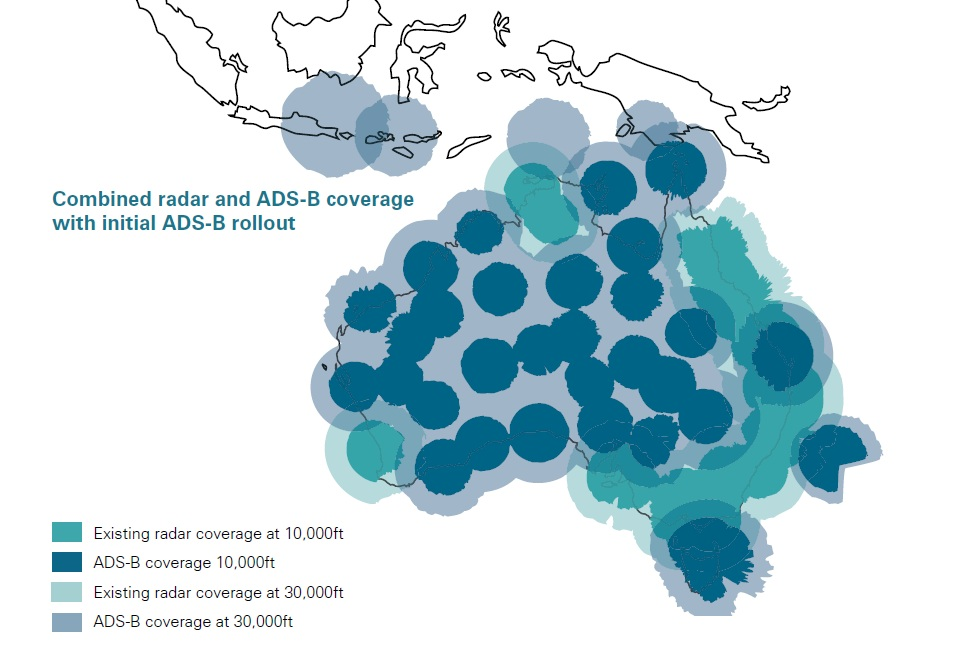
\includegraphics[scale = 0.5]{Pictures/adsb_coverage.jpg}
	
	\caption[ADS-B and radar coverage in Australia]{ADS-B and radar coverage in Australia, reproduced from \cite{ADSB_CASA_booklet}}
	\label{fig:adsb_aus_coverage}
\end{figure}

Out of the range of these ground stations, aircraft tracking via ADS-B is not possible.  Although comprehensive coverage is currently being implemented in Australia \cite{ADSB_CASA_booklet}, the Asia-Pacific region \cite{ADSB_ICAO_man} and much of North America \cite{ADSB_DOT}, there still exists areas, particularly over oceanic and polar regions where the service is not available. Figure \ref{fig:adsb_us_coverage} shows the state of ADS-B coverage in US as of 30/06/2013.
\begin{figure}[H]
	\centering
	\includegraphics[scale = 0.5]{Pictures/adsb_coverage_US.jpg}
	
	\caption[ADS-B coverage in the US as of 30/06/2013]{ADS-B coverage in the US as of 30/06/2013, reproduced from \cite{NextGEN_coverage_map}}
	\label{fig:adsb_us_coverage}
\end{figure}
Some solutions exist for ADS-B coverage in remote and marine areas. Areas where ADS-B is not adequately covered is illustrated in Figure \ref{fig:adsb_nocoverage}, as  estimated by \cite{ADS-B:Aireon_brochure}. Ground stations installed on oil platforms currently provide coverage over the Gulf of Mexico \cite{ADSB_DOT}. Both Globalstar \cite{ADS-B:Globalstar_webinar} and Iridium NEXT \cite{ADS-B:Aireon_brochure} propose global coverage via Low Earth Orbit (LEO) satellite constellations to be launched in 2014.
\begin{figure}[H]
	\centering
	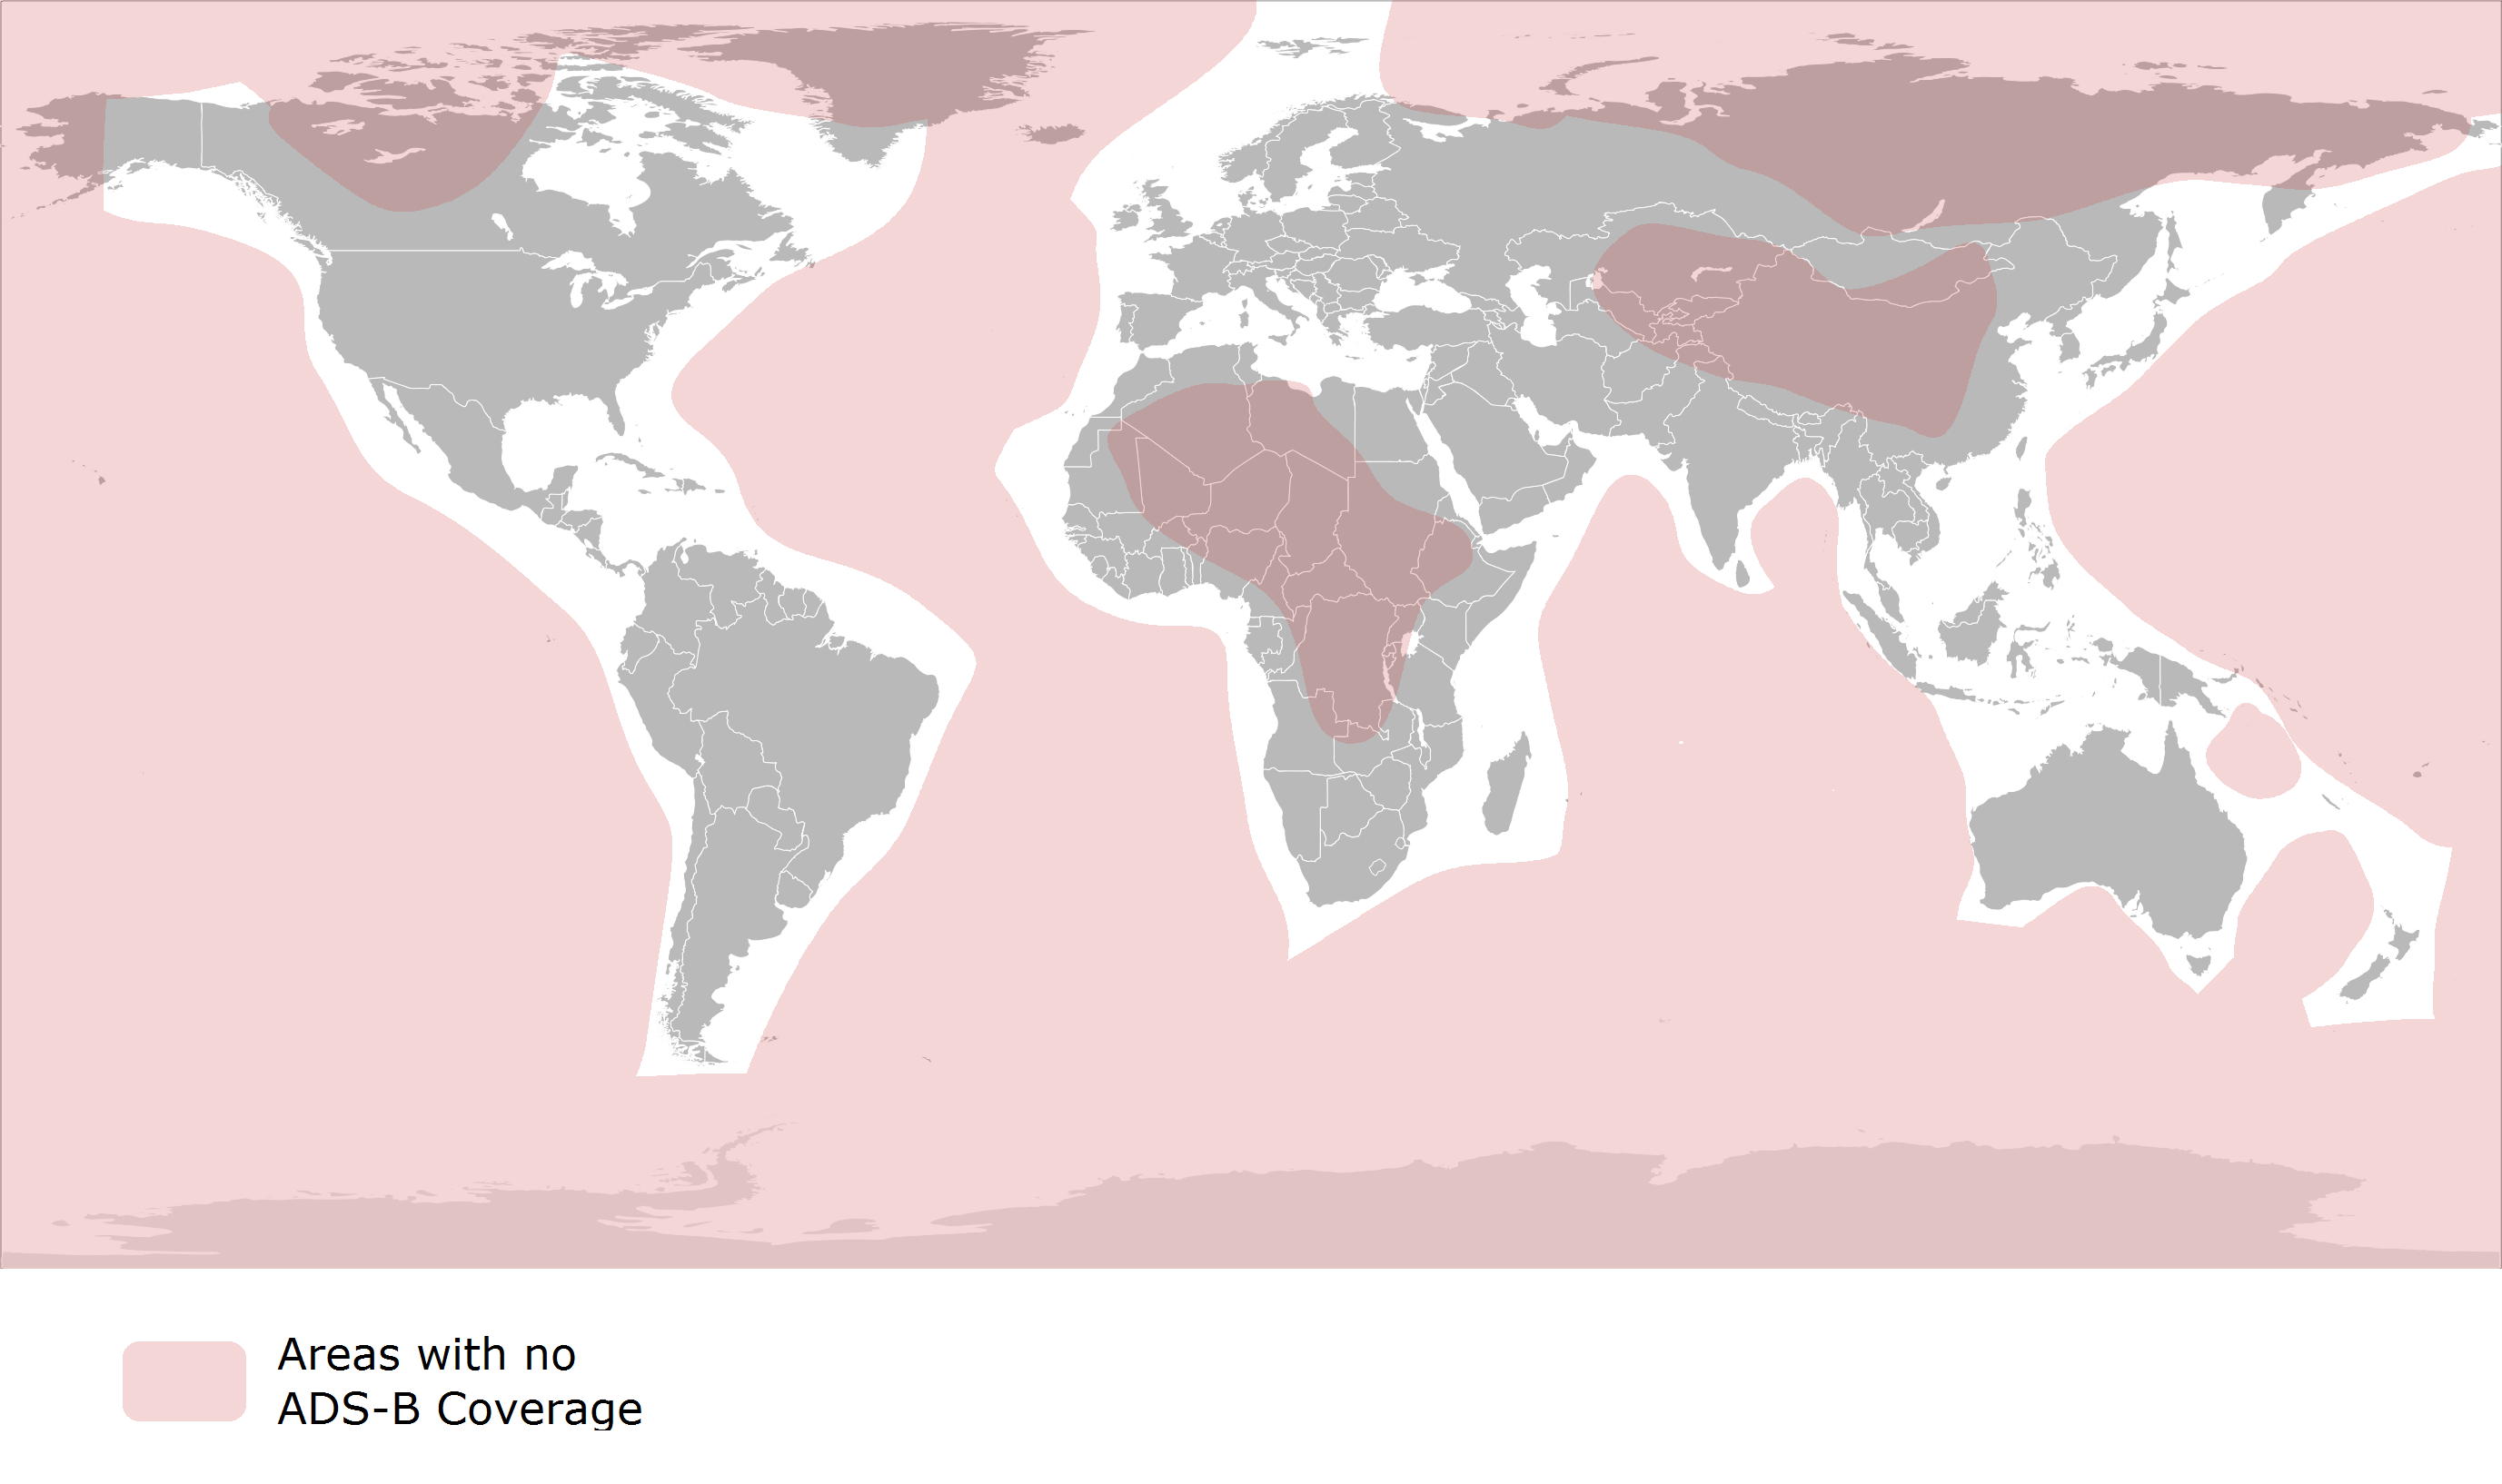
\includegraphics[scale = 0.23]{Pictures/adsb_nocoverage.png}
	
	\caption[Global areas without ADS-B coverage]{Global areas without ADS-B coverage, as estimated by \cite{ADS-B:Aireon_brochure}}
	\label{fig:adsb_nocoverage}
\end{figure}

\newpage
\subsection{Cubesats}
CubeSats are a family of pico-satellites whose mechanical and launch-interface subsystems conform to an open-source standard \cite{Lee2011}. These satellites are characterised by the number of `units' they contain. Each `unit' defines a roughly 100$\times$100$\times$100mm cube-shaped physical envelope and a 1kg maximum weight. Satellites with multiple `units' have a greater mass and payload volume budget. An example of a 2-unit (2U) CubeSat is shown in Figure \ref{fig:2U_example}.

\begin{figure}[H]
	\centering
	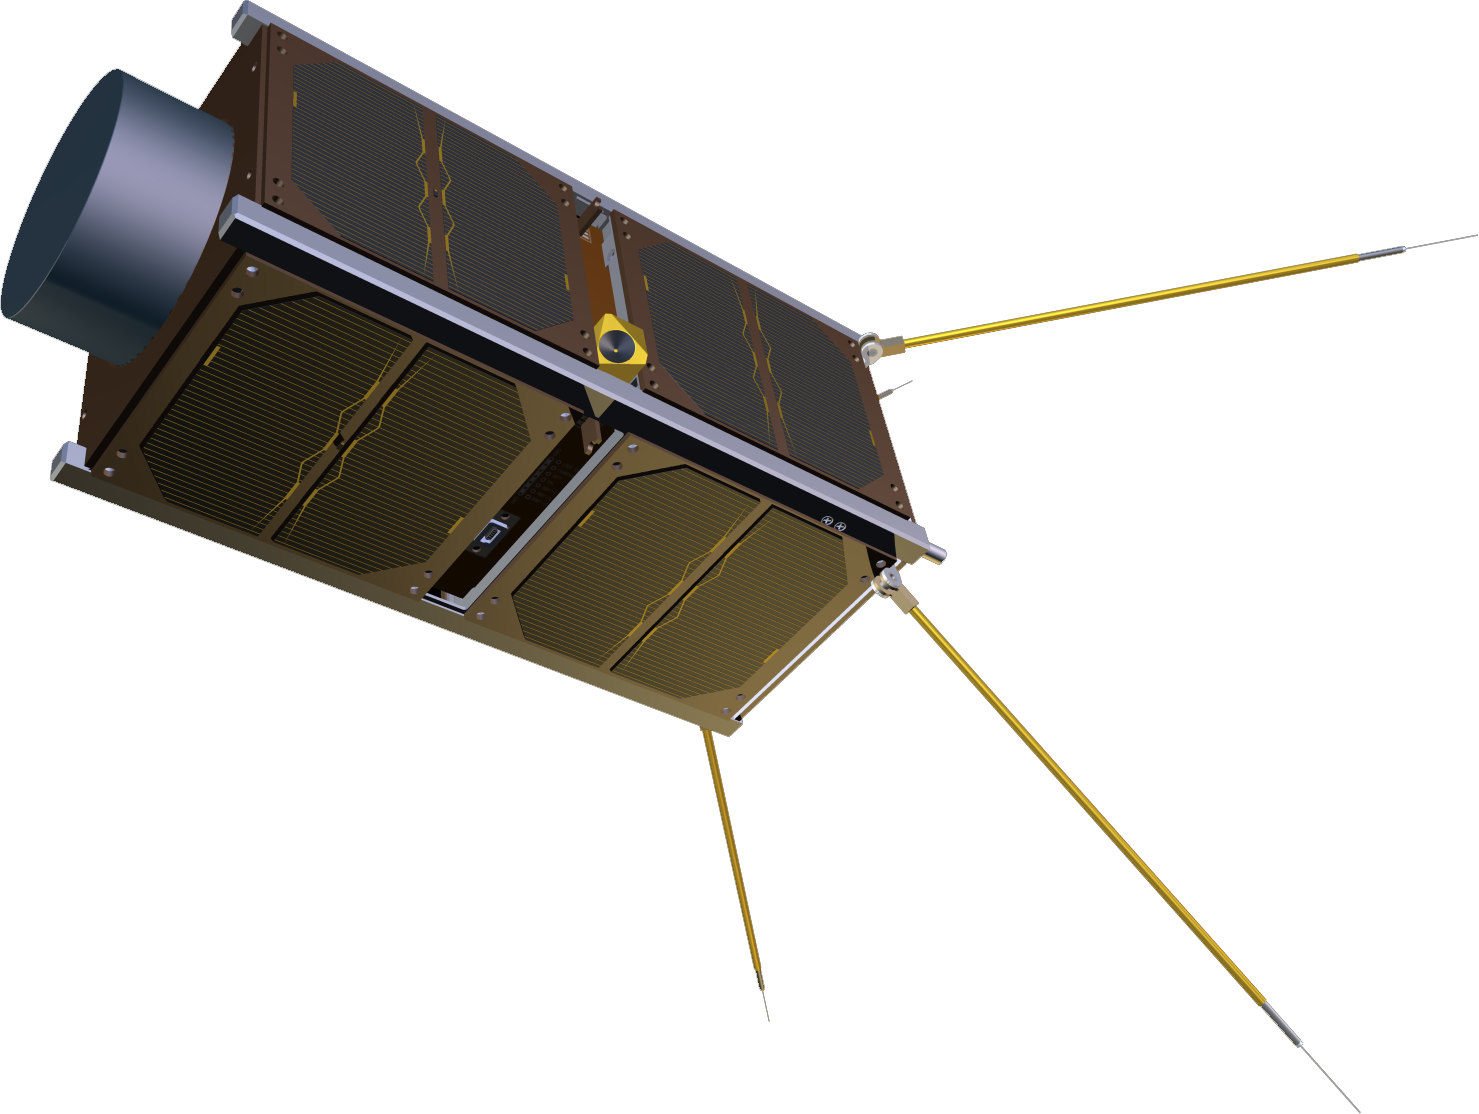
\includegraphics[scale = 0.2]{Pictures/QB50-platform.png}
	
	\caption{The GOMSpace QB50 Platform - an example of a 2U CubeSat, reproduced from \cite{GomSpace2013}}
	\label{fig:2U_example}
\end{figure}

The size and standardisation of CubeSat design have made them accessible to non-military and non-commercial space interest groups, including academic and hobbyist groups. The launch interface design is such that multiple CubeSats can be launched on the same vehicle at reduced cost \cite{Nason2002}. The proliferation of open-source CubeSat designs has allowed the academic and hobbyist community to collaborate and refine CubeSat design concepts. The resulting reduction in design and launch makes developing space-bound payloads more accessible with less risk. Due its reduced size, CubeSats do not have provision for significant orbital manoeuvres and are restricted to LEO missions. 

\subsubsection{Specifications}
Generic CubeSat specifications are given by the California Polytechnic State University (Cal Poly) \cite{Lee2011}. These specifications identify a basic mechanical envelope, materials to be used and a standard launch interface.

Generally, a CubeSat consists of a stacked cube-configuration with 4 rails, each running along the edges of the satellite parallel to the Z axis. Launch and separation switches are located on the bottom face of each of these rails. The design of generic CubeSats is shown in Figure \ref{fig:cubesat_sizes}.

\begin{figure}[htb]
	\centering
	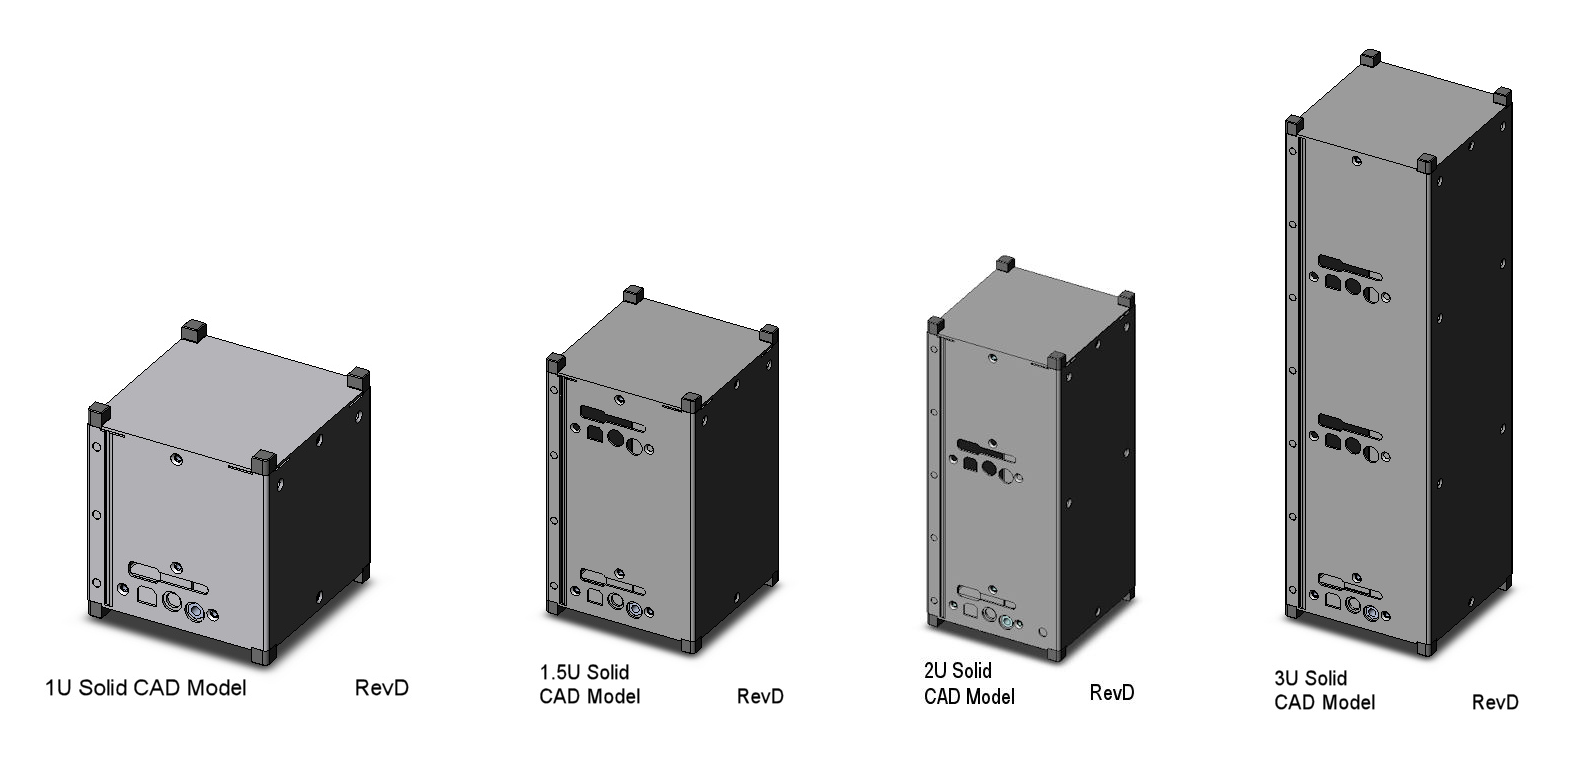
\includegraphics[scale = 0.3]{Pictures/cubesat_sizes.png}
	
	\caption{CubeSat sizes, ranging from the single 1U to the triple 3U. Reproduced from \cite{CubeSatKit2013}}
	\label{fig:cubesat_sizes}
\end{figure}

\subsubsection{Typical Applications}
CubeSats are heavily used by the academic due to their cost-effectiveness and the low-risk associated with mission and platform development. Subsequently the majority of CubeSat missions are associated with academic studies. Satellites such as the University of Toronto's CanX-1 \cite{CanX-1} and the University of Tokyo's XI-V \cite{XI-V} were built to prove the respective university's capability for space technology development.

\newpage
\subsection{Satellite Constellations}
Satellite constellations define a number of satellites in a particular configuration. Constellations are often used when the coverage, downlink opportunities or system update rate provided by a single or two satellites is not sufficient. The GNSS constellations, for example the GPS or GLLONASS constellations, provide global GNSS coverage from a number of satellites in different medium earth orbits (MEO). Satellite communications are provided from LEO constellations, such as the Iridium and Globalstar constellations discussed in more detail below.

In order to define a constellation of circular orbits, the following orbital elements need to be defined for each satellite
\begin{itemize}
	\item \textbf{Altitude}
	\item \textbf{Inclination}
	\item \textbf{Right Angle of Ascending Node (RAAN)}
	\item \textbf{True Anomaly}
\end{itemize}

\subsubsection{Iridium} \label{sec:iridium}
The Iridium Satellite Constellation is a network of 66 LEO satellites which provide mobile communication services over a truly global coverage network. The system provides voice and data coverage for subscribers equipped with Iridium hardware, including mobile handsets and data modems. The intention is that the system will work in remote areas of the Earth where reliable mobile and wireless data over conventional means (i.e. 3G and emerging 4G technologies) is not available. The current and first generation of satellites has been in operation since 1999 and surpassed 500,000 subscribers in September of 2011 \cite{Iridium_subscribers_2011}.

The space segment of the system consists of 66 satellites in Low Earth Orbit at an altitude of approximately 780km. The satellites are evenly distributed amongst six polar co-rotating planes each spaced 31.6 degrees apart in longitude, with the first and sixth planes counter-rotating and spaced 22 degrees apart \cite{iridium_ICAO_man, iridium:an_overview1998}. The planes have a near circular orbit \cite{Pratt1999} Each orbital plane has 11 satellites evenly distributed across the orbit.  This configuration is shown in Figures \ref{fig:iridium_stk} and \ref{fig:iridium_2d_stk}.
\begin{figure}[H]
	\centering
	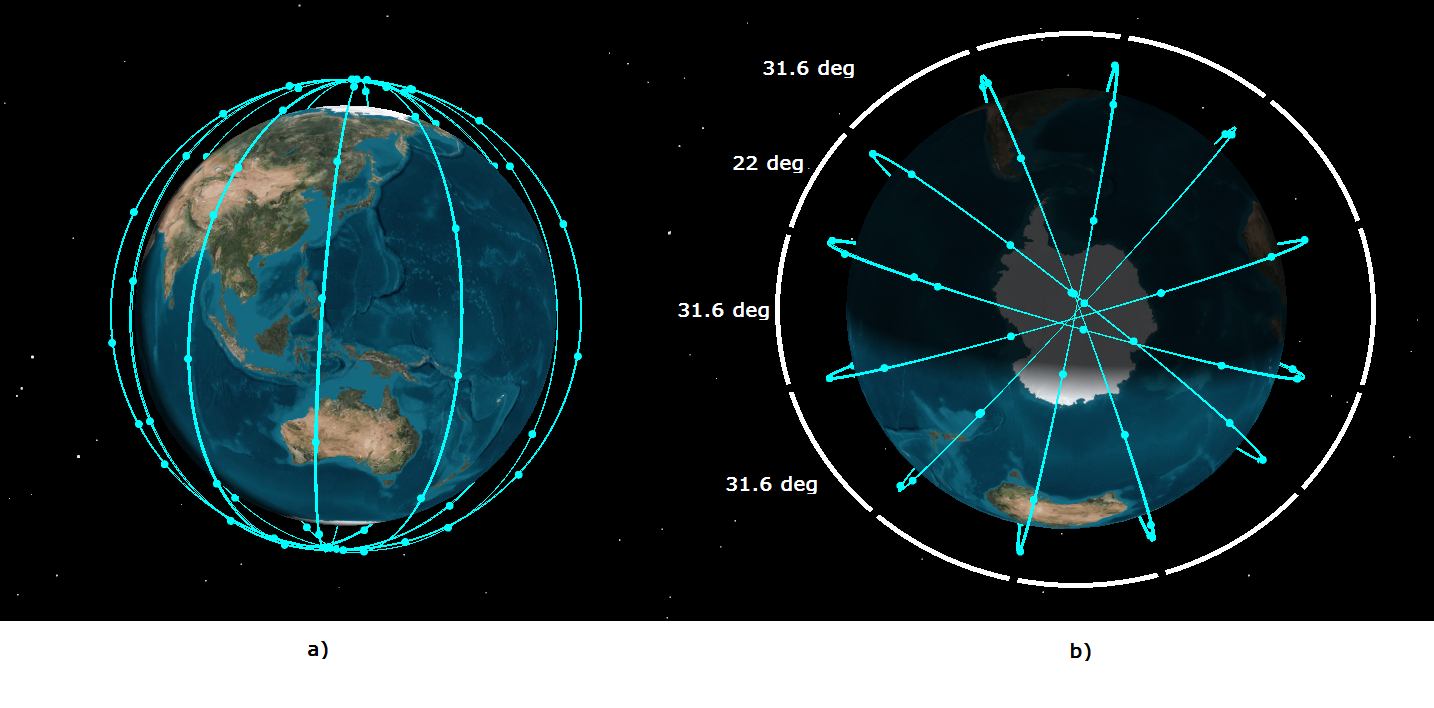
\includegraphics[scale = 0.35]{Pictures/iridium_stk.png}
	
	\caption{Iridium Satellite constellation showing a) a view over Australia and South East Asia and b) the view from above the south pole. Data taken from STK}
	\label{fig:iridium_stk}
\end{figure}
\begin{figure}[H]
	\centering
	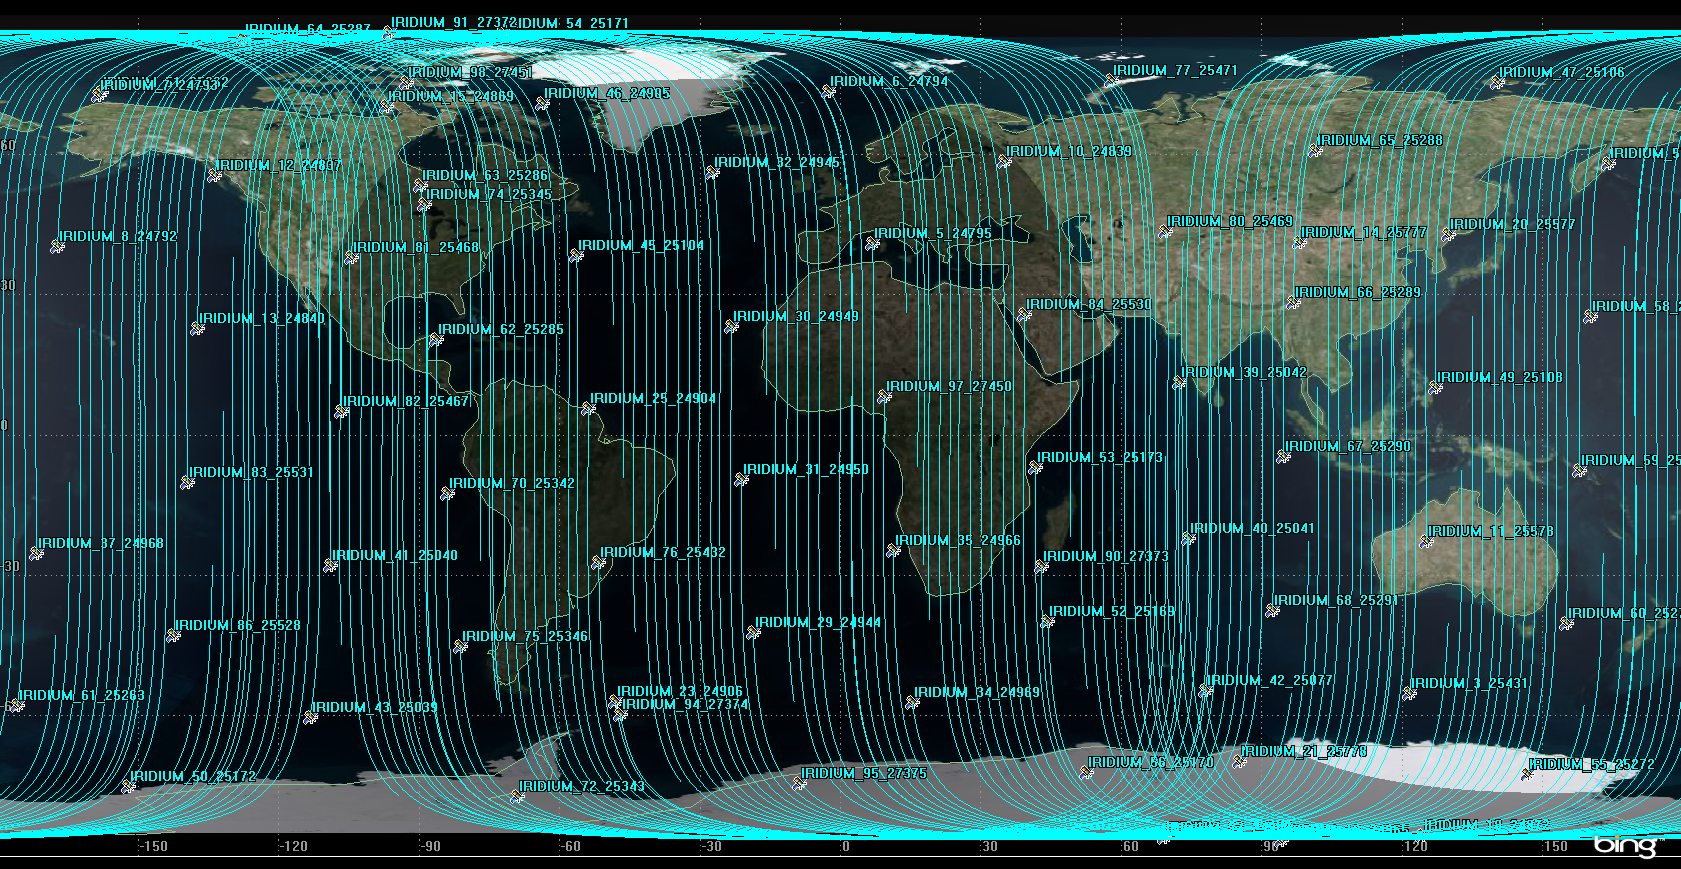
\includegraphics[scale = 0.20]{Pictures/iridium_2d_stk.png}
	
	\caption{Iridium Satellite constellation path over a 2D projection of the surface of the Earth. Data taken from STK}
	\label{fig:iridium_2d_stk}
\end{figure}

\subsubsection{Globalstar}
The Globalstar Constellation consists of 48 LEO satellites that provide mobile communication services that, as far as end-users are concerned, are much the same as those offered by Iridium, as detailed in Chapter \ref{sec:iridium}. Globalstar Inc. provide voice and data coverage over service areas where traditional PSTN data links are not availble. Unlike Iridium, Globalstar does not provide 100 percent global coverage, with swaths only covering areas between $70^\circ$ north and south latitudes \cite{Dietrich1998}.

The space segment of the Globalstar system consists of 48 satellites equally distributed in eight orbital planes. Each orbital plane contains 6 satellites has a $52^\circ$ inclination\cite{Smith1996, Dietrich1998}. Data from STK indicates that the orbits have equally spaced right ascensions of ascending node (RAANs) between $0^\circ$ and $360^ \circ$, offset $45^\circ$ from each other. Each satellite is in a roughly circular orbit, with an altitude of 1414 kilometres \cite{Smith1996} and a period of approximately 115 minutes. The eight orbital planes are illustrated in Figure \ref{fig:globalstar_stk}, with the ground track of all 48 satellites shown in Figure \ref{fig:globalstar_2d_stk}.
\begin{figure}[H]
	\centering
	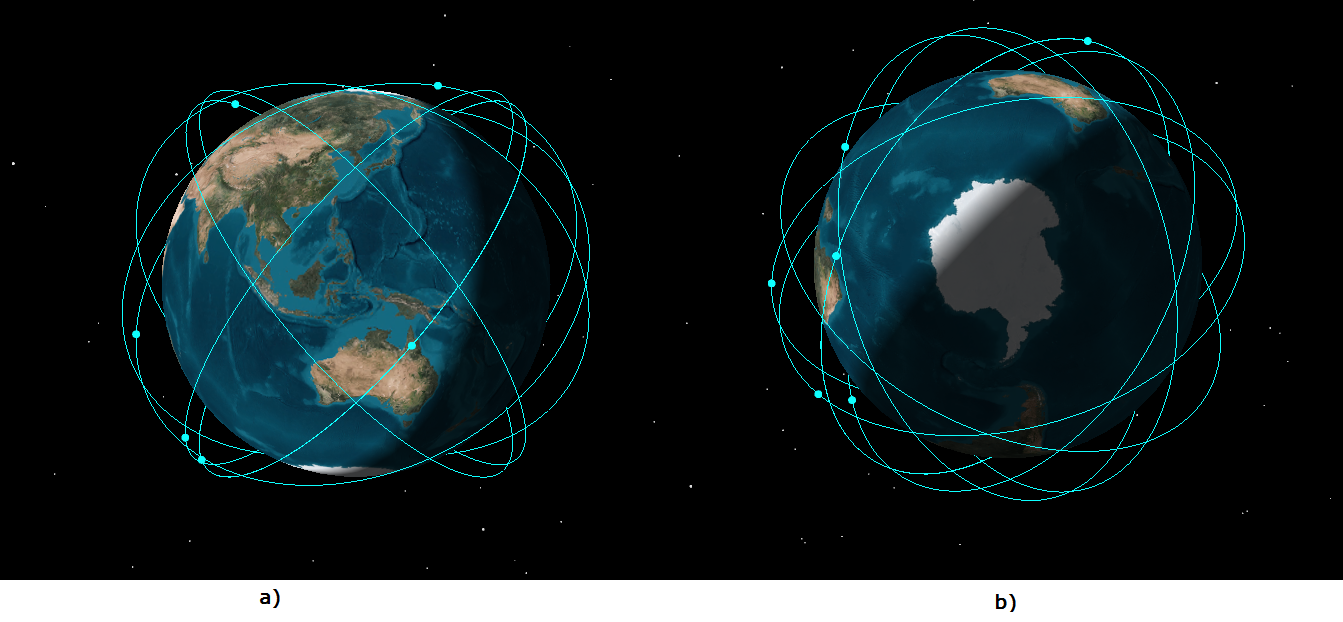
\includegraphics[scale = 0.40]{Pictures/globalstar_stk.png}
	
	\caption{The 8 Globalstar Orbital planes as shown from a) above Australia and South East Asia and b) above the south pole. Data from STK}
	\label{fig:globalstar_stk}
\end{figure}

\begin{figure}[H]
	\centering
	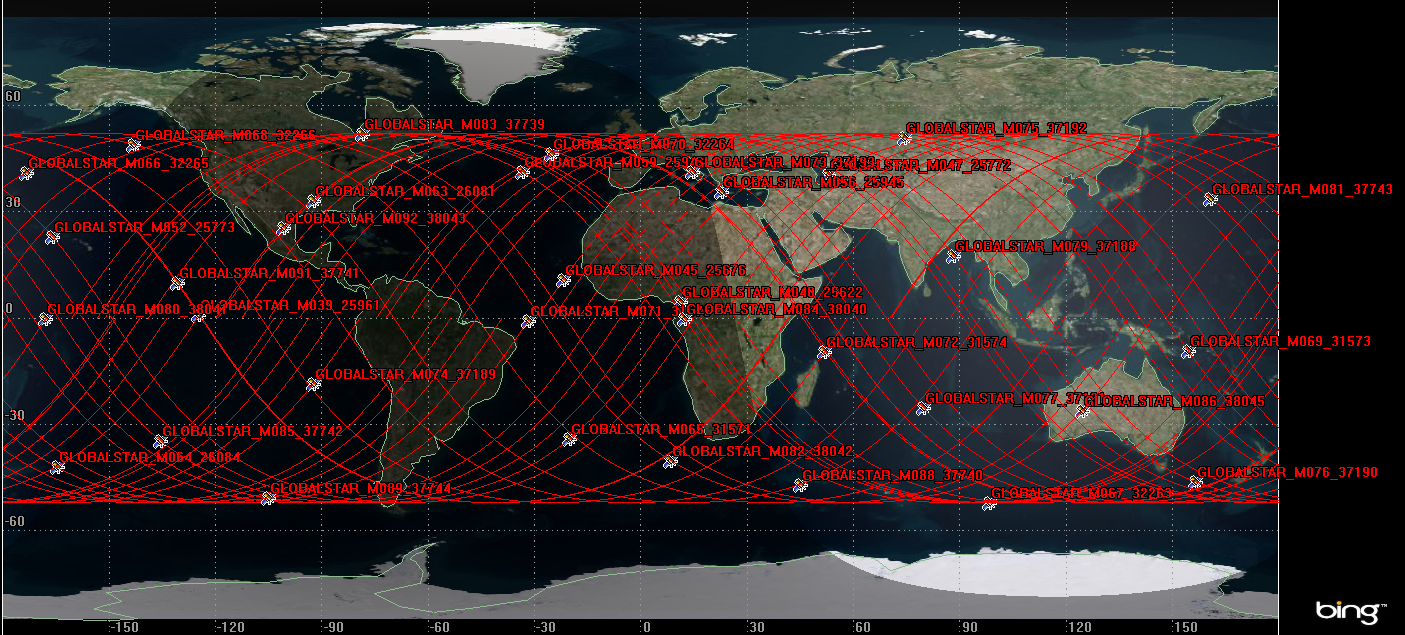
\includegraphics[scale = 0.40]{Pictures/globalstar_2d_stk.png}
	
	\caption{The Ground Track of the 48 Globalstar Satellites. Data from STK}
	\label{fig:globalstar_2d_stk}
\end{figure}


\section{Literature Review}\label{sec:litreview}
A number of academic and commercial groups have shown interest in the concept of developing a space-based ADS-B receiver network. Globalstar and Iridium have committed to delivering constellations with full global coverage, piggybacking on their satellite phone network. Thales, ESA and GomSpace have each developed their own small-satellite ADS-B receivers.

\subsection{ADS-B Link Augmentation System (ALAS)}
ADS-B Technologies have developed the ALAS as a space-based ADS-B coverage solution. The ALAS will be flown as hosted payloads on the Globalstar's second generation constellation of satellites. The system is expected to provide global coverage with a one-second update rate \cite{ADS-B:Globalstar_webinar}.

The ALAS is intended to operate by relaying ADS-B data (received via the normal L and S band transmissions) to ground based gateways through the C band. These gateways would then relate that data to Air Traffic Management (ATM) systems as necessary. The system would be full duplex and is designed to transparently augment the existing ADS-B ground coverage network. This operation is illustrated in Figure \ref{fig:alas_overview}
\begin{figure}[htbp]
	\centering
	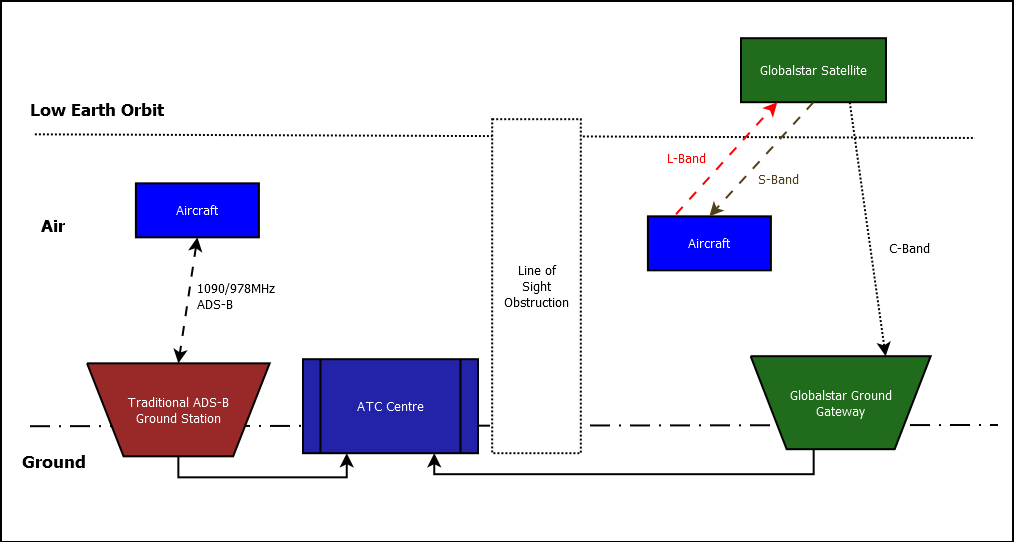
\includegraphics[scale = 0.40]{Pictures/alas_overview_tn.png}
	
	\caption[Overview of the ALAS system]{Overview of the ALAS system, after \cite{ADS-B:Globalstar_webinar}}
	\label{fig:alas_overview}
\end{figure}
This is intended to be an indirect link that requires on-board aircraft to install additional C-band transponders. In this sense it would not be a true `drop in' service. Complete ADS-B coverage using this system would incur significant cost to pilots and aircraft manufacturers.

ADS-B Technologies reported that the second generation Globalstar constellation will provide coverage over most continental areas, with minimal coverage over international waters \cite{ADS-B:Globalstar_webinar}. This is illustrated in Figure \ref{fig:globalstar_adsb}.
\begin{figure}[H]
	\centering
	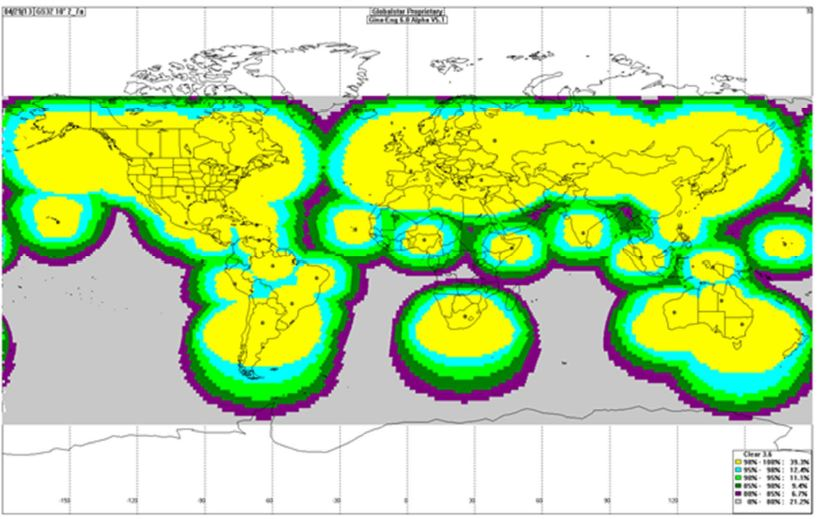
\includegraphics[scale = 0.7]{Pictures/globalstar_asdb.jpg}
	
	\caption[ADS-B Duplex coverage provided by the second generation Globalstar constellation]{ADS-B Duplex coverage provided by the second generation Globalstar constellation, reproduced from \cite{ADS-B:Globalstar_webinar}}
	\label{fig:globalstar_adsb}
\end{figure} 

ALAS would have two major shortcomings -
\begin{enumerate}
	\item The system would require both ANSPs and Aircraft to purchase additional L and S band transceivers to communicate with the space segment. ALAS would not be compatible with standard ADS-B hardware implementation. 
	\item The second Globalstar constellation would have limited coverage due to its orbit configuration and communication infrastructure. The inclination of the Globalstar orbits would not provide ADS-B coverage over the poles, and would rely on a permanent link with ground stations restricts the predicted coverage to continental areas. This is illustrated in Figure \ref{fig:globalstar_adsb}.
\end{enumerate}

ALAS is expected to be operational in late 2014 \cite{ADS-B:Globalstar_webinar}. ADS-B Technologies have not yet released any information about buy-in models for ANSPs.

\subsection{Aireon} \label{sec:aireon}
As of June 2014, Aireon LLC were developing an space-based, ADS-B reliant `global aviation surveillance system' \cite{ADS-B:Aireon_brochure} to be flown on the Iridium NEXT constellation of LEO satellites. The constellation was expected to provide complete global coverage, including over polar regions \cite{ADS-B:Aireon_comparison}.   

This system was presented as flight path solutions for both ANSPs and commercial airlines. Marketing material claimed that intelligent flight path planning will save airlines fuel costs with more optimised routes \cite{ADS-B:Aireon_comparison}. No independent analyses or verifications of these claims were found. The service was expected to be available by 2017.

The concept presented for the system suggested that unlike the Globalstar hosted ALAS, Aireon would use the standard Mode S Extended Squitter carrier signal in order to receive ADS-B signals\cite{Dawson2013}. This concept is illustrated in Figure \ref{fig:aireon_concept}. This had a distinct advantage in that no additional hardware is required in order to implement the system. 

\begin{figure}[htbp]
	\centering
	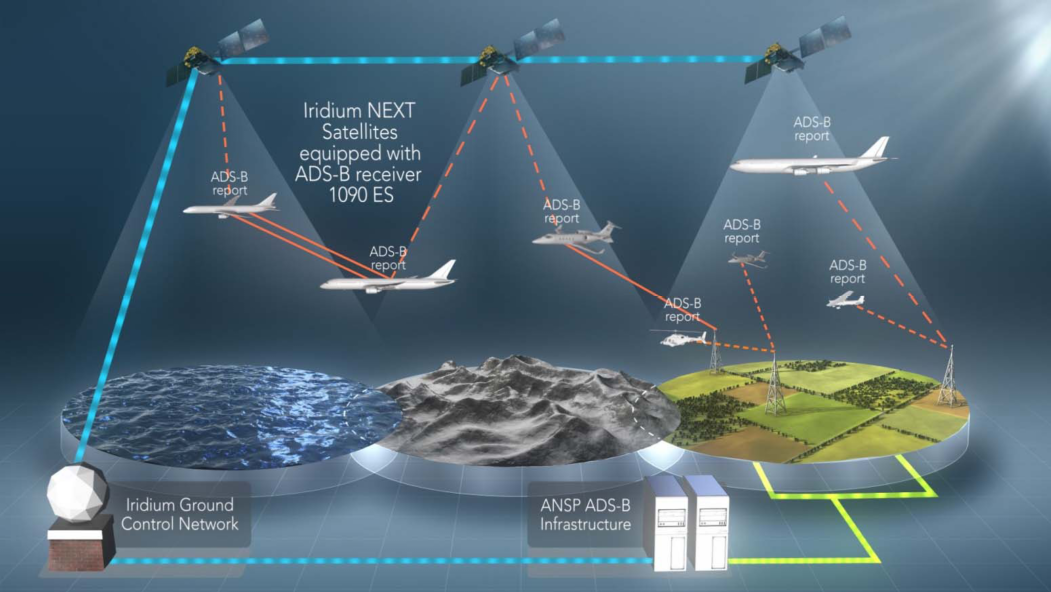
\includegraphics[scale = 0.55]{Pictures/aireon_concept.png}
	
	\caption[Aireon System Concept]{Aireon System Concept, reproduced from \cite{Dawson2013}}
	\label{fig:aireon_concept}
	\end{figure}

Details on the intended orbit and performance standards for the Iridium NEXT constellation had not yet been made publicly available. Descriptions of the Iridium NEXT's intended services suggested that the orbital configuration and control model would be similar to the first Iridium constellation discussed in Section \ref{sec:iridium}  \cite{ADS-B:Aireon_brochure}. 

Although this provided the complete coverage required by the problem statement, it was expected that the cost-model for the system will be quite high. The launch and operations of the first Iridium constellation was complex and costly enough such that mismanagement of the project's investment and return resulted in Iridium filing for bankruptcy a year after the launch of the final satellite in August 1999 \cite{Finkelstein2000}.   The total project and operations cost of a smaller CubeSat constellation would be much lower and therefore have significantly less risk. The solution put forward in this thesis could prove to be more economically effective.

\subsection{Spaced Based ADS-B In-Orbit Demonstration Payload (SABIP)} \label{sec:sadip}
SABIP was presented as space-based ADS-B receiver system designed to operate over the standard Mode S 1090MHz carrier signal currently being developed by Thales Alenia Space Deutschland. The successful implementation of this receiver would enable ADS-B signals to be relayed from LEO without extra infrastructural cost. Specifically, existing Mode S transponders used by aircraft and ANSPs could still be used without significant augmentation to existing equipment. The system was intended to receive and record ADS-B messages, decode those messages and then assemble reports that can be transmitted to ground stations and ANSPs \cite{Blomenhofer2012}. 

The research put forward that the chief challenge in designing the receiver was mitigating signal degradation due to high-density traffic. The Mode S frequency is time-shared for both ADS-B transmissions and Traffic Collision Avoidance Systems (TCAS) for all aircraft. The enlarged antenna footprint from LEO meant that both of these signals need to be detected and processed for a high number of aircraft. The footprint of a receiver from LEO would have a radius of approximately 3200 nautical miles whilst a terrestrial Mode S receivers typically have a footprint of 200 nautical miles. This degraded the detection of squitter signals over Mode S transmission \cite{Blomenhofer2012}. 

The proposed solution consisted of an ADS-B antenna which has multiple spot beams, each covering a limited area. The models of this antenna are shown in Figure \ref{fig:sapid_spotbeams}. The exact number and configuration of spot beams had yet to be determined and required further study of signal degradation due to transmission density \cite{Blomenhofer2012}.

\begin{figure}[htb]
	\centering
	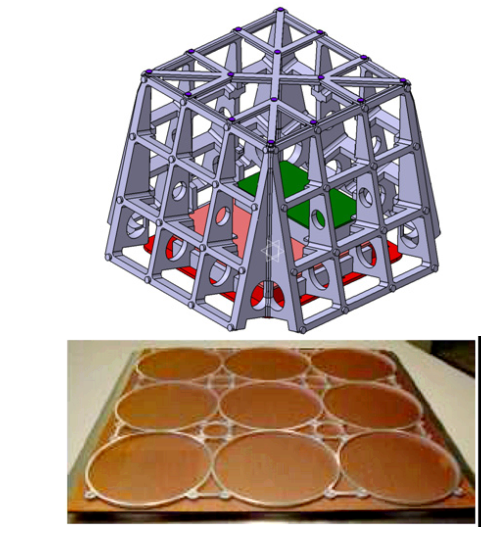
\includegraphics[scale = 0.8]{Pictures/sapid_spotbeams.png}
	
	\caption[SAPID receiver Antenna design]{SABIP receiver Antenna design, reproduced from \cite{Blomenhofer2012}}
	\label{fig:sapid_spotbeams}
\end{figure}

This research identified the key need to deal with signal collisions and maintaining a high probability of aircraft detection. In particular, the issues with detection probability given a high number of aircraft agree with the Mode S receiver requirements described in \cite{Orlando2001}. This means that re-visit time and scan time for a particular area on Earth will be key parameters in evaluating the effectiveness of any given ADS-B constellation

The technology developed by Thales could also form a foundation for the implementation of a CubeSat based ADS-B receiver system. Signal collision and resolution problems outlined in the paper would be experienced by any in-orbit ADS-B receiver. Although the exact antenna dimensions prohibit SABIP from being incorporated into a CubeSat form-factor, the same design principles would need to be incorporated into a the design of a more suitably sized receiver. Similarly the data storage and analysis framework put forward in \cite{Blomenhofer2012} could be used for the ground and space segment of the ADS-B system. The research indicated that the technology required for a spaced based ADS-B receiver is certainly possible in the CubeSat form factor.


\subsection{Proba V}
In early 2013, the European Space Agency (ESA) launched their fifth experimental Proba satellite, Proba V, with a guest ADS-B Payload. Like SABIP, the ADS-B payload is designed to receive signals via the native Mode S 1090Mhz carrier. The receiver, designed by the German Aerospace Center (DLR) was designed to receive ADS-B from LEO in Proba V's 820km orbit \cite{DLR,TheEur,T}. Proba V is travelling in a Sun-Synchronus polar orbit at an altitude of 820km \cite{TheEur}.  

As of June 2014, the satellite was tracking Aircraft over Northern Europe \cite{DLR}. Tests to determine the sensitivity of the receiver to issues caused by signal density (as put forward by \cite{Blomenhofer2012}) were ongoing. Figure \ref{fig:probav_planes} shows the results from the initial proof of concept, with aircraft being detected in Europe\cite{TheEur}. No further results beyond this proof of concept have been published. However this provided further evidence for the viability of receiving ADS-B signals from LEO, particularly from an altitude as high as 820km.
\begin{figure}[H]
	\centering
	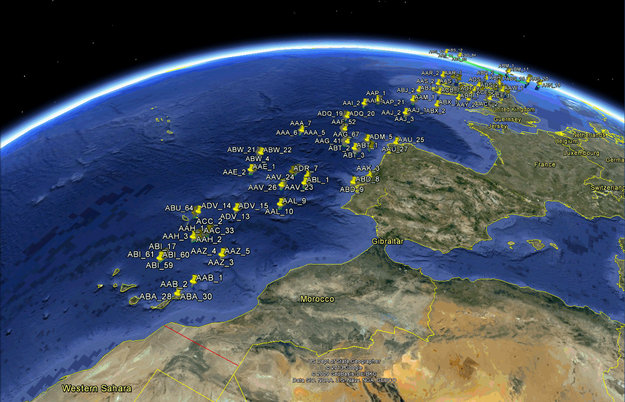
\includegraphics[scale = 0.5]{Pictures/probav_planes.jpg}
	
	\caption[Aircraft detected by Proba V over Europe]{Aircraft detected by Proba V over Europe, reproduced from \cite{TheEur}}
	\label{fig:probav_planes}
\end{figure}

\subsection{GOM-X1} \label{sec:gomx}
The GOM-X1 was a 2U CubeSat intended to perform a number of space based experiments using software defined radio (SDR), the primary being a a spaced based ADS-B receiver. The satellite was developed as a collaborative effort between GomSpace, DSE Airport Solutions (now Insero Software \cite{Insero2014}) and Aalborg University. The primary mission of the satellite was to demonstrate that ADS-B reception is capable from a CubeSat platform in LEO. Data received from onboard sensors would be compared with ground-based ADS-B data to verify the correctness of the data acquired from LEO\cite{GomSpace2014,Alminde2012}.

ADS-B signals were to be received via a custom SDR payload. The SDR is designed to be able to have a reconfigurable decoder structure. The intention of the experiments was to evaluate the effectiveness of different decoder configurations. This data would be used for further refinements to space based ADS-B CubeSat modules. A helical receiver antenna is used in order to maximise the gain going into the system, pictured in Figure \ref{fig:gomx_antenna}.  GOM-X1 used a standard commercially off-the-shelf (COTS) bus available from GomSpace\cite{Alminde2012}.
\begin{figure}[H]
	\centering
	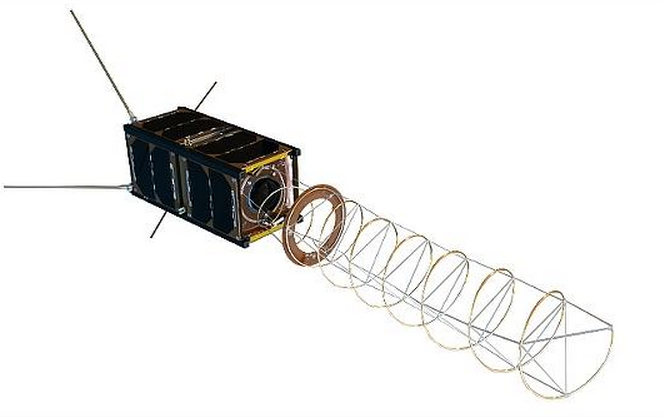
\includegraphics[scale = 0.5]{Pictures/gomx_antenna.png}
	
	\caption[3D render of the GOM-X1 satellite, showing the expanded helical receiver antenna]{3D render of the GOM-X1 satellite, showing the expanded helical receiver antenna, reproduced from \cite{GomSpace2014}}
	\label{fig:gomx_antenna}
\end{figure}
The satellite was successfully launched in November of 2013 into an circular orbit of 600km altitude and 97.8 degrees of inclination. GOM-X was still `fully commissioned' and operational in June of 2014\cite{EoPortal, GomSpace2014}. GomSpace released a `preliminary plot' of the received aircraft positions, reproduced in Figure \ref{fig:gomx_planes}, showing detected aircraft mostly in the northern hemisphere. 

\begin{figure}[htbp]
	\centering
	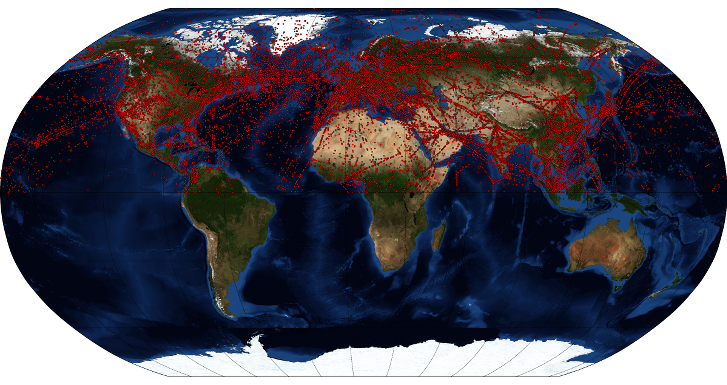
\includegraphics[scale = 0.8]{Pictures/gomx_planes.png}
	
	\caption[Preliminary plot of planes detected by GOM-X1]{Preliminary plot of planes detected by GOM-X1, reproduced from \cite{GomSpace2014}}
	\label{fig:gomx_planes}
\end{figure}

The early success of the mission provides a good indication of the viability of a CubeSat based ADS-B receiver. However no data is provided on the quantitative performance of the receiver. Of particular interest would be the aircraft detection rate of a given pass or scan of the satellite. Being able to determine the statistical likelihood of aircraft detection from the GOM-X1 would provide a hard systems constraint for the design of a CubeSat constellation. The data presented in this thesis will instead provide a range of constraints on the sensitivity of the required ADS-B receiver from the analysis of proposed constellations  


\begin{comment}
\subsection{Automatic Identification System (AIS)}
The Automatic Identification System (AIS) is the maritime analogue to ADS-B. The system consists of VHF transponders which relay ship telemetry (identity, heading, destination etc.) between ships and between ships and shore stations. The viability of augmenting AIS with a LEO space-segment has been in investigation since 2003 \cite{Hoye2008}. The primary goal of the proposed Satellite AIS systems is to provide route monitoring, allowing for longer update periods and data-lag. 

\subsubsection{Satellite-based Receivers}
The key challenge with Satellite-based AIS, as with ADS-B, is the detection of signals in high density areas where signal collision is prominent. Low density areas with less than 2000 ships will yield a detection rate of 99\% from conventional AIS receivers \cite{Hoye2008, Carson-Jackson2012}. This number drops off significantly as more ships enter the antenna footprint, dropping as low as 50\% with 2500 ships for an observation time of 15 minutes \cite{Hoye2008}. There are two design solutions to mitigate this issue \cite{Hoye2008, Carson-Jackson2012, Scorzolini2010}:
\begin{itemize}
	\item Increase observation time by decreasing the period between satellite revisits and allowing multiple passes to happen over a given area. This introduces extra infrastructural costs, requiring more satellites and ground stations to maintain 
	\item Designing AIS receivers to have narrow-footprint spot beams, decreasing the number of ships and chance of signal collision for a particular receiver. This decreases the area of effectiveness for one satellite and may necessitate more satellites to support the entire system.
\end{itemize}
Both exactEarth \cite{Exact} and ORBCOMM \cite{ORBCOMM} produce AIS receivers designed for flight on LEO micro-satellites. ORBCOMM have launched two LEO satellites containing their AIS receiver, one in an equatorial orbit and the other in a polar orbit. The company claims that these two satellites provide "complete global AIS coverage" but do not specify at what update rate. ORBCOMM will launch an additional 17 AIS equipped LEO satellites in 2013 at unspecified orbital configurations \cite{ORBCOMM}. The current ORBCOMM constellation is inclined at various inclinations and altitudes, determined by system requirements at time of individual satellite deployment \cite{Tandler1996}.

\subsubsection{Proposed Constellations}
The constellation designs put forward for Satellite AIS are less ambitious than Space Based ADS-B solutions, providing longer update rates. \cite{Hoye2008} claims that four constellations in 4 identical and equally spaced orbital planes at an inclination of $58^\circ$ will provide  global coverage with an update rate of once per hour. This figure can be doubled with 8 satellites \cite{Hoye2008}.

A study released by the Telespazio puts forward three scenarios, each dependant on the nature of the ground-station network\cite{Scorzolini2010}:
\begin{enumerate}
	\item Six satellites in six sun synchronous orbits delivering an update rate of less than 3 hours. The revisit time for each point on Earth would be less than 2 hours. The data would have an update lag of 1 hour.
	\item Twelve satellites in 6 orbital planes with an update rate of less than one hour. This number would increase to 25 if multiple passes are needed to ensure detection integrity. The update lag is claimed to be lower than 30 minutes.
	\item Ten satellites in an unspecified orbit with an update time of 1.5 hours and update lag of 45 minutes.
\end{enumerate}
The exact orbital configuration and ground station network was not specified.

An ESA sutdy specifies an AIS system with a 3 hour reporting interval that uses  6-8 Satellites at an altitude of approximately 600km "with proper orbit design" \cite{Cervera2008}. This study is expanded upon in \cite{Cervera2011}, where 5 LEO satellites are suggested to be in 5 different orbital planes each with $30^\circ$ difference in RAAN. Inclinations of between $80^\circ$ and $100^\circ$ were suggested, each having different coverage and revisit time trade-offs. Up to 10 satellites in the same configuration may be necessary for high population ship cases \cite{Cervera2011}. 

The performance parameters for each of the Satellite AIS systems investigated do not meet the immediacy requirements of ADS-B. The proposed AIS constellation designs can be mimicked in order to provide basic route monitoring for aircraft, but not live tracking data. However, the technologies investigated and basic system design provide a good base model from which a more immediate system can be designed. In particular, having more satellites and implementing inter-satellite links as per Iridium can drastically improve the update time performance of the proposed system. 

\end{comment}

\subsection{Conclusions}
The survey of current technologies show that there is commercial motivation for the development of ADS-B systems from Space.  ALAS and Aireon represent significant commercial investment in the development of space based ADS-B systems. Although the large commercial risk is absorbed significantly by having the payloads `piggy-back' on the Globalstar and Iridium NEXT constellations, the costs of the buy-in model are not yet known. 

Proba V, SABIP and GOM-X1 demonstrate that there is significant interest in implementing space-based ADS-B on small satellites. Proba V and SABIP are both designed for use on smaller  satellites with the intention of potentially lowering the cost of a space based ADS-B system. Proba V in particular has already demonstrated success, though the quantification of that success is not yet known. The success of GOM-X1 proves that the technology is viable on a CubeSat scale.

These examples show that there is ongoing interest and motivation in developing an economic solution for a space based ADS-B system. The Iridium NEXT and Globalstar constellations provide guaranteed system update and coverage but the design is not necessarily optimised for ADS-B coverage. Given the success of technology demonstrators for small satellites, there is sufficient motivation for development of a low cost ADS-B constellation using CubeSats. 

\newpage
\chapter{Experimental Method and Design}
\label{part:exp_method}
In general terms we were interested in the ability for a given constellation of LEO satellites to provide ADS-B coverage in the absence of land-based ADS-B receivers. To evaluate this, popular flights over the Atlantic and Pacific Oceans were simulated in STK. The simulation was extended to include communication links to LEO satellites. Different satellite constellations were simulated and the link-budget data for each test case was collected. The efficacy of a constellation was determined by comparing the aggregated access times and link budgets for the ADS-B links between a given trans-oceanic flight and the overhead satellites.
\section{Mission Overview}
The root requirement of a satellite-based ADS-B system was the provision of ADS-B coverage over regions where terrestrial systems did not currently provide coverage (in particular, oceans and poles). Within this requirement were a number of variable mission parameters that effected the design and economic cost of resulting satellite systems. Varying the parameters and analysing the performance of resulting designs was used for a mission trade-off analysis, presented in Section \ref{sec:decision_matrix}.

\subsection{System Users}
A spaced based ADS-B system would have two key user groups
\begin{itemize}
	\item Air Navigation Service Providers
	\item Airlines and air transportation service providers
\end{itemize}
Although Australia, America and Europe were able to implement terrestrial ADS-B stations, rolling out terrestrial stations to cover all interest areas was not necessarily cost effective. This was particularly true in regions such as South East Asia. In such areas, the technology and economic base did not exist to make terrestrial deployment viable \cite{Blomenhofer2012}. In these situations a satellite-based system could more effectively augment existing ADS-B coverage for use by ANSPs.

Another key user would be airlines and other air transportation services. Greater position and telemetry coverage of aircraft over oceanic and polar regions would facilitate more optimal flight path co-ordination. ADS-B assisted flight routing would allow for narrower longitudinal and latitudinal track separation, allowing for more flights to travel on desired fuel-saving paths. A flight simulation analysis presented by Iridium LLC suggests that increased density of planes in jet streams can result in fuel savings of up to 450 litres per oceanic flight \cite{Dawson2013}. 


\subsection{System Update Rate}
The update rate of a space-based ADS-B system defined timeliness with which aircraft data can be updated and disseminated terrestrially. Having a high-effective update rate was crucial in range of Airports with ATC towers having to co-ordinate a large density of aircraft traffic. With ADS-B, terrestrial ATC towers typically achieved an update rate of less than 1 second depending on airport capacity \cite{Orlando2001}. For the purposes of live tracking and safety control, an update rate in the order of 1 second to 30 seconds would be required. An update rate in the order of 5 to 10 minutes would enable satisfactory tracking by airlines and air transport services at less cost. A lowest cost system with an update rate of 1-2 hours could be useful for occasional tracking of aircraft making oceanic flights. This, however, would be inadequate for safety applications or any short-range terrestrial flights. 

\subsection{Revisit Time}
Due to the random access nature of Mode S Extended Squitter, the number of aircraft surveyed by an ADS-B receiver was limited. Scanning for a shorter period, or scanning an area with more aircraft would result in more ADS-B collisions and a drastically reduced detect rate. `Missing' aircraft in this manner would be unacceptable from a safety perspective. Suggested solutions for high density areas included more sophisticated antenna design with spot beams \cite{Blomenhofer2012}, or variable-periodicity of ADS-B signals \cite{Orlando2001}. 

For ADS-B reception via satellite, a populated area could be either scanned for a longer period, or `re-scanned' over multiple revisits. This would mediate the need for a larger or more sophisticated and costly antenna array. A longer scanning period could be achieved slowing the ground-track of the space segment over key areas. This would particularly be a problem on CubeSats where technology capability was limited. The revisit time would therefore be defined by limitations of the antennae array and on-board processing technology for ADS-B signal reception. More detail on current small-satellite ADS-B receiver research is discussed in Section \ref{sec:litreview}.
 
\subsection{Geographical Coverage}
Full global coverage would be achieved by a series of polar or near polar orbits, such as the Iridium Satellite constellation \cite{iridium_ICAO_man,iridium:an_overview1998}. Achieving full coverage would be the most costly solution, requiring the largest number of satellites and ground stations. At the very least, the ADS-B system should at least cover the North Atlantic, North Pacific and Indian Oceans and South East Asia in order to meet the root system requirement. These areas had the highest amount of air traffic not covered by terrestrial ADS-B systems as shown in Figure \ref{fig:flightpaths}. Monitoring these regions with specific orbits can reduce the number of spacecraft required in order to provide the coverage gap required by the system. Coverage of the poles would provide extra benefit, opening up polar flight paths.
\begin{figure}[htbpp]
	\centering
	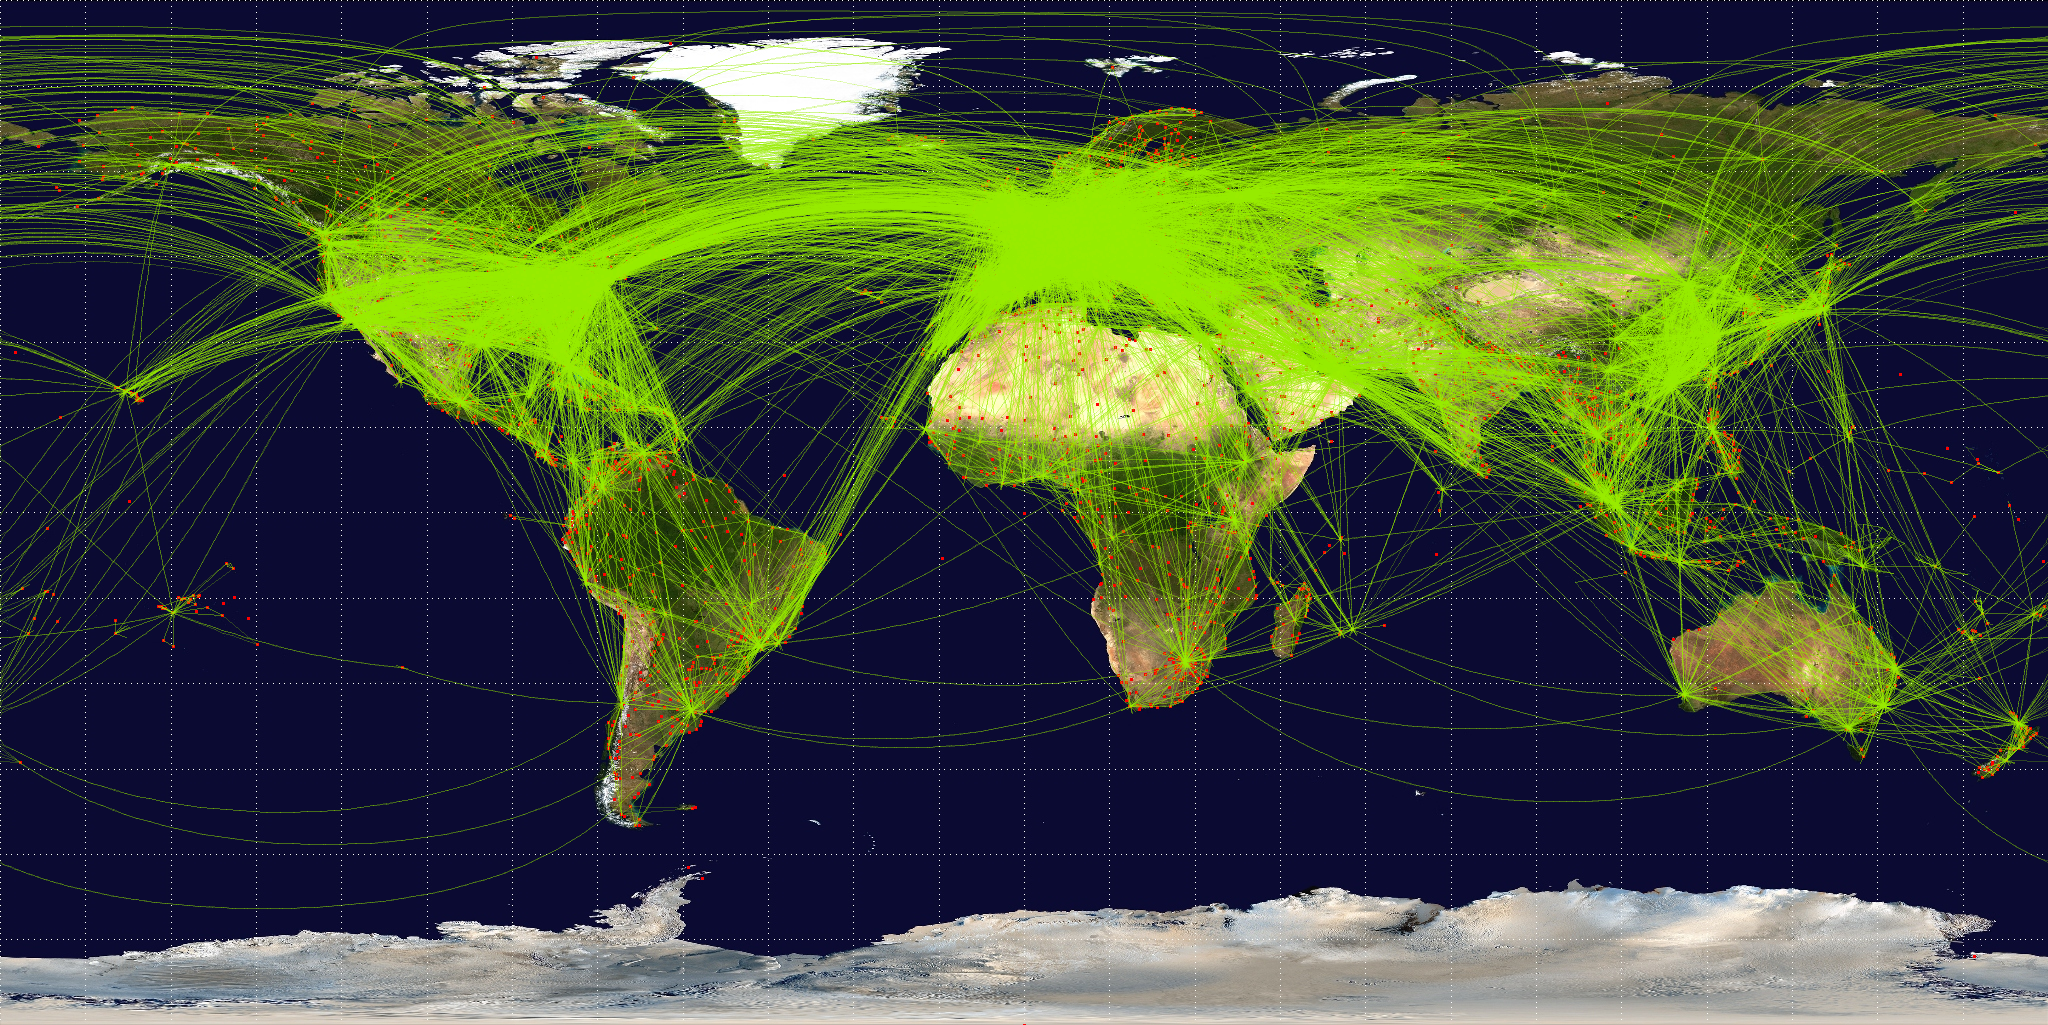
\includegraphics[scale = 0.18]{Pictures/flightpaths.png}
	
	\caption[Popular flight routes]{Popular flight routes, from \cite{Open}}
	\label{fig:flightpaths}
\end{figure} 



\section{Experimental Parameters}
Useful output parameters and input parameters were defined in order to carry out the series of comparative constellation studies. The output parameters from the STK model were used in order to quantify the relationship between constellation input parameters and system performance.
\subsection{Performance Metrics}
\label{sec:perfMetrics}
ADS-B coverage for a each satellite constellation was analysed on a flight-by-flight basis. For a given constellation, the communication link was analysed separately for a sample of trans-oceanic test flights. Each link was characterised by three parameters -
\begin{itemize}
	\item \textbf{Access Times} - the periods of time during which a flight had line-of-sight to at least one overhead satellite and therefore could theoretically establish an ADS-B link. This was available as primary data from STK.
	\item \textbf{Coverage Gap Times} - the periods of time during which a flight has line-of-sight access to no satellites in the constellation. This was calculated after evaluating data from STK.
	\item \textbf{Received Isotropic Power} - the power of the ADS-B signal after it has been propagated from a flight to an overhead satellite. This was available as primary data from STK \footnote{Although the STK communication toolkit was capable of RF link characterisation beyond simply received isotropic power, it was found that the `simple' antenna models used were not adequate for that level of analysis. The results, typified by Table \ref{tab:results_linkbudget_sample1}, show a very high bit-error rate and bad signal-to-noise ratio. The values were such that the development of a signal processing module would be near impossible. A more realistic set of signal characteristics could be achieved by more sophisticated antenna and RF models. However the knowledge required to design the model was beyond the scope of this thesis. Instead, we simply used received power as a comparative indicator of RF performance of the system.}.
\end{itemize}

 
From this data, four values were computed and used as performance metrics to evaluate the efficacy of a constellation - 
\begin{enumerate}
	\item \textbf{Total coverage gap fraction} - the fraction of time a simulated flight spends without being able to transmit ADS-B signals to a satellite. This would be representative of the time the flight would expect to spend out of communication for a given period of time. This was calculated by the formula
	\[ \dfrac{\text{total time with no access to a satellite}}{\text{total analysis time}}\]
	\item \textbf{Maximum gap time} - the maximum amount of time a flight spends without a communication link to a satellite. This represents the worst case scenario for the amount of time a flight would spend out of communication.
	\item \textbf{Average Gap Time} and \textbf{Average Access Time} - the mean of access times and coverage gap times identified during the analysis period. This would give an indication of the periodicity of the 'access-no access' cycles that a flight would experience.
	\item \textbf{Minimum Received Isotropic Power} - the minimum power of an ADS-B signal as it is received by a satellite. This can be used to later determine the link budgets and perform the system definition for a given satellite in the constellation.
	
\end{enumerate}
The relative importance of these performance metrics will be compared in section \ref{sec:decision_matrix}

\subsection{Flight Selection} \label{sec:flight_selection}
OpenFlights \cite{Open} has statistics on all flight paths currently being serviced by major airlines, illustrated in Figure \ref{fig:flightpaths}.
\begin{figure}[htbpp]
	\centering
	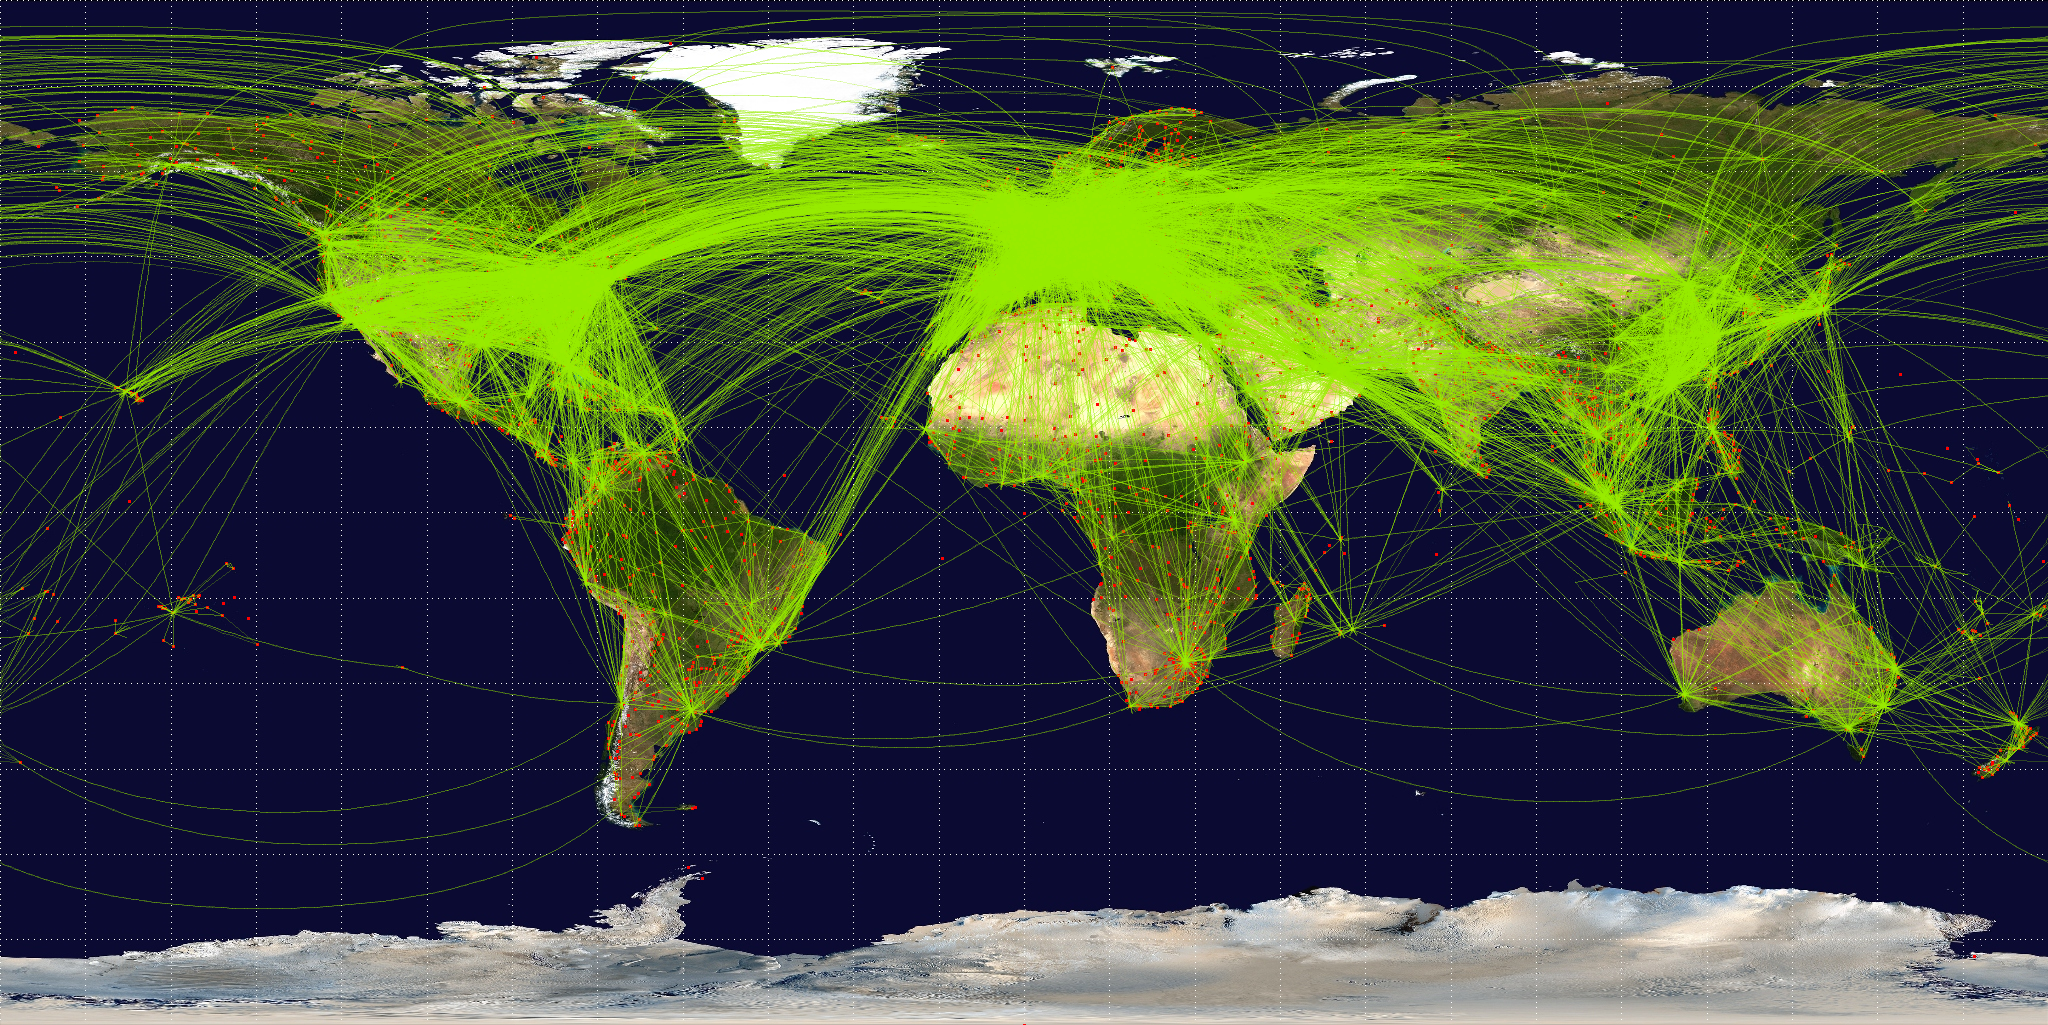
\includegraphics[scale = 0.18]{Pictures/flightpaths.png}
	
	\caption[Popular flight routes]{Popular flight routes, from \cite{Open}}
	\label{fig:flightpaths}
\end{figure} 

The advantages of space-based ADS-B coverage would mainly come from areas where ground-coverage is not possible. For this reason, flight paths that were primarily over land-masses were not considered for analysis. This eliminated the majority of flights originating in the EU and ending in any of Africa, Asia and Australia. Analysis then focussed on flights passing over the Atlantic and Pacific Oceans. These flights were mostly between the United States and Europe, Asia and Australia, as shown in Figure \ref{fig:transoceanicflights}.

\begin{figure}[H]
	\centering
	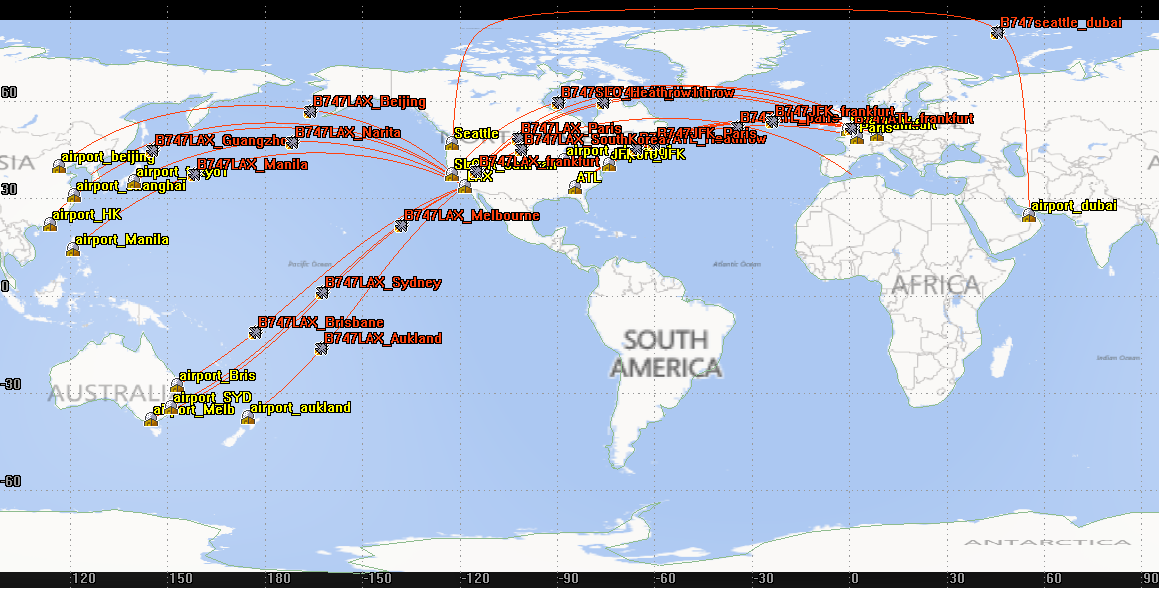
\includegraphics[scale = 0.45]{Pictures/transoceanicflights.png}
	
	\caption{Trans-Oceanic Flight paths, as modelled in STK}
	\label{fig:transoceanicflights}
\end{figure} 

Of these flights, three generalisations were defined and one flight from each generalisation was used for modelling -
\begin{enumerate}
	\item \textbf{North America to Asia} - The path between Los Angeles International Airport (LAX) and Narita airport (NRT) in Tokyo Japan 
	\item \textbf{North America to Europe} - The path between LAX and Heathrow (LHR).
	\item \textbf{North America to Australia} - The path between LAX and Sydney (SYD) International Airport.
\end{enumerate}
These generalisations are highlighted in red Figure \ref{fig:transoceanicGeneralisations}.


\begin{figure}[H]
	\centering
	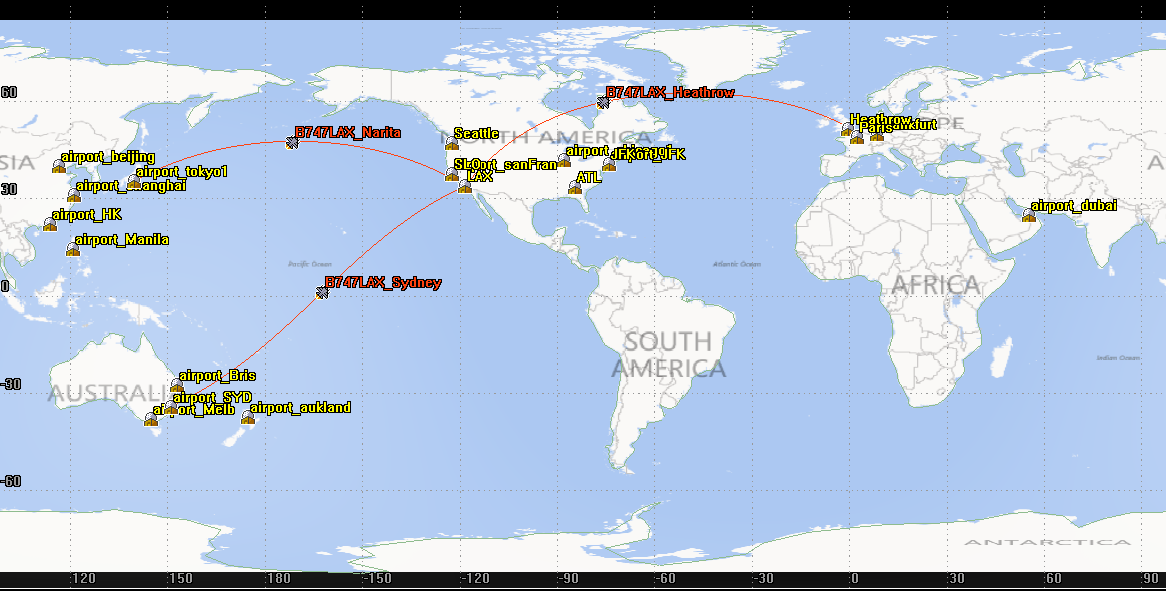
\includegraphics[scale = 0.55]{Pictures/transoceanicGeneralisations.png}
	
	\caption{Generalisations of trans-Oceanic Flight paths used for analysis}
	\label{fig:transoceanicGeneralisations}
\end{figure} 

The performance of a given constellation was determined by examining the ADS-B coverage available for each flight by the parameters outlined in Section \ref{sec:perfMetrics}. The flights were simulated as going continuously back and forth between their two destination airports. The effect of this periodicity is expanded upon in Section \ref{sec:analysis_period}.

\subsection{Input Variables}
The performance metrics presented in Section \ref{sec:perfMetrics} were evaluated against different constellation configurations. Initial tests, discussed later in Section \ref{sec:initial_constel}, ruled out Molniya, geostationary and medium to high earth orbits as practical solutions. The parametric study was then restricted to Low-Earth Orbits, varying orbital parameters from a `reference case'.

\subsubsection{Reference Case} \label{sec:ref_case}
The reference case was chosen to be a constellation of 12 satellites distributed in three circular orbital planes, each with four equispaced satellites. Each orbital plane was inclined at 60 degrees and were at an altitude of 700km above the Earth (a semi-major axis of 7078.14km). The three planes were separated by 120 degrees of Right Angle of Ascending Node (RAAN), starting from 0 degrees for plane one. The four satellites within each plane were separated by true anomalies of 90 degrees. These parameters are summarised in Table \ref{tab:satRefCase}. The ground track of the configuration is shown in Figure \ref{fig:12sat_2d} and the 3D representation is given in Figure \ref{fig:12sat_3d}

\begin{table}[htbp]
  \centering
  \caption{`Reference' constellation configuration}
    \begin{tabular}{lr}
    \toprule
    Parameter & Value\\
    \midrule
    Total number of satellites & 12  \\
    Orbital planes	& 3\\
    Satellites per plane & 4\\
    Separation between planes & 120 deg RAAN \\
    Spacing within a plane & 90 deg true anomaly\\
    Orbit type & Circular, LEO \\
    Semi-major axis & 7078.14km \\
    				&(700km altitude)\\

    \bottomrule
    \end{tabular}%
  \label{tab:satRefCase}%
\end{table}%

\begin{figure}[htbp]
	\centering
	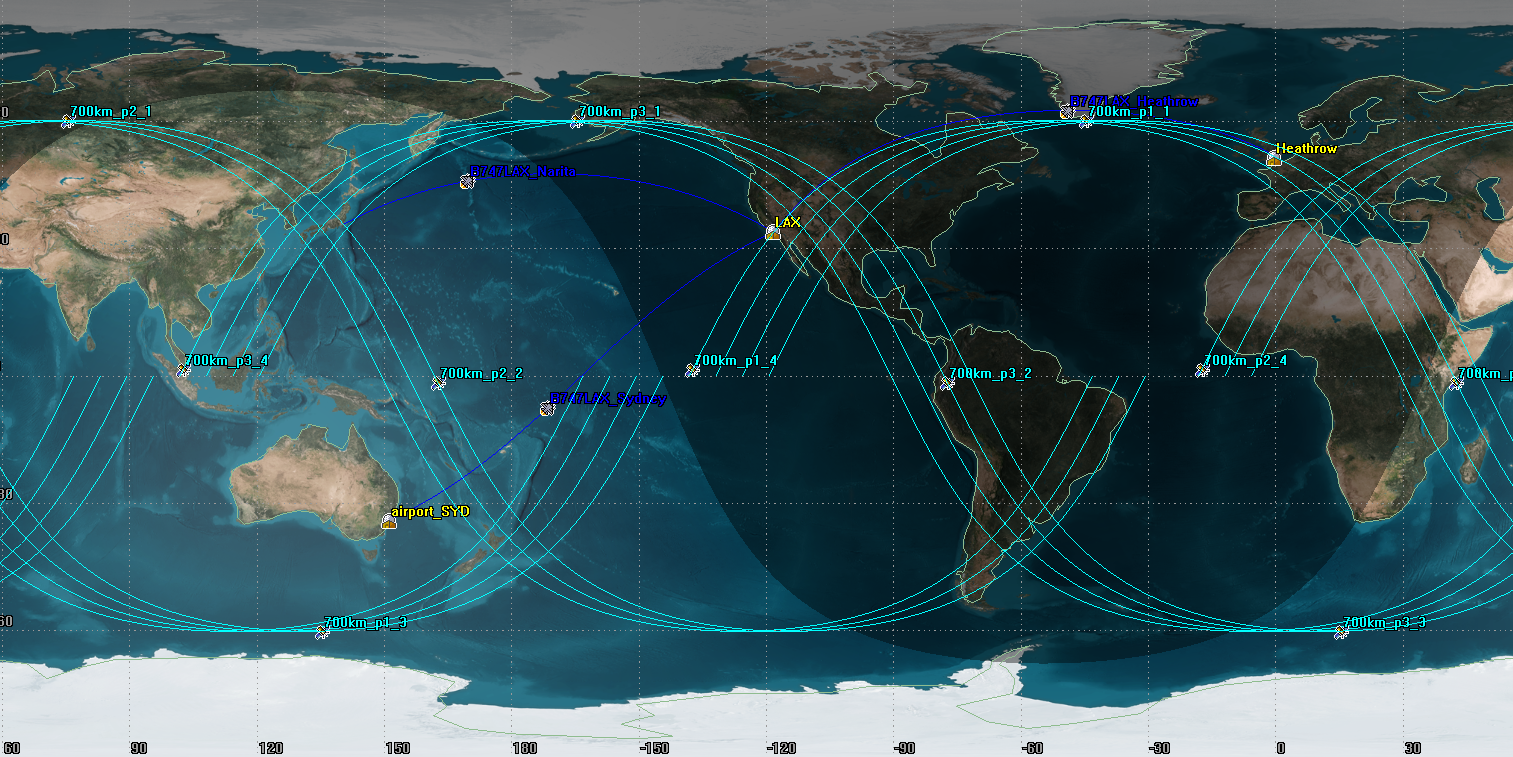
\includegraphics[scale = 0.40]{Pictures/12sat_2d.png}
	
	\caption{Ground track of the 12 satellite reference configuration in STK}
	\label{fig:12sat_2d}
\end{figure} 

\begin{figure}[htbp]
	\centering
	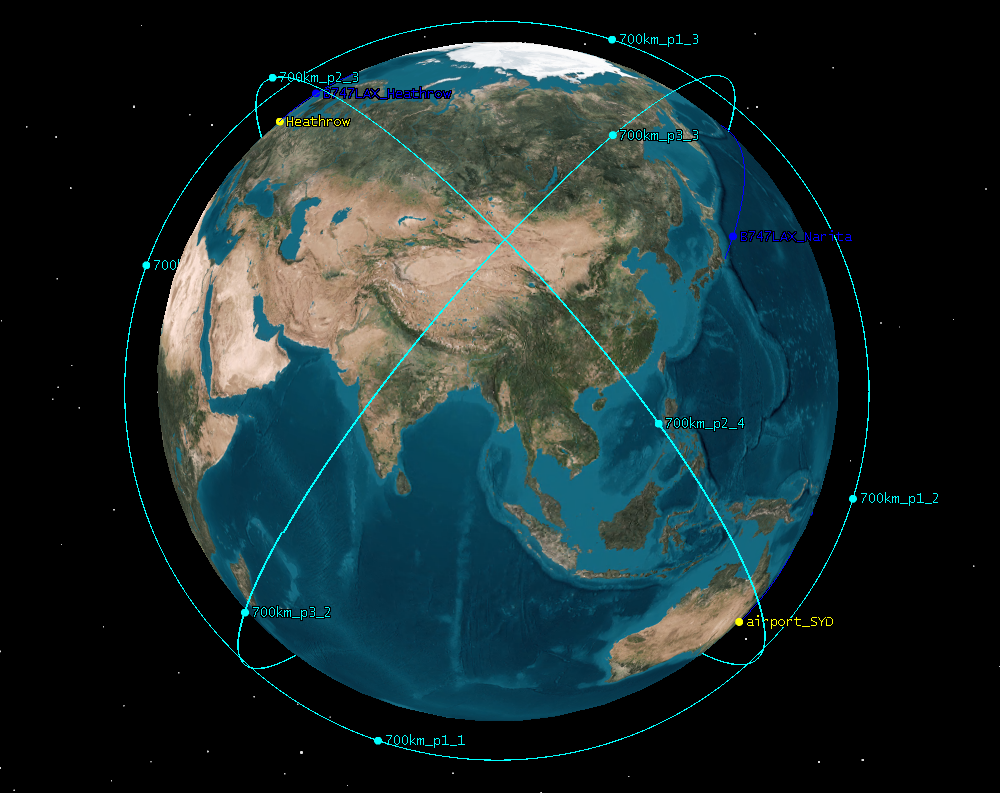
\includegraphics[scale = 0.4]{Pictures/12sat_3d.png}
	
	\caption{3D model of the 12 satellite reference configuration in STK}
	\label{fig:12sat_3d}
\end{figure} 

It was expected that change in inclination, altitude and number of satellites will effect the performance of a given constellation. An increase in altitude would result in an increase in orbital period, but would also increase the receiver footprint of a given satellite with a greater field of view. The change in inclination would vary the maximum and average coverage gap times as the ground traces intersect with the flight paths in different ways.  The change in the number of satellites would change the average and maximum ADS-B coverage gaps, but provide a trade-off with the number of satellites requiring production, maintenance and replacement.

\subsection{Test Cases}
\label{sec:sat_testcases}
From the reference case, inclination, altitude and number of satellites per-plane were varied according to the values presented in Table \ref{tab:satInputParams}. The full table of cases evaluated is given in Appendix \ref{app:all_parameters}.
\begin{table}[H]
  \centering
  \caption{Varying input parameters used for data and analysis}
    \begin{tabular}{lrrr}
    \toprule
    Input Parameter & Minimum & Maximum & Step Size \\
    \midrule
    Altitude & 400km & 800km & 50km  \\
    Satellites per plane & 1 & 6 & 1\\
    Inclination & 30$^\circ$ & 90$^\circ$ & 10$^\circ$ \\
    \bottomrule
    \end{tabular}%
  \label{tab:satInputParams}%
\end{table}%
\subsection{Analysis Period} \label{sec:analysis_period}
Synchronisation and periodicity were taken into account in selecting an analysis period. The discrepancy between air speed of planes (in the order of 250m/s) and the orbital velocity of LEO satellites (in the order of 8km/s) resulted in asynchronous behaviour.  The analysis period was therefore chosen to be long enough to such that - 
\begin{itemize}
	\item The effective ground track for one satellite would form a continuous swath between the latitudes of inclination. The length of period was chosen so that the ground track would repeat over the same global co-ordinates at least once. 
	\item The aggregate results of analysis would accurately take into account all cases where the lack of synchronisation between orbital period and flight time would produce abnormal results. That is, sufficiently many orbital and flight periods are repeated in order to observe an accurate aggregate effect and identify each of the worst-case scenarios.
\end{itemize} 
After initial tests it was found that an analysis period of approximately six days was appropriate. In STK the scenario was analysed between 12:00AM on December 6th, 2013 to 12:00AM December 9th, 2013, $\pm$ 24 hours to allow for varying flight times.

\section{Analysis Tools}
The work carried out used a combination of STK, Matlab and Microsoft Excel in order to simulate, process and display the relevant data. Observations and analysis was carried out based upon the outputs from each of the three steps in the experimental process.
\subsection{STK}
STK version 10.0.2 was used in order to simulate flights, satellite orbits and communication links over the relevant analysis period. The flight paths of interest were chosen according to the process outlined in Section \ref{sec:flight_selection} and the characteristics defined in Section \ref{tab:flightSTKParams} were programmed into STK in order to create the plane and flight models. Each satellite constellation was modelled as a collection of standard satellites, with orbital parameters as specified in Section \ref{sec:sat_testcases}. The STK Communications Toolkit was then used to simulate the ADS-B links between the modelled flights and satellites, outputting data about access times and link budget. The simulation was run continuously for the duration of the analysis period discussed in \ref{sec:analysis_period}. The raw data generated by this model is described in Table \ref{tab:STKData}.

\begin{table}[htbp]
  \centering
  \caption{Raw data generated by STK}
    \begin{tabular}{lp{10cm}}
    \toprule
    Data & Description \\
    \midrule
    Access Times & The start and stop times of periods where a particular flight can access a particular satellite. This is output as \Verb|.csv| files per test of all accesses for the flight and the satellites in the orbit of interest during the test.  \\
    Link Budget & Characteristics of the communication link established during each flight-to-satellite access. Of particular interest is the received isotropic power at the satellite. This is output as \Verb|.csv| files per test of all accesses for the flight and the satellites in the orbit of interest during the test.  \\
    \bottomrule
    \end{tabular}%
  \label{tab:STKData}%
\end{table}%

\subsection{Matlab}
Matlab was used in order to concatenate and sort the data generated by the STK simulation and output the performance data specified in Section \ref{sec:perfMetrics}. The access times \Verb|.csv| files were sorted and concatenated in order to extract the `gap' times where a flight has no access to any satellite. Periods of `access' and `gap' were averaged and the minima and maxima were extracted for further analysis and display. Similarly the link budget \Verb|.csv| files were analysed in Matlab to extract the minimum received isotropic power for each flight.

\subsection{Excel}
Finally, the data outputted from Matlab was imported into Microsoft Excel in order to easily display the data for the analysis of trends and the calculation of the system trade-off decision matrix.
\section{Model Input Data and Assumptions}
Data used in the simulations was researched from official sources was used in order to generate simulations that would closely represent the expected true-to-life situations. 
\subsection{Link Type}
A series of simplifying assumptions were made about the characteristics of the ADS-B links being analysed. The parameters used in the STK link model are summarised in Table \ref{tab:linkParams}. 
% Table generated by Excel2LaTeX from sheet 'Sheet1'
\begin{table}[H]
  \centering
  \caption{Link Parameters used in STK}
    \begin{tabular}{p{3cm}rp{5cm}r}
    \toprule
    \textbf{Parameter} & \textbf{Value} & \textbf{Description} & \textbf{Source} \\
    \midrule
    Transmitter Model & `Simple Transmitter Model' & The transmitter model type used by STK to propagate and analyse link budgets & \cite{STKOnline} \\ \hline
    Equivalent Isotropically Radiated Power (EIRP) & 240W & Power transmitted through an ADS-B antenna assuming zero losses between transponder and antenna & \cite{Garmin2007,Corporation2011,TrigAvionics,BendixKing2013}  \\ \hline
    Bit Error Rate (BER) & $10^{-6}$ & Minimum bit error rate of a link &  \cite{RTCA2013}  \\ \hline
    Modulation Type & `Pulsed Signal' & Type of modulation used in the link &  \\ \hline
    Bandwidth & 8MHz & The bandwidth of an ADS-B Signal &  \cite{RTCA2013}  \\ \hline
    Frequency & 1090MHz & The carrier frequency of ADS-B and Mode S signals &  \cite{STKOnline} \\ \hline
    Receiver Model & `Simple Receiver Model' & The receiver model type used by STK to analyse links from transmitters &  \cite{STKOnline} \\ 
    \bottomrule
    \end{tabular}%
  \label{tab:linkParams}%
\end{table}%

Transmission power was generalised based upon a survey of commercially available transponders \cite{Garmin2007,Corporation2011,TrigAvionics,BendixKing2013} to 240W, transmitted with the assumption that there were insignificant signal losses between the transmitter and antenna. The minimum bit-error rate (BER) was set to $10^6$ bits per second based on the ADS-B  transimission specification released by the RTCA \cite{RTCA2013}. A `pulsed signal' was used in order to model the radar-like behaviour of ADS-B, as suggested by \cite{STKOnline} and no filter was applied to the output. The signal bandwidth was set to 8MHz (+/- 4MHz) as specified by \cite{RTCA2013}. 

These parameters were input to a `Simple Transmitter Model' was used in STK, as the suggested model to use during the system engineering process \cite{STKOnline}. Modelling a more complex transmitter model and defining antenna and propagation type were considered outside the scope of this thesis.

Each of the satellites in the space segment was given a `Simple Receiver Model'. The receiver gain divided by system noise temperature $G/T$ was left unchanged from the default $20K$. Other link parameters would be automatically completed upon analysis of a link with a specified transmitter \cite{STKOnline}. 

\subsection{Flight Characteristics}
Analysis focussed primarily on the performance of ADS-B coverage for a plane during the transoceanic portion of the flight path of interest. Planes within range of an airport would already be serviced by the airport's ground ADS-B receivers. Flights were therefore modelled as single aircraft travelling at a constant cruise speed and altitude between the source and destination airports, ignoring landing and take-off procedures.  

Typical cruise altitudes for commercial airliners range between 30 000 and 40 000 feet. The lower bound of 30 000 feet was chosen in order to maximise the distance travelled by an ADS-B transmission, producing a worst case scenario for signal loss.

The Boeing 747 was chosen as a `typical' commercial transoceanic aircraft, with a cruising speed of 913 km/h. The 747 was chosen after examining a cross section of the typical cruising speeds of popular `long haul' commercial aircraft,  given in Table \ref{tab:flightSpecs}.

% Table generated by Excel2LaTeX from sheet 'Sheet2'
\begin{table}[H]
  \centering
  \caption{Cruising speeds of typical commercial aircraft}
    \begin{tabular}{lrrrr}
    \toprule
    Manufacturer & Model & Speed (km/h) & Speed(km/s) & Source \\
    \midrule
    Boeing & 747-400 & 913   & 0.25361 & \cite{Boeing747}  \\
    Boeing & 777-200 & 1029 & 0.28584 &  \cite{Boeing777} \\
    Boeing & 757-200 & 980 & 0.27222 & \cite{Boeing757}  \\
    Airbus & A380  & 945   & 0.2625 &  \cite{Frawley2014} \\
    \bottomrule
    \end{tabular}%
  \label{tab:flightSpecs}%
\end{table}%

A summary of the aircraft parameters used in STK is given in Table \ref{tab:flightSTKParams}

\begin{table}[H]
  \centering
  \caption{STK Parameters used for each flight model}
    \begin{tabular}{lr}
    \toprule
    Parameter & Value\\
    \midrule
    Altitude & 9.144 km  \\
    	& (30,000 feet)\\
    Speed & 0.2536 km/sec \\
    	& (913 km/h) \\	
    \bottomrule
    \end{tabular}%
  \label{tab:flightSTKParams}%
\end{table}% 

The global co-ordinates for the 4 airports of interest were taken from \cite{Open}, presented in Table \ref{tab:airportCoords}.

\begin{table}[H]
  \centering
  \caption[Airport global co-ordinates]{Airport global co-ordinates, from \cite{Open}.}
    \begin{tabular}{p{4cm}lrrr}
    \toprule
    Airport Name & City & Code & Longitude & Latitude \\
    \midrule
    Los  Angeles International Airport & Los Angeles & LAX   & 33.9425$^\circ$N & 118.4081 $^\circ$W  \\
    London Heathrow Airport & London & LHR   & 51.4775$^\circ$N & 0.4614 $^\circ$W  \\
   	Narita International Airport & Tokyo & NRT   & 35.7653$^\circ$N & 149,3856 $^\circ$E   \\
    Sydney Airport & Sydney & SYD   & 33.9461$^\circ$S & 151,1772 $^\circ$E  \\
    \bottomrule
    \end{tabular}%
  \label{tab:airportCoords}%
\end{table}%

\subsection{Satellite Characteristics}
The standard STK satellite model was used to model each satellite in the test constellations. It was assumed that there would be attitude control aligning the antenna element with the nadir and no active station keeping systems. The STK \Verb|J4Pertubation| orbit propagator was used in order to account for the oblateness of the Earth.
\chapter{Results and Analysis}\label{part:results}
The input parameters detailed in Part \ref{part:exp_method} were simulated in STK and their performance evaluated using tools in Matlab and Microsoft Excel. Initially a set of exotic constellations were tested and ruled out as being impractical and ineffective. Parameters from the reference case detailed in Section \ref{sec:ref_case} were then varied to see the effect on the performance metrics used to define the effectiveness of a space-based ADS-B system. 

\section{Raw Results}
From each simulation in STK, two raw data sets were extracted - a series of access times and the link-budget characterisation for the modelled satellite constellation.

\subsection{Access Times}
Access times were output from STK as tables of access periods. Each access period represented a the period of time where the flight in question was able to establish an RF link with a particular overhead satellite. Access time tables were grouped by satellite by flight analysed. Start and stop times were given in fraction of days from January 1st, 1900. A sample of raw data, taken from the reference case from Section \ref{sec:ref_case} is presented in Table \ref{tab:results_access_sample1}. This data shows the first five accesses between a flight from LAX to Heathrow and two of the satellites in the constellation. All results were concatenated and sorted into for further analysis in Section \ref{sec:data_processing}.
% Table generated by Excel2LaTeX from sheet 'Aircraft-B747LAX_Heathrow-Trans'
\begin{table}[H]
  \centering
  \caption{Sample access data for satellite 1 of the reference case}
    \begin{tabular}{rrrr}
    \toprule
    Access & Start Time (UTCG) & Stop Time (UTCG) & Duration (sec) \\
    \midrule
    1     & 41611.05 & 41611.06 & 945.833 \\
    2     & 41611.12 & 41611.13 & 955.49 \\
    3     & 41611.19 & 41611.20 & 949.135 \\
    4     & 41611.26 & 41611.27 & 958.031 \\
    5     & 41611.33 & 41611.34 & 930.449 \\
    \bottomrule
    \end{tabular}%
  \label{tab:results_access_sample1}%
\end{table}%


\subsection{Link Budget}
Link budget data was sampled by STK every hour. As with the access times, data was grouped per flight per satellite in the constellation. Each sample of data included the transmitted power (EIRP), received frequency, received isotropic power and other link characteristics. A sample of data outputted from STK from one link is given in Table \ref{tab:results_linkbudget_sample1}. This data was taken from the simulation of the reference case from Section \ref{sec:ref_case} and shows the first 10 samples of the link budget data from a communication link between an LAX-Heathrow flight and one of the satellites in the constellation. This data was also concatenated and sorted for further analysis, as presented in Section \ref{sec:data_processing}.


% Table generated by Excel2LaTeX from sheet 'Aircraft-B747LAX_Heathrow-Trans'
\begin{table}[htbp]
  \centering
  \tiny
  \caption{Sample of link budget data from a simulation of a link between a flight and a satellite}
    \begin{tabular}{rrrrrrrrrrr}
    \toprule
    Time & EIRP & Frequency  & Rcvd. Iso. Power & Flux Density  & g/T &  C/No  & Bandwidth  & C/N & Eb/No  & BER \\
    (UTCG)  & (dBW) & (GHz) & (dBW) & (dBW/m$^2$) & (dB/K) & (dB*Hz) & (kHz) & (dB) & (dB) \\
    \midrule
    41611.05 & 23.979 & 1.09  & -139.95 & -117.75 & -114.97 & -26.32 & 8000.00 & -95.36 & -86.32 & 0.50 \\
    41611.05 & 23.979 & 1.09  & -138.93 & -116.72 & -115.56 & -25.88 & 8000.00 & -94.91 & -85.88 & 0.50 \\
    41611.05 & 23.979 & 1.09  & -137.76 & -115.56 & -114.62 & -23.79 & 8000.00 & -92.82 & -83.79 & 0.50 \\
    41611.06 & 23.979 & 1.09  & -136.45 & -114.24 & -111.52 & -19.37 & 8000.00 & -88.40 & -79.37 & 0.50 \\
    41611.06 & 23.979 & 1.09  & -134.96 & -112.76 & -105.35 & -11.71 & 8000.00 & -80.74 & -71.71 & 0.50 \\
    41611.06 & 23.979 & 1.09  & -133.30 & -111.10 & -95.07 & 0.23  & 8000.00 & -68.80 & -59.77 & 0.50 \\
    41611.06 & 23.979 & 1.09  & -131.57 & -109.36 & -80.30 & 16.73 & 8000.00 & -52.30 & -43.27 & 0.50 \\
    41611.06 & 23.979 & 1.09  & -130.10 & -107.89 & -64.44 & 34.06 & 8000.00 & -34.97 & -25.94 & 0.47 \\
    41611.06 & 23.979 & 1.09  & -129.57 & -107.36 & -57.96 & 41.07 & 8000.00 & -27.96 & -18.93 & 0.44 \\
    \bottomrule
    \end{tabular}%
  \label{tab:results_linkbudget_sample1}%
\end{table}%

\section{Data Processing}
\label{sec:data_processing}
\begin{comment}
Raw data was taken from STK, analysed and sorted in Matlab before trend analysis was carried out in Excel.

\subsection{Initial Sorting}
\end{comment}
The raw per-satellite data from STK was combined to create a data set representative of the performance of the constellation in question. A sample of the output from Matlab is given in Table \ref{tab:results_matlab}, with start and stop times given in fraction of days since January 1st, 1990. This sample was taken from the LAX-Heathrow flight simulation with reference case constellation of satellites. It shows rows demonstrating overlapping access times and the resulting calculations.

Rows of access times for all satellites were sorted by access start time. The difference between the access start time of the current row and the access stop time of the previous row was used to calculate the 'gap' time between accesses. In the case of overlapping access times, the difference is negative and discarded (marked in Table \ref{tab:results_matlab} as `N/A'). For these cases, the total `access time' is calculated as the difference between the end of the last calculated gap and the beginning of the current gap. 
% Table generated by Excel2LaTeX from sheet 'Sheet4'
\begin{table}[htbp]
  \centering
  \caption{Calculated access times from Matlab}
    \begin{tabular}{rrrrrrrr}
    \toprule
    Satellite & Access & Access Start & Access  Stop & Access & Gap Start & Gap Stop & Gap \vspace{-3mm} \\
    
    Number & Number & Time & Time & Length (s) & Time & Time & Length(s)\\
    \midrule
    2     & 6     & 41611.38 & 41611.39 & 845.73 & 41611.37 & 41611.38 & 664.42 \\
    1     & 6     & 41611.40 & 41611.41 & N/A  & 41611.39 & 41611.40 & 711.17 \\
    8     & 1     & 41611.41 & 41611.41 & 891.41 & N/A  & N/A  & N/A \\
    4     & 6     & 41611.42 & 41611.43 & N/A  & 41611.41 & 41611.42 & 676.12 \\
    7     & 1     & 41611.42 & 41611.43 & 895.24 & N/A  & N/A  & N/A \\
    3     & 6     & 41611.44 & 41611.44 & N/A  & 41611.43 & 41611.44 & 681.03 \\
    6     & 1     & 41611.44 & 41611.45 & 848.90 & N/A  & N/A  & N/A \\
    2     & 7     & 41611.45 & 41611.46 & N/A  & 41611.45 & 41611.45 & 697.37 \\
    5     & 1     & 41611.45 & 41611.46 & 936.46 & N/A  & N/A  & N/A \\
    1     & 7     & 41611.47 & 41611.48 & N/A  & 41611.46 & 41611.47 & 560.17\\
    \bottomrule
    \end{tabular}%
  \label{tab:results_matlab}%
\end{table}%

\subsection{Statistical Modelling} \label{sec:prob_distro}
The periodicity of concatenated access periods (discarding `N/A' values) was indicative of the number of `discrete' sample points available along a flight. A lower average period of access meant a higher access and update rate for a particular flight path. This higher effective sample rate would allow for potential deviations from a flight path to be detected earlier and with greater resolution.
\begin{comment} 
This is illustrated in Figure \ref{fig:periodicity}.
\begin{figure}[htbp]
	\centering
	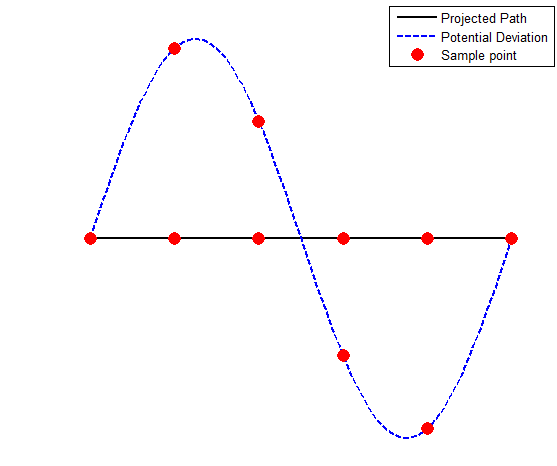
\includegraphics[scale = 0.7]{Pictures/periodicity.png}
	
	\caption{Diagram illustrating how a higher sample rate can detect flight path deviations}
	\label{fig:periodicity}
\end{figure} 
\end{comment}
The access periods for each flight and each constellation were analysed statistically by finding the statistical  model of best fit. This was achieved using the \verb|allfitdist| tool from \cite{sheppard12}. An example of the fitted distribution is given in Figure \ref{fig:allfitdist_Narita}. From the `best fit' model, the mean and standard deviation of the periods were extracted for consideration in the decision matrix.
\begin{figure}[htbp]
	\centering
	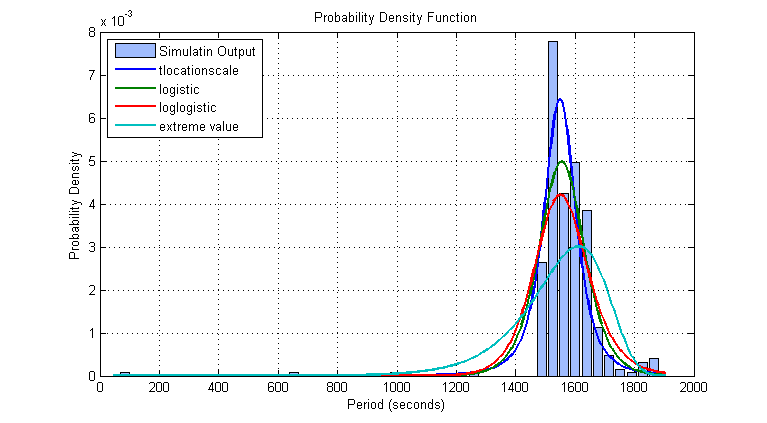
\includegraphics[scale = 0.75]{Pictures/allfitdist_Narita.png}
	
	\caption{Output of allfitdist when applied to the access periods of the LAX-Narita flight using the reference constellation described in Section \ref{sec:ref_case}}
	\label{fig:allfitdist_Narita}
\end{figure} 
\section{Trends and Analysis}
\subsection{Initial Constellation Tests} \label{sec:initial_constel}
During preliminary testing, a Molniya and Geosynchronous orbit were simulated. The results ruled them out as practical orbit options, restricting the bulk of study to LEO satellite constellations.
\subsubsection{Molniya Orbit}
A highly inclined molniya orbit was tested with orbital configuration such that the apogee\footnote{Point at which the satellite is farthest from the Earth} of the orbit occured over the LAX-Heathrow and LAX-Narita flight paths. The ground track of this orbit is shown in Figure \ref{fig:molniya}. It was observed that the satellite would `hang' for long periods of time over the apogee potentially allowing for a longer coverage time. Initial tests yielded a minimum received isotropic power of -161.985 dBW. This was more than 100 times weaker than the worst tested LEO constellation of -140.5 dBW.

\begin{figure}[H]
	\centering
	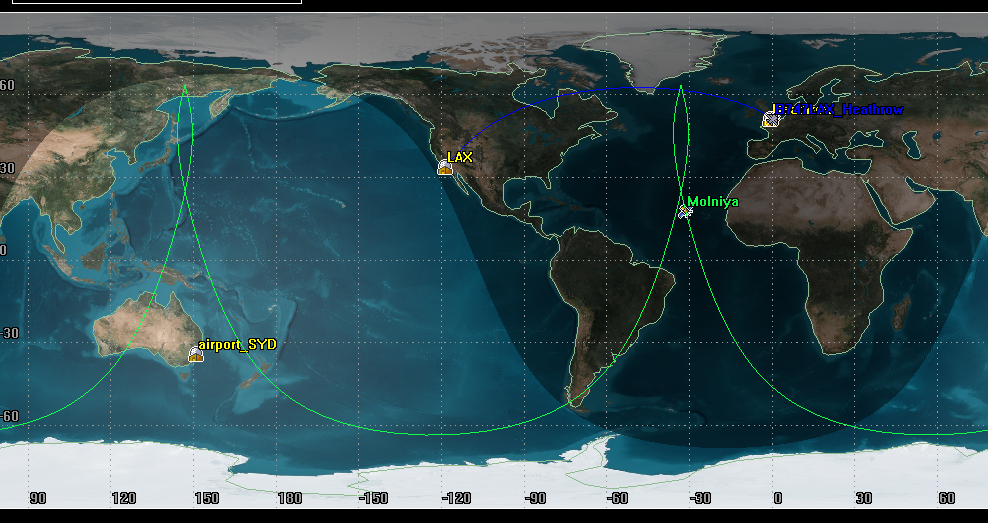
\includegraphics[scale = 0.50]{Pictures/molniya.png}
	
	\caption{Ground track of the tested Molniya orbit}
	\label{fig:molniya}
\end{figure} 

The access times for the LAX-Heathrow flight were evaluated by adding the additional constraint of having a minimum received isotropic power of at least 150.5 dBW (10 times weaker than the worst LEO constellation). This produced a coverage gap fraction of 0.992, meaning that the flight would spend more than 99 percent of the time not being able to communicate with an overhead satellite. This result and the poor signal performance resulted in the family of Molniya orbits being ruled out for further analysis.


\subsubsection{Geosynchronous}
A geosynchronus orbit with was tested with an inclination of 60 degrees and suborbital longitude of -30 degrees in order to place the ground track above the LAX-Heathrow flight. The ground track is given in Figure \ref{fig:geosynch}. The minimum received RX power ranged between -160.3 dBW in the best case and -161.69 in the worse case. This orbit was then dismissed because of the poor performing worst case signal when compared with LEO constellations. 

\begin{figure}[H]
	\centering
	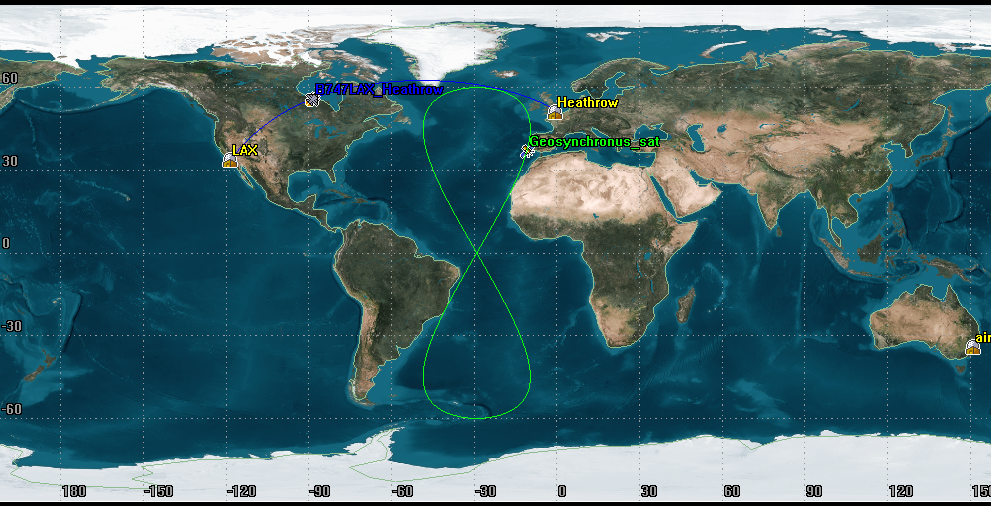
\includegraphics[scale = 0.55]{Pictures/geosynch.png}
	
	\caption{Ground track of the tested Geosynchronous orbit}
	\label{fig:geosynch}
\end{figure} 

\newpage
\subsection{Altitude Variations}
This series of tests involved evaluating the effect of uniformly changing the altitudes of each satellite from the reference case specified in Table \ref{tab:satRefCase} on the performance metrics outlined in Section \ref{sec:perfMetrics}.
\subsubsection{Input Variables}
From the reference case specified in Table \ref{tab:satRefCase}, the altitudes of each satellite were varied between 400km and 800km in 50km steps according to Table \ref{tab:altitudeParams}.

\begin{table}[H]
  \centering
  \caption{Altitude variations used}
    \begin{tabular}{p{2.5cm}rr}
    \toprule
    Case Number & Altitude (km) & Semi-Major Axis (km)\\
    \midrule
    1     & 400   & 6778.14 \\
    2     & 450   & 6828.14 \\
    3     & 500   & 6878.14 \\
    4     & 550   & 6928.14 \\
    5     & 600   & 6978.14 \\
    6     & 650   & 7028.14 \\
    7     & 700   & 7078.14 \\
    8     & 750   & 7128.14 \\
    9     & 800   & 7178.14 \\

    \bottomrule
    \end{tabular}%
  \label{tab:altitudeParams}%
\end{table}%
All other orbital parameters remained constant as per Table \ref{tab:satRefCase}.

It was originally thought that the high number of satellites in the reference constellation was causing a high degree of overlap between coverage from different satellites. This would pollute the observed trend of the access-coverage behaviour. The set of experiments was repeated using a smaller 3 satellite constellation with orbital parameters specified in Table \ref{tab:3sat_config}. The range of altitudes tested was the same as specified in Table \ref{tab:altitudeParams}.
% Table generated by Excel2LaTeX from sheet 'Sheet1'
\begin{table}[htbp]
  \centering
  \caption{Orbital parameters for 3 satellite test}
    \begin{tabular}{rrr}
    \toprule
    Satellite & RAAN  & True Anomaly \\
    \midrule
    1     & 0     & 0 \\
    2     & 120   & 120 \\
    3     & 240   & 240 \\
    \bottomrule
    \end{tabular}%
  \label{tab:3sat_config}%
\end{table}%



\subsubsection{Trends}
The results for altitude variations against the resulting coverage gap fractions, maximum gap period and minimum received signal power are shown in Figures \ref{fig:AltitudeVsCovGap12sat}, \ref{fig:AltitudeVsMaxGap12sat} and \ref{fig:AltitudeVsRxPower12sat} respectively. The results show that the coverage gap fraction and maximum coverage gap become lower with a higher satellite altitude. Similarly the minimum received isotropic power is reduced over time.  The coverage trends for the repeated three-satellite constellation test are given in Figures \ref{fig:AltitudeVsCovGap3sat} and \ref{fig:AltitudeVsMaxGap3sat}, showing the same trends.
\begin{figure}[htbp]
	\centering
	\includegraphics[scale = 0.6]{Pictures/AltitudeVsCovGap12sat.png}
	
	\caption{Coverage gap (as a fraction of total analysis time) as effected by altitude variations. Lower is better}
	\label{fig:AltitudeVsCovGap12sat}
\end{figure} 


\begin{figure}[htbp]
	\centering
	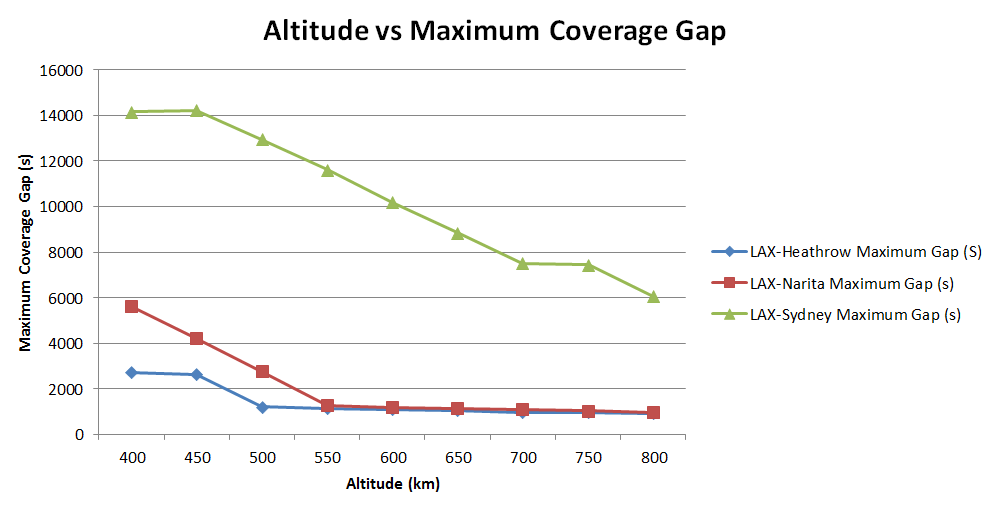
\includegraphics[scale = 0.6]{Pictures/AltitudeVsMaxGap12sat.png}
	
	\caption{Maximum coverage gap as affected by altitude variations. Lower is better}
	\label{fig:AltitudeVsMaxGap12sat}
\end{figure} 

\begin{figure}[htbp]
	\centering
	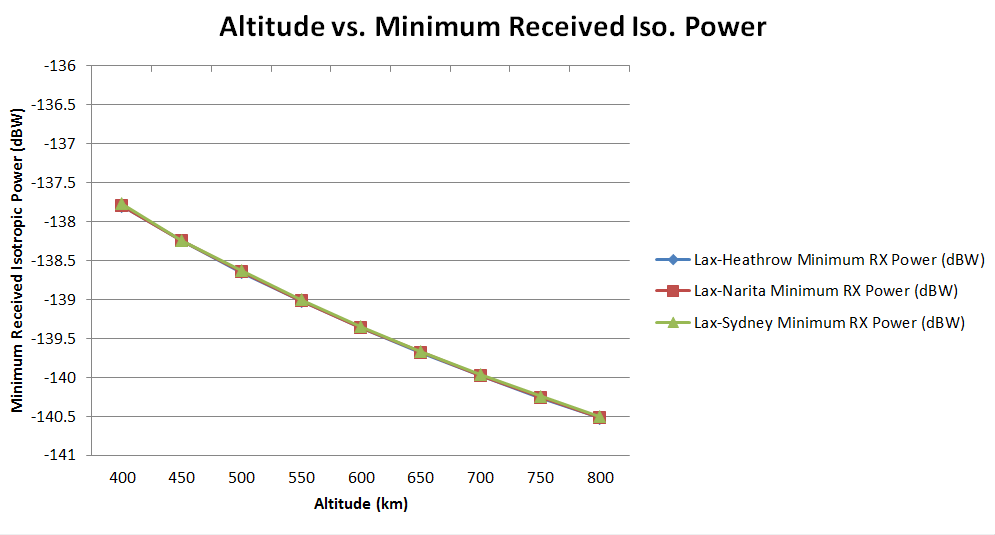
\includegraphics[scale = 0.6]{Pictures/AltitudeVsRxPower12sat.png}
	
	\caption{Minimum received isotropic power as affected by altitude variations. Higher is better.}
	\label{fig:AltitudeVsRxPower12sat}
\end{figure}


\begin{figure}[htbp]
	\centering
	\includegraphics[scale = 0.6]{Pictures/AltitudeVsCovGap3sat.png}
	
	\caption{Coverage gap (as a fraction of total analysis time) as effected by altitude variations with a 3 satellite constellation. Lower is better}
	\label{fig:AltitudeVsCovGap3sat}
\end{figure} 


\begin{figure}[htbp]
	\centering
	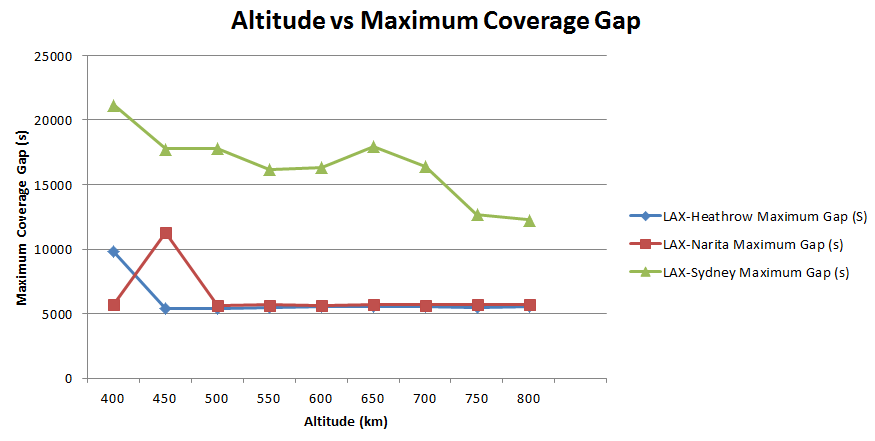
\includegraphics[scale = 0.6]{Pictures/AltitudeVsMaxGap3sat.png}
	
	\caption{Maximum coverage gap as affected by altitude variations retested with a 3 satellite constellation. Lower is better. }
	\label{fig:AltitudeVsMaxGap3sat}
\end{figure} 

\subsubsection{Discussion}
The results for both coverage gap times and received RF power behaved as expected. Satellites at higher altitudes have a greater line of sight range \footnote{The area on Earth within which objects will have a direct line of sight toward a satellite, allowing for a simple RF link to be made.} increasing the probability with which any one flight could be `seen' by a satellite. The difference in orbital period between the extremes of altitude (1 hour and 32.5 minutes at 800km against 1 hour and 42.9 minutes at 400 km) was less than 10\% and had minimal effect on the periodicity of access times. The net effect is the observed increase in coverage time and decrease of coverage `gaps' for any given flight path. The trends observed in the coverage-access times for the three-satellite test shown in Figures \ref{fig:AltitudeVsCovGap3sat} and \ref{fig:AltitudeVsMaxGap3sat} matched those quite closely with those seen in the reference case with 12 satellites. This indicated that the number of satellites did not affect the trend observed in either case

There was a significant observed difference in coverage gaps for the flights between LAX and Sydney and LAX and Heathrow or Narita. The maximum coverage gaps for LAX-Sydney were worse by one order of magnitude of time, as is shown in Figure \ref{fig:AltitudeVsMaxGap12sat}. This is due to the fact that 60 degree inclination of the satellites resulted in ground tracks that were almost coincident with the flight paths between LAX and Narita or Heathrow, as can be seen in Figure \ref{fig:12sat_60deg_flightPaths}. The geometry of the ground tracks was not optimised for the flight path between LAX and Sydney, resulting in a less desirable maximum coverage gap.

\begin{figure}[htbp]
	\centering
	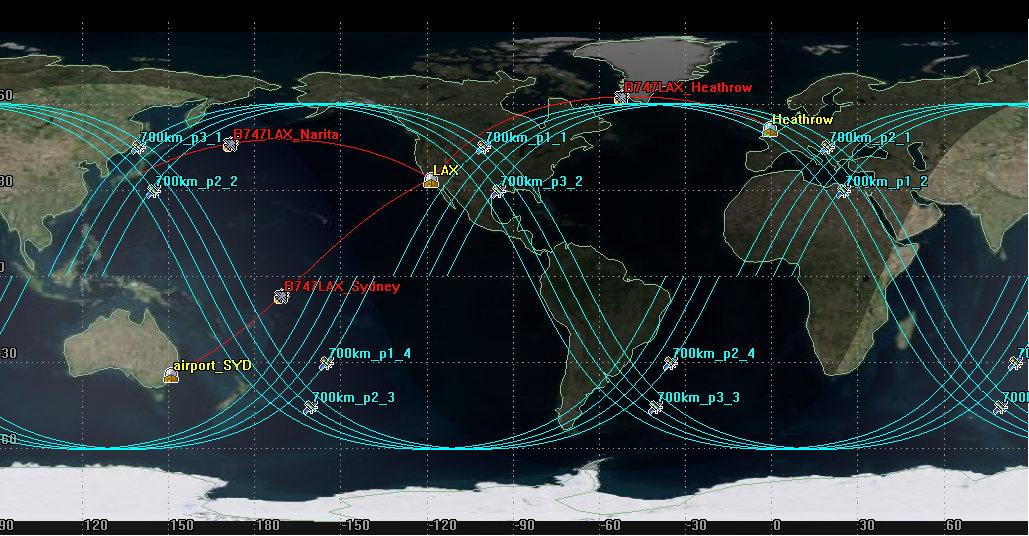
\includegraphics[scale = 0.6]{Pictures/12sat_60deg_flightPaths.png}
	
	\caption{Ground track of satellites inclined at 60 degrees, shown with the test flight paths}
	\label{fig:12sat_60deg_flightPaths}
\end{figure} 

Despite the increased access time at higher altitudes, however, a significant drop in received signal strength is observed between 400km and 800km altitude. There was an expected drop due to the increased distance and subsequent increased free-space path loss of any electromagnetic wave.  The minimum received isotropic power is optimised at 400km, with a measurement of -137.8 dBW and is the least optimised at 800km with a measurement of -140.5 dBW. This is a difference of 2.7 dBW, meaning that from 400km altitude to 800km altitude, the raw signal power has been reduced by a factor of 1.86. This will affect ADS-B detectability as weaker signals will be harder to detect and process. The effect of this on the performance of the system is evaluated later in Section \ref{sec:decision_matrix}.

The minimum trigger threshold level for an ADS-B receiver class R3 (Extended) as specified by the RTCA is set at -84 dBm \cite{RTCA_MODE_S} or -114 dBW. This is already well above that possible with the standard transmitter-receiver model at 400 km altitude. 


  
 
\newpage
\subsection{Inclination Variations}
This series of tests involved evaluating the effect of uniformly changing the inclination of each satellite from the reference case specified in Table \ref{tab:satRefCase} on the performance metrics outlined in Section \ref{sec:perfMetrics}.
\subsubsection{Input Variables}
From the reference case specified in Table \ref{tab:satRefCase}, the inclinations of each satellite were varied between 30 degrees and 90 degrees in 10 degree steps according to Table \ref{tab:inclinationParams}.

\begin{table}[H]
  \centering
  \caption{Inclination variations used}
    \begin{tabular}{p{2.5cm}r}
    \toprule
    Case Number & Inclination (degrees) \\
    \midrule
    1     & 30    \\
    2     & 40  \\
    3     & 60   \\
    4     & 70 	\\
    5     & 80    \\
    6     & 90   \\
    \bottomrule
    \end{tabular}%
  \label{tab:inclinationParams}%
\end{table}%
All other orbital parameters remained constant as per Table \ref{tab:satRefCase}. The ground tracks of the constellation inclined at 30 degrees, 60 degrees and 90 degrees is shown in Figures \ref{fig:12sat_30deg}, \ref{fig:12sat_60deg} and \ref{fig:12sat_90deg} respectively.
\begin{figure}[H]
	
	\begin{subfigure}[b]{\textwidth}
	\centering
	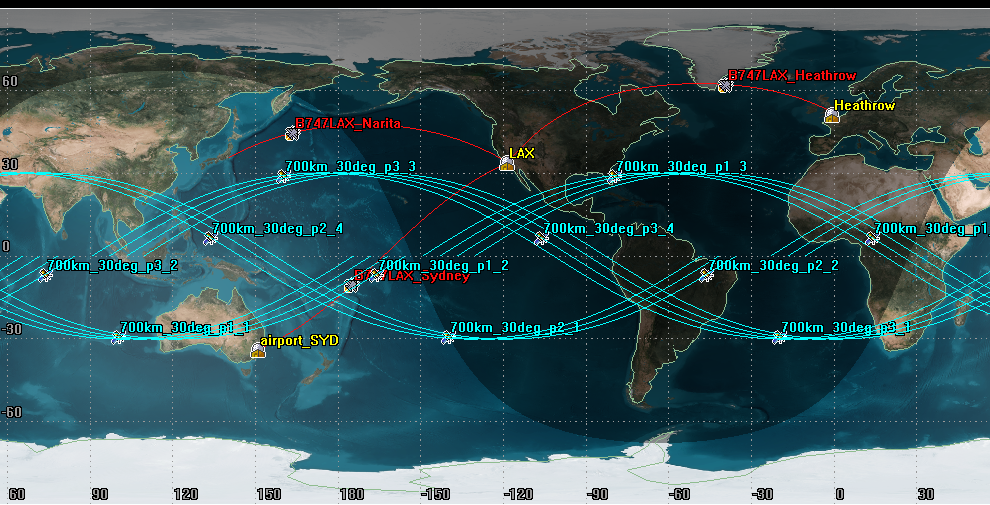
\includegraphics[scale = 0.45]{Pictures/12sat_30deg.png}
	
	\caption{Ground track of satellites inclined at 30 deg (Case 1)}
	\label{fig:12sat_30deg}
	\end{subfigure}
	
	\begin{subfigure}[b]{\textwidth}
	\centering
	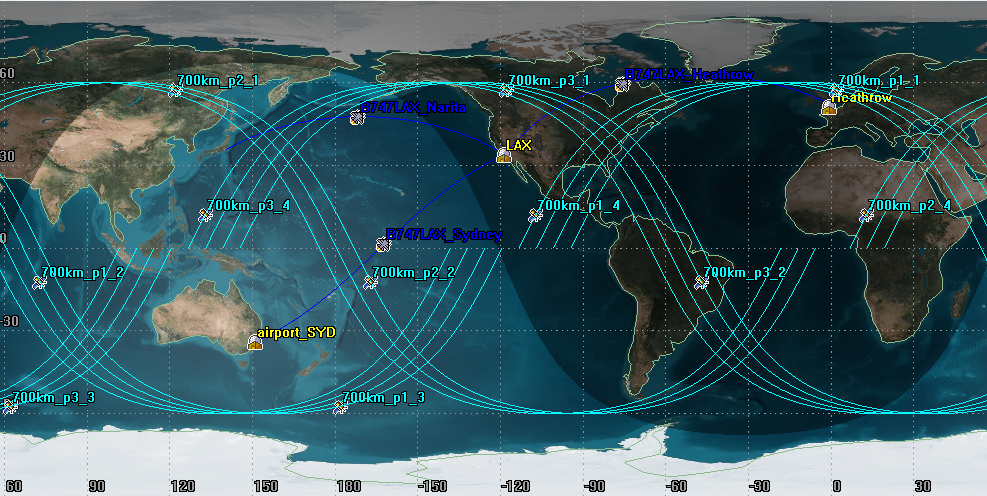
\includegraphics[scale = 0.45]{Pictures/12sat_60deg.png}
	
	\caption{Ground track of satellites inclined at 60 deg (Case 3)}
	\label{fig:12sat_60deg}
	\end{subfigure}
		
	
	\begin{subfigure}[b]{\textwidth}
	\centering
	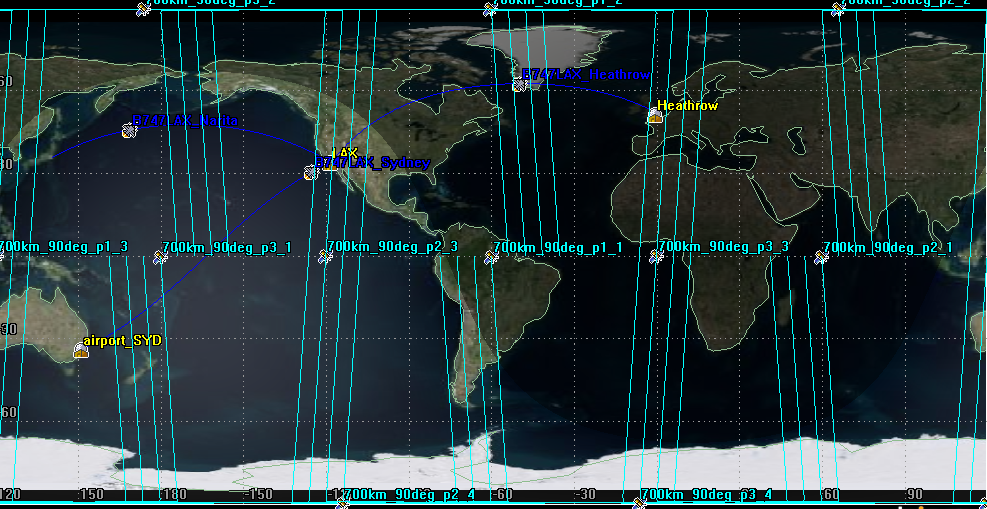
\includegraphics[scale = 0.45]{Pictures/12sat_90deg.png}
	
	\caption{Ground track of satellites inclined at 90 deg (Case 6)}
	\label{fig:12sat_90deg}
	\end{subfigure}
	
	\caption{Ground tracks of constellations inclined between 30 degrees and 90 degrees}
\end{figure} 

\subsubsection{Trends}
The results for inclination variations against the resulting coverage gap fractions, maximum gap period and minimum received signal power are shown in Figures \ref{fig:InclinationVsCovGap12sat}, \ref{fig:InclinationVsMaxGap12sat} and \ref{fig:InclinationVsRxPower12sat} respectively. Each parameter behaved differently for each flight.
\begin{figure}[htbp]
	\centering
	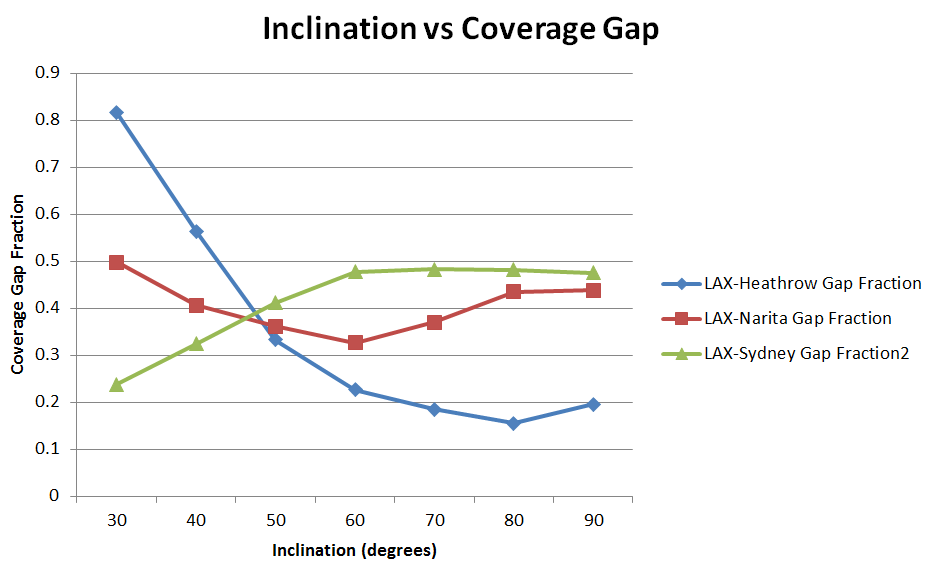
\includegraphics[scale = 0.6]{Pictures/InclinationVsCovGap12sat.png}
	
	\caption{Coverage gap (as a fraction of total analysis time) as effected by inclination  variations. Lower is better}
	\label{fig:InclinationVsCovGap12sat}
\end{figure} 


\begin{figure}[htbp]
	\centering
	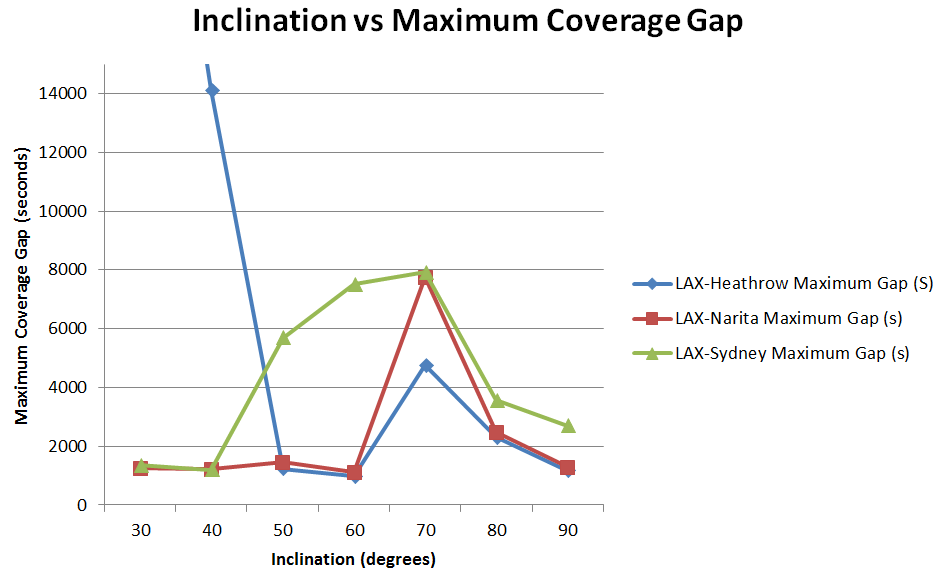
\includegraphics[scale = 0.6]{Pictures/InclinationVsMaxGap12sat.png}
	
	\caption{Maximum coverage gap as affected by altitude variations. Lower is better.}
	\label{fig:InclinationVsMaxGap12sat}
\end{figure} 

\begin{figure}[htbp]
	\centering
	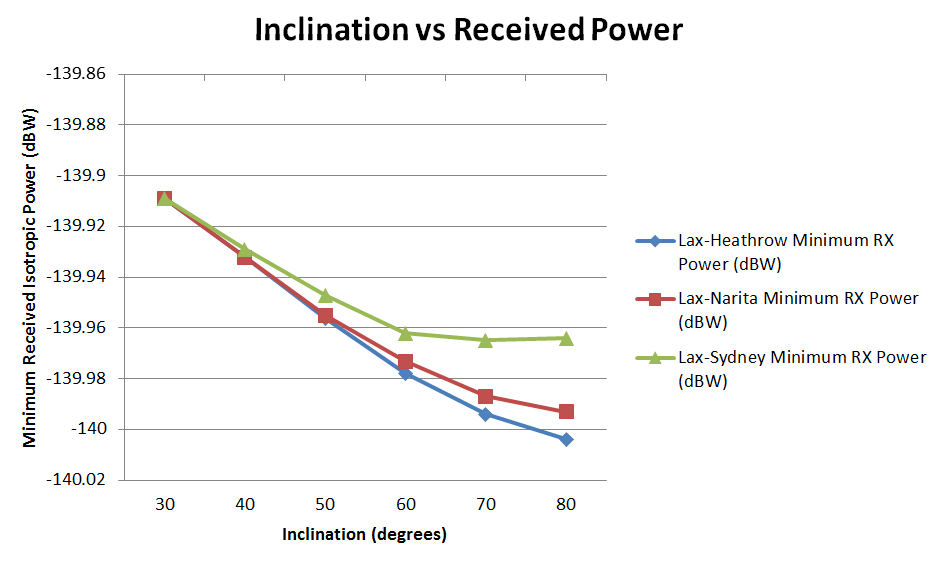
\includegraphics[scale = 0.6]{Pictures/InclinationVsRxPower12sat.png}
	
	\caption{Minimum received isotropic power as affected by inclination variations. Higher is better.}
	\label{fig:InclinationVsRxPower12sat}
\end{figure}
\subsubsection{Discussion}
At lower inclinations, the ground tracks of the satellite have a significant amount of coincidence with the flight path between LAX and Sydney, as seen in Figure \ref{fig:12sat_30deg}. This results in the LAX-Sydney flight path having an optimised maximum coverage time and coverage fraction at 30 degrees inclination as can be seen on Figures \ref{fig:InclinationVsCovGap12sat} and \ref{fig:InclinationVsMaxGap12sat}. Increasing inclinations resulted in a higher coverage gap ratio, before settling at 60 degrees and remaining constant through to 90 degrees.

The relatively high inclination of the LAX-Heathrow flight path resulted in poor coverage performance with the constellation at low inclinations. At low inclinations there were few opportunities for line of sight to be established between the LAX-Heathrow flight, with access periods only occurring when satellites reached high latitudes at the same time as the flight was at a low latitude. The resulting maximum gap (not shown in Figure \ref{fig:InclinationVsMaxGap12sat} for scale purposes) was 29 866 seconds (8 hours and 18 minutes) - more than half the duration of the flight. The aggregate result also yielded a poor coverage gap fraction performance below 50 degrees, as seen in Figure \ref{fig:InclinationVsCovGap12sat}. The effect sharply decreased with higher inclinations, with coverage gaps lowering to an acceptable level after 50 degrees.

All flight paths observed a spike in maximum coverage gap time with satellites inclined at 70 degrees, as seen in Figure \ref{fig:InclinationVsMaxGap12sat}. This occurred due to the geometry of the constellation and the effect of the Earth's rotation under the constellation. Figure \ref{fig:70_deg_precess_1_edited} shows that the effective width between the two orbital planes of the satellite is quite high, creating an effective radio `dead zone' in which the pictured plane cannot access a satellite. Although the plane continues to travel out of the `dead zone', the rotation of the Earth underneath the constellation moves the position of the plane back into the `dead zone', as demonstrated in  Figure \ref{fig:70_deg_precess_2_edited}. At inclinations of 80 degrees and 90 degrees this effect is mediated by the changing geometry and intersections between satellite ground tracks and flight paths, resulting in more acceptable coverage gaps.

There is relatively little change in the minimum received isotropic powers, with values ranging between -139.9 dBW and -140.02 dBW as seen in Figure \ref{fig:InclinationVsRxPower12sat}. The observed trend occurs due to the satellite having a higher chance of being `directly overhead' with higher inclinations, resulting in a shorted free-path propagation distance for the ADS-B signal. However this effect was quite small, only resulting in a net change of 0.12 dBW across the experimented range.

\begin{figure}[htpb]
	\centering
	\begin{subfigure}[b]{0.6\textwidth}
	
	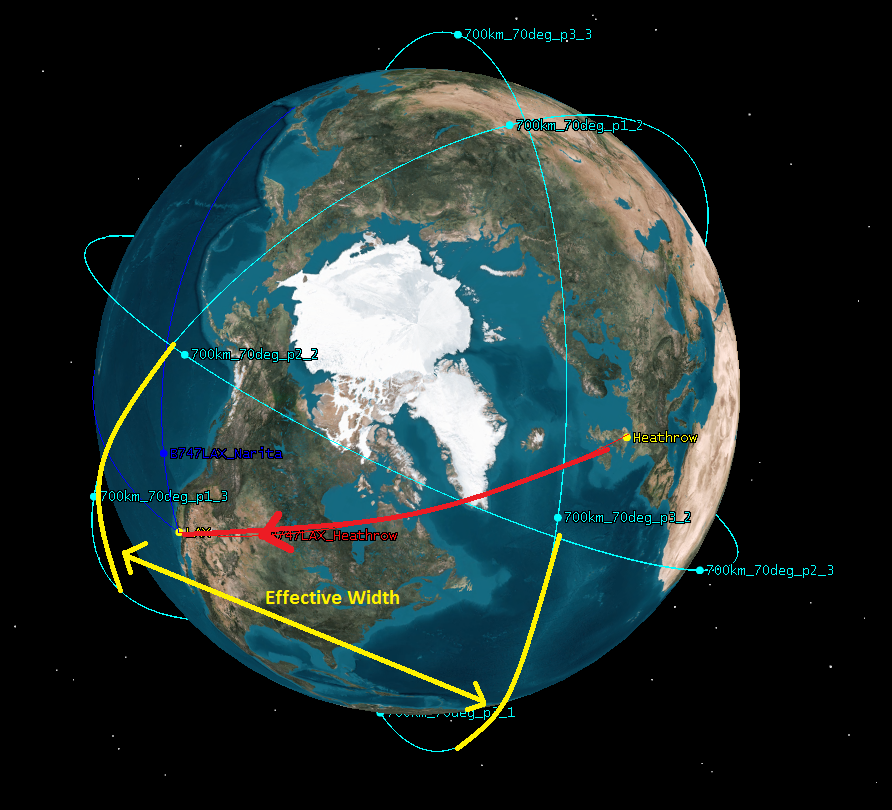
\includegraphics[width=\textwidth]{Pictures/70_deg_precess_1_edited.png}
	
	\caption{Flight initially in `dead zone' of no ADS-B access between planes}
	\label{fig:70_deg_precess_1_edited}
	\end{subfigure}
	
	\begin{subfigure}[b]{0.6\textwidth}
	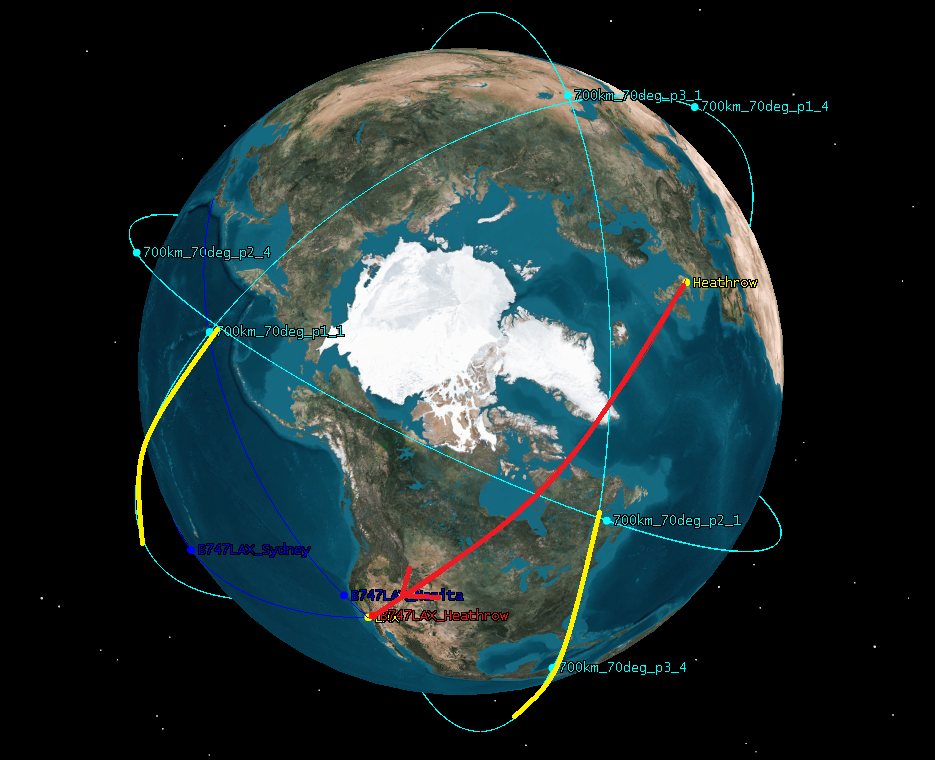
\includegraphics[width=\textwidth]{Pictures/70_deg_precess_2_edited.png}
	
	
	\caption{Rotation of Earth eastward keeps the flight in the `dead zone' for an extended period of time}
	\label{fig:70_deg_precess_2_edited}
	\end{subfigure}
		
	
	\caption{Flight in `dead zone' between satellite planes, inclined at 70 degrees. View from North Pole}
\end{figure} 
\newpage
\subsection{Satellite Number Variations}
This series of tests involved evaluating the effect of changing the number of satellites in the constellation on the performance metrics outlined in Section \ref{sec:perfMetrics}. The same three-plane orbital configuration was kept from Table \ref{tab:satRefCase}, whilst the number of satellites per-plane were changed. 
\subsubsection{Input Variables}
From the reference case specified in Table \ref{tab:satRefCase}, the number of satellites per each of the 3 planes were varied between 1 and 6 according to Table \ref{tab:perPlaneParams}.

\begin{table}[H]
  \centering
  \caption{Number of satellite variations used}
    \begin{tabular}{p{2.5cm}rr}
    \toprule
    Case Number & Satellites per plane & Total Satellites \\
    \midrule
    17    & 1     & 3 \\
    18    & 2     & 6 \\
    19    & 3     & 9 \\
    20    & 4     & 12 \\
    21    & 5     & 15 \\
    22    & 6     & 18 \\

    \bottomrule
    \end{tabular}%
  \label{tab:perPlaneParams}%
\end{table}%
All other orbital parameters remained constant as per Table \ref{tab:satRefCase}.

\subsubsection{Trends}
The results for satellite number variations against the resulting coverage gap fractions, maximum gap period and minimum received signal power are shown in Figures \ref{fig:PerPlaneVsCovGap12sat}, \ref{fig:PerPlaneVsMaxGap12sat} and \ref{fig:PerPlaneVsRxPower12sat} respectively. Generally it was seen that increasing the number of satellites per plane decreased the coverage gaps, whilst the minimum received RF power remained the same
\begin{figure}[H]
	\centering
	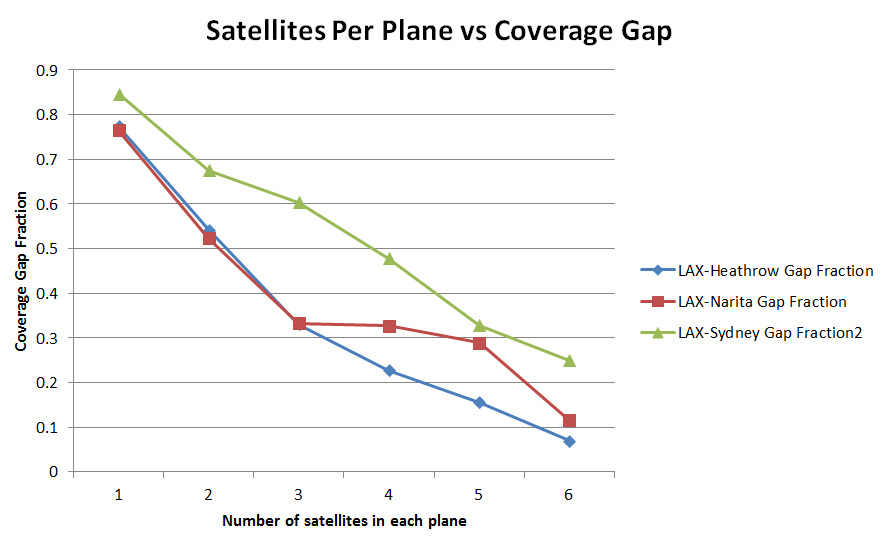
\includegraphics[scale = 0.6]{Pictures/PerPlaneVsCovGap12sat.png}
	
	\caption{Coverage gap (as a fraction of total analysis time) as effected by number of satellites per plane. Lower is better}
	\label{fig:PerPlaneVsCovGap12sat}
\end{figure} 

\begin{figure}[H]
	\centering
	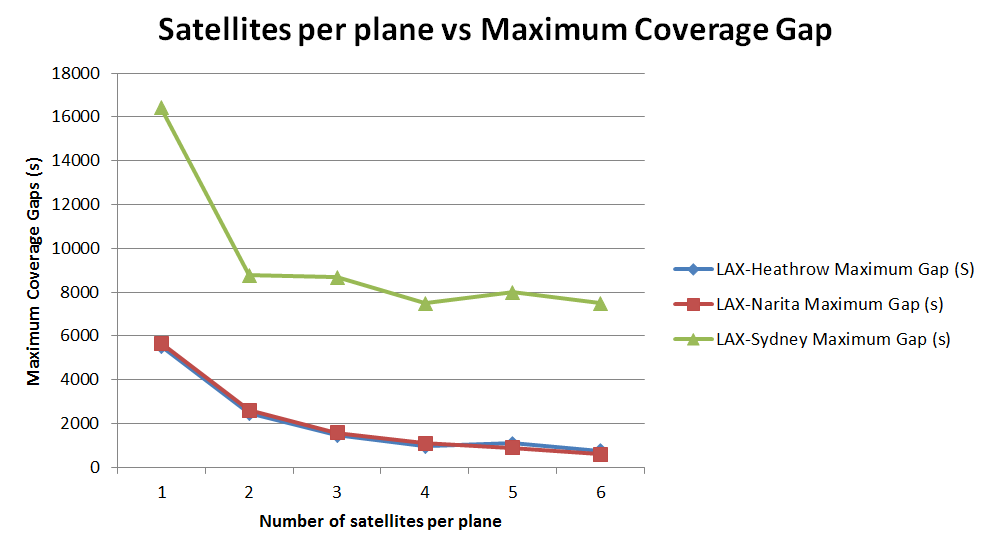
\includegraphics[scale = 0.6]{Pictures/PerPlaneVsMaxGap12sat.png}
	
	\caption{Maximum coverage gap as affected by number of satellites per plane. Lower is better.}
	\label{fig:PerPlaneVsMaxGap12sat}
\end{figure} 

\begin{figure}[H]
	\centering
	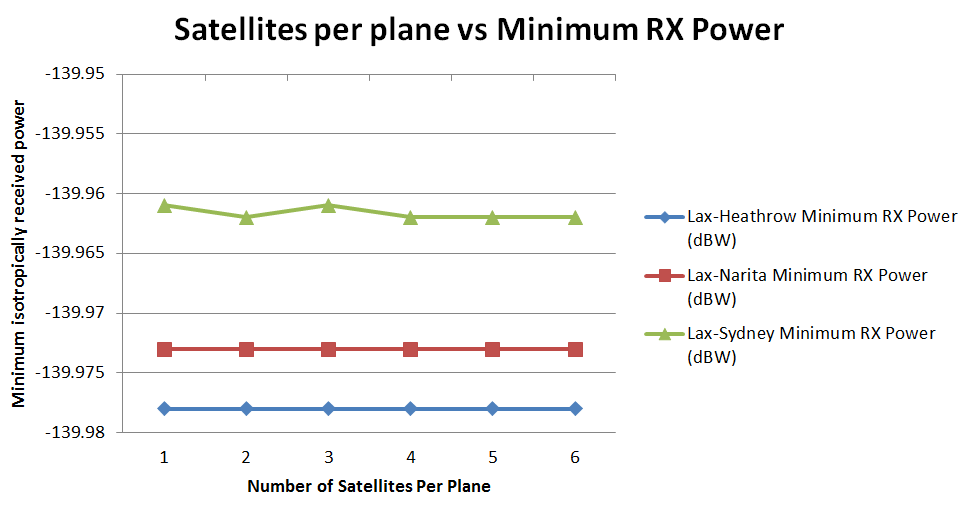
\includegraphics[scale = 0.6]{Pictures/PerPlaneVsRxPower12sat.png}
	
	\caption{Minimum received isotropic power as affected by number of satellites per plane. Higher is better.}
	\label{fig:PerPlaneVsRxPower12sat}
\end{figure}

\subsubsection{Discussion}
As expected, increasing the number of satellites increased the coverage times available for each flight. Figures \ref{fig:PerPlaneVsCovGap12sat} and \ref{fig:PerPlaneVsMaxGap12sat} show that a higher number of satellites results in less coverage gaps. A higher number of satellites per plane increased the probability with which a given flight was able to see at least one satellite, and also increased the revisit time for a given area on the Earth. The number of satellites in the constellation did not affect the minimum received RF power, as seen in the flatness of Figure \ref{fig:PerPlaneVsRxPower12sat}.

Despite the net beneficial effect on the ADS-B system, the number of satellites needs to be weighed against the cost and maintenance. Increasing the number of satellites did increase the effectiveness of the space based ADS-B coverage constellation. However a higher number of satellites will require an increased launch and maintenance cost, especially when considering the need to distribute the satellites evenly and potential replacement at end of life.


 

\section{Access Periodicity} \label{sec:periodicity_stats}
The distributions of coverage periods for all constellations tested were strongly modal, with the majority having one dominant mode. Figure \ref{fig:allfitdist_Heathrow}, from the reference constellation observing the LAX-Heathrow flight, shows a typical distribution. The periods shown all fall within a tight band around the mean, with some outliers and modes to the left and right of the mean. After applying \verb|allfitdist| \cite{sheppard12}, it was found that the Student's t distribution with a location and scale transformation applied, as shown in Figure \ref{fig:allfitdist_Heathrow}. An analysis of the Student's t distribution is given in Appendix \ref{sec:stats}.

\begin{figure}[htbp]
	\centering
	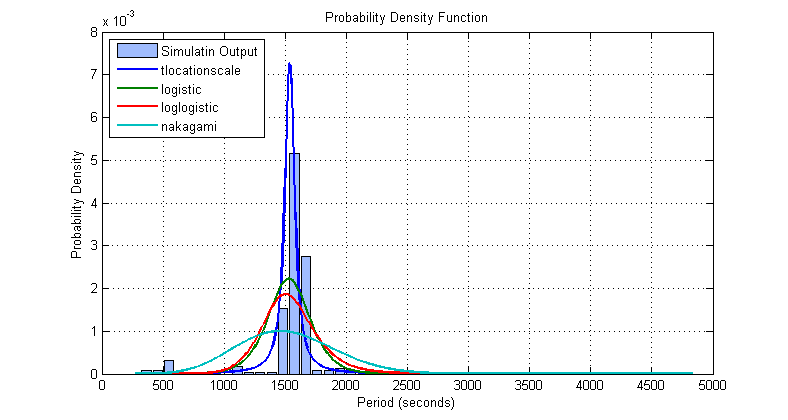
\includegraphics[scale = 0.85]{Pictures/allfitdist_Heathrow.png}
	
	\caption{Fitted distributions of the periodicity of Access times for the LAX-Heathrow flight from the reference constellation. }
	\label{fig:allfitdist_Heathrow}
\end{figure} 
For constellations with more than 12 satellites, the extracted parameters from \verb|allfitdist| yielded values for the degrees of freedom, $\nu$, for which the variance is undefined. Empirically, this was observed as the case if the band of most probable periods was too narrow for analysis using the Student's t distribution as the model. In these cases, the narrow variance was considered desirable and so for the purposes of comparative analysis, the `variance' score in the weighted decision matrix was given the highest score, 10.

It was found that for constellations with a lower number of satellites, there was less of a dominant node and more of an even spread of distributions. Figure \ref{fig:allfitdist_Heathrow6sat} shows the histogram for a six-satellite constellation, showing a larger spread of results. In these cases, \verb|allfitdist| yielded different distributions of best fit, as shown in Figure \ref{fig:allfitdist_Heathrow6sat}. Although these fits are not exact, the extracted variance value was considered a good indicator of comparative variance in periodicity. The standard deviations from these distributions were extracted computationally


\begin{figure}[htbp]
	\centering
	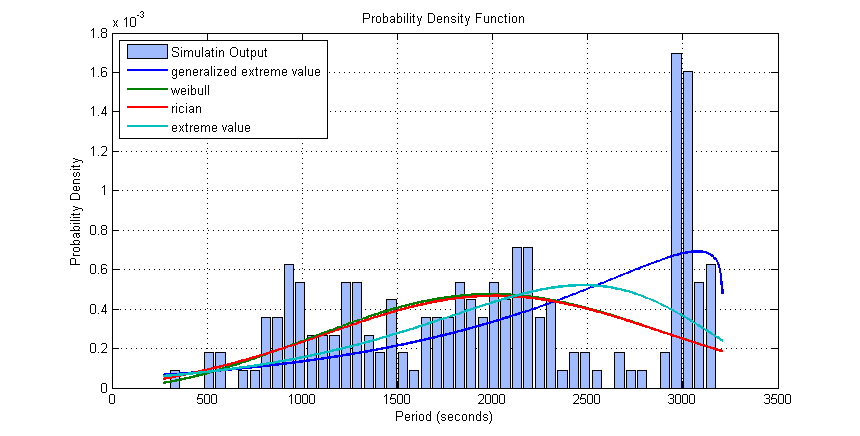
\includegraphics[scale = 0.8]{Pictures/allfitdist_Heathrow6sat.png}
	
	\caption{Fitted distributions of the periodicity of Access times for the LAX-Heathrow flight from the reference constellation. }
	\label{fig:allfitdist_Heathrow6sat}
\end{figure} 

\section{Weighted Decision Matrix}
\label{sec:decision_matrix}
The results from Part \ref{part:results} were collated for numerical comparative analysis using a weighted decision matrix. The results of each performance parameter were linearised to provide scores between 1-10. Weights were applied to each score according to the importance of the parameter to the effectiveness of a space-based ADS-B system. An aggregate score for a constellation was summed from each of the weighted scores and this was used to numerically compare different the different constellations tested.

\subsection{Parameter Weight Matrix}
Each of the four performance metrics described in Section \ref{sec:perfMetrics} were considered differently for each of the tested flight paths detailed in Section \ref{sec:flight_selection}. In addition to these, total number of satellites was also considered for evaluation of overall cost of the system. The parameters used in the weighted decision matrix are given in Table \ref{tab:parameters}

% Table generated by Excel2LaTeX from sheet 'weights'
\begin{table}[htbp]
  \centering
  \caption{Parameters used to evaluate constellation effectiveness}
    \begin{tabular}{lp{5cm}p{6cm}r}
    \toprule
    Flight Path & Parameter & Score Calculation Method & Weight \\
    \midrule
    All   & Number of Satellites & Simple Linearisation - Down  & 10\\
    LAX - Heathrow & Fraction of coverage gap to total time analysed & Simple Linearisation - Down & 20 \\
    LAX - Heathrow & Average Period & Pass-Fail Linearisation  & 10\\
    LAX - Heathrow & Periodicity Deviation & Pass-Fail Linearisation & 5 \\
    LAX - Heathrow & Maximum coverage gap time & Simple Linearisation - Down & 10 \\
    LAX - Heathrow & Minimum Received RX Power & Simple Linearisation - Up & 15 \\
    LAX - Narita & Fraction of coverage gap to total time analysed& Simple Linearisation - Down & 20 \\
    LAX - Narita & Average Period & Pass-Fail Linearisation & 10 \\
    LAX - Narita & Periodicity Deviation & Pass-Fail Linearisation & 5  \\
    LAX - Narita & Maximum coverage gap time & Simple Linearisation - Down & 10 \\
    LAX - Narita & Minimum Received RX Power & Simple Linearisation - Up & 15 \\
    LAX - Sydney & Fraction of coverage gap to total time analysed  & Simple Linearisation - Down & 20 \\
    LAX - Sydney & Average Period & Pass-Fail Linearisation & 10\\
    LAX - Sydney & Periodicity Deviation & Pass-Fail Linearisation & 5 \\
    LAX - Sydney & Maximum coverage gap time & Simple Linearisation - Down & 10\\
    LAX - Sydney & Minimum Received RX Power & Simple Linearisation - Up & 15\\
    \bottomrule
    \end{tabular}%
  \label{tab:parameters}%
\end{table}%

The weights were applied as shown in Table \ref{tab:parameters} subjectively, representing one particular design philosophy. Each flight path was weighted equally in favour evaluating each constellation without geographical bias. Fraction of coverage gap was determined to be the strongest factor as a higher score would ease the system requirements of a number of key factors, including signal collision avoidance and raw samples available. This was followed by minimum received RX power, which would be a defining system requirement for a space based ADS-B sensor. Satellite number and periodicity were less important as CubeSats are relatively cheap to launch and the effect of periodicity can be offset by having a higher access-coverage ratio. 

\subsection{Score Calculation}
  
\subsubsection{Simple Linearisation}
In order to simplify numerical analysis, the numerical results (other than periodicity) from each of experiments conducted in Part \ref{part:results} were linearised between minimum and maximum values. The direction of linearisation was adjusted such that a higher score meant a more favourable result. In the case of maximum, average and fraction of coverage gap times and number of satellites, this meant that a lower value was more favourable, resulting in the formula
\begin{align}
	\text{Linearsed score} = 10 \times \left[1 - \dfrac{\text{result} + \text{minimum}}{\text{maximum} - \text{minimum}}\right]. \label{eqn:linearisation}
\end{align}

For the minimum received RX power a higher the value was more favourable, resulting in the calculation 
\begin{align}
	\text{Linearsed score} = 10 \times \left[\dfrac{\text{result} + \text{minimum}}{\text{maximum} - \text{minimum}}\right]. \label{eqn:linearisation_up}
\end{align}

No further normalisation was applied. This allowed for a very basic comparison of a parameter for a set of constellations. 

\subsubsection{Pass - Fail Linearisation}
The score for coverage-gap periodicity was calculated using a pass - fail criteria. It was determined that a minimum, a second harmonic deviation away from the ideal straight-line flight path would need to be detected and mapped. As illustrated in Figure \ref{fig:2ndHarmonic}, this required three discrete sample points in addition to the data from the source and destination. This meant that the maximum allowable period was one quarter of the total flight time. The score was then calculated with the adjusted maximum using Equation (\ref{eqn:linearisation}), meaning that any period greater than the maximum would be a `0' or a `fail'.
\begin{figure}[H]
	\centering
	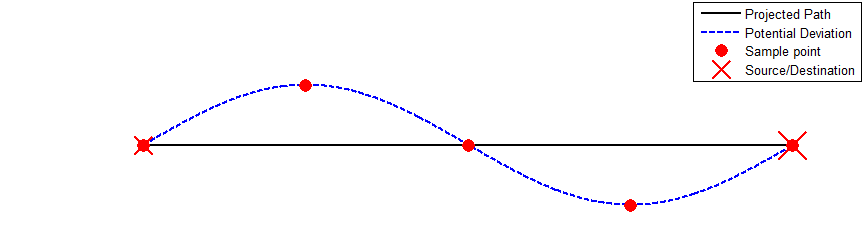
\includegraphics[scale = 0.75]{Pictures/2ndHarmonic.png}
	
	\caption{The second harmonic deviation from a straight line path, showing required sample points}
	\label{fig:2ndHarmonic}
\end{figure}
The regularity of the period was also of concern to the `sampling' ability of a given constellation. A more regular period represented a more `reliable' sampling rate and therefore a lower standard deviation of period was desired. As discussed in Section \ref{sec:periodicity_stats}, the distribution of periods which fitted a student's t distribution with an undefined standard deviation represented the greatest confidence for regularity. These cases were automatically assigned a full 10/10 score, whilst other situations with non-singular standard deviations were calculated using Equation \ref{eqn:linearisation_up} with the minimum set to `0'.

\subsection{Results}
The three highest scoring constellations, with their relative scores, are shown in Table \ref{tab:decMatRes}. The decision matrix heavily favoured the constellations with more satellites and lower altitudes. A higher number of satellites had a positive impact on the access-coverage characteristics, whilst lower altitude satellites had much more favourable potential signal strengths. A different set of results could be produced if the decision matrix were weighted according to a different set of design principles. The distribution of scores showed that most scores fell within a tight band around 70 \%, as seen in Figure \ref{fig:decisionMatrixHist}

% Table generated by Excel2LaTeX from sheet 'Sheet1'
\begin{table}[htbp]
  \centering
  \caption{The three highest scoring constellations after applying the weighted decision matrix}
    \begin{tabular}{rlrr}
    \toprule
    Case Number & Satellite Parameters &       & Score (\%) \\
    \midrule
    \multicolumn{1}{c}{\multirow{1}[10]{*}{22}} & Altitude (km above mean radius of Earth) & 700   & \multicolumn{1}{c}{\multirow{1}[10]{*}{78.45}} \\
    \multicolumn{1}{c}{} & Inclination (deg) & 60    & \multicolumn{1}{c}{} \\
    \multicolumn{1}{c}{} & Number of Planes & 3     & \multicolumn{1}{c}{} \\
    \multicolumn{1}{c}{} & Number of Satellites per plane & 6     & \multicolumn{1}{c}{} \\
    \multicolumn{1}{c}{} & Number of Satellites (Total) & 18    & \multicolumn{1}{c}{} \\ \hline
    \multicolumn{1}{c}{\multirow{1}[10]{*}{21}} & Altitude (km above mean radius of Earth) & 700   & \multicolumn{1}{c}{\multirow{1}[10]{*}{74.39}} \\
    \multicolumn{1}{c}{} & Inclination (deg) & 60    & \multicolumn{1}{c}{} \\
    \multicolumn{1}{c}{} & Number of Planes & 3     & \multicolumn{1}{c}{} \\
    \multicolumn{1}{c}{} & Number of Satellites per plane & 5     & \multicolumn{1}{c}{} \\
    \multicolumn{1}{c}{} & Number of Satellites (Total) & 15    & \multicolumn{1}{c}{} \\ \hline
    \multicolumn{1}{c}{\multirow{1}[10]{*}{1}} & Altitude (km above mean radius of Earth) & 400   & \multicolumn{1}{c}{\multirow{1}[10]{*}{73.22}} \\
    \multicolumn{1}{c}{} & Inclination (deg) & 60    & \multicolumn{1}{c}{} \\
    \multicolumn{1}{c}{} & Number of Planes & 3     & \multicolumn{1}{c}{} \\
    \multicolumn{1}{c}{} & Number of Satellites per plane & 4     & \multicolumn{1}{c}{} \\
    \multicolumn{1}{c}{} & Number of Satellites (Total) & 12    & \multicolumn{1}{c}{} \\
    \bottomrule
    \end{tabular}%
  \label{tab:decMatRes}%
\end{table}%

\begin{figure}[H]
	\centering
	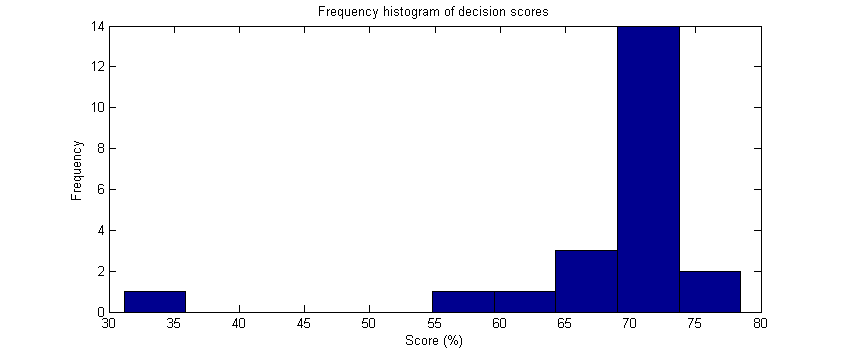
\includegraphics[scale = 0.6]{Pictures/decisionMatrixHist.png}
	
	\caption{Distribution of scores from decision matrix}
	\label{fig:decisionMatrixHist}
\end{figure}


\section{Special Case Study - MH370}\label{sec:mh370}
The Malaysia Airlines Flight MH370 disappeared on the evening of March the 7th, GMT after losing contact with air traffic control at approximately 5:20pm GMT \cite{Rahman2014}. Publicly available data of the flight after 5:21pm GMT was unavailable, at which point the flight was approximately 6.92$^\circ$N and 101.70$^\circ$E \cite{FlightRadar}. Military radar information suggests that the flight visited a series of known way points west of the planned flight path before being completely lost \cite{ReutersRadar}. Data from satellite pings and international search efforts suggested that the aircraft may have crashed in the Indian Ocean, as illustrated in Figure \ref{fig:mh370_probability_map} \cite{PaulColg, Pandey, ABCNews2014}. As of April 16th 2014, there is an ongoing international effort to attempt to locate the possible crash site and location of the debris from the MH370. 
\begin{figure}[H]
	\centering
	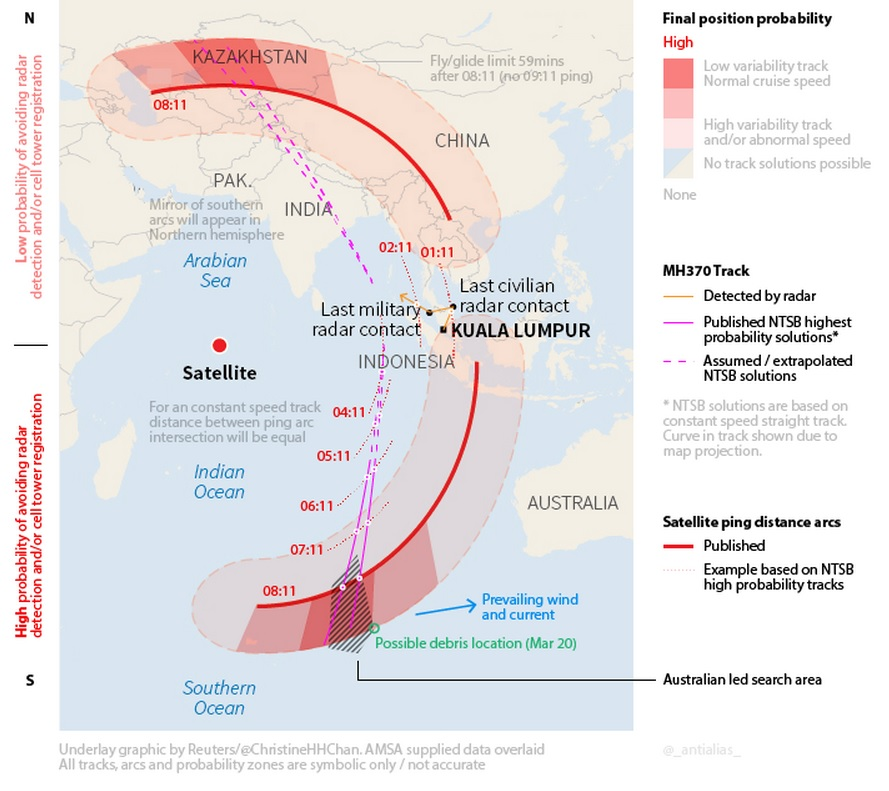
\includegraphics[scale = 0.5]{Pictures/mh370_probability_map.jpg}
	
	\caption[Probability map of possible crash locations of the MH370]{Probability map of possible crash locations of the MH370, reproduced from \cite{PaulColg}}
	\label{fig:mh370_probability_map}
\end{figure}
\subsection{Simulation}
As seen in Figure \ref{fig:mh370_probability_map}, it is most likely that the majority of the flight time after lost radar coverage would be spent over oceanic regions where an ADS-B constellation could provide coverage. The best performing constellation (18 satellites at 700km altitude) was tested against an estimated flight path for the MH370 alongside its standard path. This estimated path assumed that the flight terminated over the Indian Ocean, as shown in Figure \ref{fig:mh370_tot}. For the sake of coverage analysis it was assumed that the ADS-B transponder remained operational for the duration of the flight.
\begin{figure}[H]
	\centering
	\includegraphics[scale = 0.45]{Pictures/mh370_tot.png}
	
	\caption{Simulated MH370 flight path with 18 satellite constellation}
	\label{fig:mh370_tot}
\end{figure}
\subsection{Results}
The coverage results are summarised in Table \ref{tab:mh370_results}. Results showed that the 18 satellite constellation would have allowed for near constant coverage, with the flight only being out of sight for 10\% of the flight. The high number of discrete accesses for the one flight would have also allowed for deviations in the flight path to be detected early and accurately mapped with many sample points.
\begin{table}[htbp]
  \centering
  \caption{Results from MH370 simulation using 18 satellites}
    \begin{tabular}{lr}
    \toprule
    Parameter & Value \\
    \midrule
    Coverage Gap Fraction & 0.10\% \\
    Discrete Accesses & 20.00 \\
    Maximum Gap & 309.72 seconds \\
    Minimum RX Power & -139.95 dBW \\
    \bottomrule
    \end{tabular}%
  \label{tab:mh370_results}%
\end{table}%
\subsection{Discussion}
The results from this simulation show that the 18 satellite constellation would have provided coverage to almost continually track the MH370 during its flight. If the ADS-B transponder remained operational during the flight, the probable crash and debris locations could be much smaller providing for a much more feasible search area.

The exact status of the ADS-B transponder during the flight is currently unknown. No ADS-B data exists beyond of that reported by \cite{FlightRadar}. ADS-B receivers in the vicinity of this disappearance suggest that the ADS-B transponder was inoperable after this period. In this case the constellation would have not been able to track the entirety of the deviated flight path. However, the high effective ADS-B sample rate of the 18 satellite constellation would have provided a more accurate estimation as to the exact time and location when the ADS-B signal would have been lost. This could have aided in search efforts and generated potential flight paths with greater confidence.

\chapter{Conclusions and Future Work}\label{part:concl}
With further development and refinement of small satellite based ADS-B technology, near constant global coverage can be achieved with a constellation of CubeSats in LEO. The experiments conducted showed that all chosen constellations provide the geographic coverage for the major transoceanic flight corridors. Varying degrees of coverage time and update rate effectiveness was achieved by varying constellation parameters, with the best result achieved by an 18 satellite constellation at an altitude of 700km. Future work needs to be conducted in order to create more realistic models for full system analysis and further design.
\section{Conclusions}
The suite of simulations showed that constellations with higher altitude or a higher number of satellites provided more raw coverage time. A higher altitude allowed for a greater sensor footprint, meaning that a trans-oceanic flight would stay in-view for longer. Having more satellites increased the probability of a satellite being above a trans-oceanic flight at any one point in time. The effect of this was significant enough such that the penalty of the increased constellation cost was offset by the net benefit to the coverage opportunities.

Despite the improved geographic coverage performance of high altitude constellations, low altitude constellations showed a marked improvement in signal performance. Less distance was required to travel by any one ADS-B transmission at lower altitudes, resulting in lower signal loss. This effect was dramatic enough such that the lowest altitude constellation performed better than most other constellations as seen in Table \ref{tab:decMatRes}.

The inclination trend analysis suggested that a constellation with all satellites inclined at 90 degrees may represent the best coverage trade-off between the three flights. This inclination represented the best possible geometric configuration for full global coverage. However, the nature of one-dimensional parameter variance in the tests conducted and the weighted decision matrix meant that the 90 degree inclination configuration did not feature in the `best choices', with system coverage overriding the potential cost of the system as a performance metric. 
\subsection{Chosen Constellation}
The results from the weighted decision matrix show that a satellite constellation with parameters as defined in Table \ref{tab:18sat_winner} is the best performing space based ADS-B system of those tested. This particular constellation performed strongly in being able to provide a high level of coverage for the three trans-oceanic flights studied in this thesis. A 3D model of this constellation is shown in Figure \ref{fig:18sat_3D} and the ground tracks in Figure \ref{fig:18sat_groundtrack}

% Table generated by Excel2LaTeX from sheet 'Sheet2'
\begin{table}[htbp]
  \centering
  \caption{18 satellite configuration with the best score}
    \begin{tabular}{lr}
    \toprule
    Parameter & Value \\
    \midrule
    Altitude (km above mean radius of Earth) & 700 \\
    Inclination (deg) & 60 \\
    Number of Planes & 3 \\
    Plane Separation (deg RAAN) & 120 \\
    Number of Satellites per plane & 6 \\
    True Anomaly Separation (deg) & 60 \\
    Number of Satellites (Total) & 18 \\
    \bottomrule
    \end{tabular}%
  \label{tab:18sat_winner}%
\end{table}%

\begin{figure}[htbp]
	\centering
	\includegraphics[scale = 0.4]{Pictures/18sat_3D.png}
	
	\caption{18 satellite configuration rendered in STK showing a) the view above North America and b) the view above the Arctic}
	\label{fig:18sat_3D}
\end{figure}

\begin{figure}[htbp]
	\centering
	\includegraphics[scale = 0.6]{Pictures/18sat_groundtrack.png}
	
	\caption{Ground track of the 18 satellite configuration, rendered in STK}
	\label{fig:18sat_groundtrack}
\end{figure}

This particular result shows that a higher-number of satellites performs more favourably when considering ADS-B coverage requirements. Interestingly, a fewer satellites in a lower orbit performed almost as well due to dramatically increased communication link quality. In this case, the benefit of having more effective coverage outweighed the benefit of having less satellites. This may not be the case if the decision matrix was weighted more heavily to budgetary considerations.  The tests conducted only examined variation of one parameter at a time and can not provide a conclusion on whether a combination of two or more parameters would result in better performance.

\section{Future Work}
The following work should be conducted in order to fully develop a set of mission and system specifications for a CubeSat based ADS-B system.
\subsection{Full Parametric Study}
The findings of this thesis are as a result of one-dimensional parameter studies. As such they are indicative of general trends observed when varying only one constellation parameter at a time. This only gives an indication of what the best possible satellite configuration could be. In order to determine the global best performer, a full n-dimensional parametric study should be carried out, simulating all possible variations of all the orbital parameters.  In particular, given the results of the weighted decision matrix in Section \ref{sec:decision_matrix}, it is expected that a lower altitude (approximately 400km) with a higher number of satellites could produce a more optimal result than any constellation tested in this thesis. The simulations created for this thesis form a good basis from which a full parametric set of simulations can be generated.

\subsection{Transmitter Receiver Model Improvements}
As noted in Section \ref{sec:perfMetrics}, the simple transmitter and receiver models used produced an unrealistic link-budget characterisation for ADS-B communication links. Although received isotropic power is a good metric to compare constellation performance, the link budget results in this thesis do not represent realistic system behaviour. Incorporating a more sophisticated antenna design and better radio-frequency front-end into the communication models would more accurately characterise ADS-B signal performance. This would be necessary in further systems analysis and design.

\subsection{Ground Link}
Further study needs to be performed into how to establish a regular downlink between the satellites in the constellation and a ground station. The regularity of this downlink would determine the `total system update rate' or the speed with which data on all detected flights can be disseminated to ANSPs and therefore general use. Potential methods could be to
\begin{itemize}
	\item Use network of community-run amateur radio ground stations
	\item Transmit downlink packets to currently in-orbit communication constellations, such as Iridium or Globalstar
	\item Relay raw ADS-B data to airports and terrestrial ADS-B receivers.
\end{itemize}
The benefits and potential performance of each option needs to be further explored before a full space-based ADS-B solution can be designed.


%\section{Link Budget Analysis}
\begin{itemize}
	\item Path Loss
\end{itemize}

\subsection{Potential model}
\textbf{Proba V} \cite{TheEuropeanSpaceAgency2013}\\
Instrument: The ADS-B device is provided by DLR and SES Techcom of Luxembourg, the main objective is to test (space qualify) the ADS-B electronic boards in flight-representative configuration to evaluate TID (Total Ionizing Dose). The basic design concept of the ADS-B receiver (1090ES RX) is a single conversion superheterodyne receiver with a down conversion of 1090 MHz to an intermediate frequency of 70 MHz. The IF sampling at 70 MHz is done by a 16 bit ADC at 105 Msps (Mega samples per second). The digital part of the receiver is built around a Cyclone IV FPGA from Altera which combines the complete data processing as well as the communication with the onboard computer of the PROBA-V spacecraft. The digital and the RF section of the receiver are built on an individual PCB each, connected with a 37 pin MDM PCB connector. 60) \

\subsection{Ground}
Survey of Mode S transponders show
\begin{itemize}
	\item AXP340 - 240W
	\item GTX330 - 250W, (-740dBm rx sensitivity for 90 percent)
	\item 125watt minimum \cite{ADSB_DOT}.
\end{itemize}

\subsection{Mode S}
\begin{itemize}
	\item Pulse position modulation (pulse offset = 0 (missed edge))
	\item 
\end{itemize}
\subsection{Orbit Parameters}
\subsubsection{J2 Effect Formula}
\begin{align}
	\dot{\Omega} = \dfrac{-9.9597408}{(1-e^2)^2} \left(\dfrac{R}{a}\right)^{3.5} \cos i
\end{align}
Solve for $\dot{\Omega} = 0$ to find sun synchronus orbit inclination.

\newpage
\addcontentsline{toc}{chapter}{References}
\bibliographystyle{IEEEtran}
\bibliography{references}

\newpage
\addcontentsline{toc}{part}{Appendices}
\appendix

\chapter{2013 AIAA Region VII-AU Student Conference \\ Full Text of Accepted Paper}
\label{app:aiiastuconf}
\includepdf[pages={1-10}]{papers/tnguyen_aiaaStudentConference2013v4.pdf}
\chapter{65th International Astronautical Congress \\ Abstract and Acceptance Letter}
\label{app:iac_2014}
\includepdf[pages={1}]{papers/tnguyen_IAC2014_absract.pdf}
\includepdf[pages={1-2}]{papers/tnguyen_IAC2014_letter.pdf}

\section{Experimental Parameters}
\label{app:all_parameters}
% Table generated by Excel2LaTeX from sheet 'Sheet1'
\begin{table}[htbp]
	\tiny
  \centering
  \caption{Orbital parameters of all experimental cases studied}
    \begin{tabular}{p{1cm}lp{1cm}p{12mm}p{10mm}p{10mm}p{1cm}lp{1cm}p{1cm}}
    \toprule
    Case Number & Section & Altitude (km) & Semi-major axis (km) & Inclination (deg) & Satellites (Total) &Satellites per plane & Planes & Plane separation (deg RAAN) & True Anomaly Separation \\
    \midrule
    1     &       & 400   & 6778.14 & 60    & 12    & 4     & 3     & 120   & 90 \\
    2     &       & 450   & 6828.14 & 60    & 12    & 4     & 3     & 120   & 90 \\
    3     &       & 500   & 6878.14 & 60    & 12    & 4     & 3     & 120   & 90 \\
    4     &       & 550   & 6928.14 & 60    & 12    & 4     & 3     & 120   & 90 \\
    5     &       & 600   & 6978.14 & 60    & 12    & 4     & 3     & 120   & 90 \\
    6     &       & 650   & 7028.14 & 60    & 12    & 4     & 3     & 120   & 90 \\
    7     &       & 700   & 7078.14 & 60    & 12    & 4     & 3     & 120   & 90 \\
    8     &       & 750   & 7128.14 & 60    & 12    & 4     & 3     & 120   & 90 \\
    9     &       & 800   & 7178.14 & 60    & 12    & 4     & 3     & 120   & 90 \\
    10    &       & 700   & 7078.14 & 30    & 12    & 4     & 3     & 120   & 90 \\
    11    &       & 700   & 7078.14 & 40    & 12    & 4     & 3     & 120   & 90 \\
    12    &       & 700   & 7078.14 & 50    & 12    & 4     & 3     & 120   & 90 \\
    13    &       & 700   & 7078.14 & 60    & 12    & 4     & 3     & 120   & 90 \\
    14    &       & 700   & 7078.14 & 70    & 12    & 4     & 3     & 120   & 90 \\
    15    &       & 700   & 7078.14 & 80    & 12    & 4     & 3     & 120   & 90 \\
    16    &       & 700   & 7078.14 & 90    & 12    & 4     & 3     & 120   & 90 \\
    17    &       & 700   & 7078.14 & 60    & 3     & 1     & 3     & 120   & 360 \\
    18    &       & 700   & 7078.14 & 60    & 6     & 2     & 3     & 120   & 180 \\
    19    &       & 700   & 7078.14 & 60    & 9     & 3     & 3     & 120   & 120 \\
    20    &       & 700   & 7078.14 & 60    & 12    & 4     & 3     & 120   & 90 \\
    21    &       & 700   & 7078.14 & 60    & 15    & 5     & 3     & 120   & 72 \\
    22    &       & 700   & 7078.14 & 60    & 18    & 6     & 3     & 120   & 60 \\
    \bottomrule
    \end{tabular}%
  \label{tab:allExperiments}%
\end{table}%

\chapter{Statistical Models} \label{sec:stats}
\section{Student's t-Location Scale Distribution}
The majority of data analysed statistically in this thesis found that a Students t distribution with a location-scale transformation provided the best fit statistical model. The periodicity analysis of satellite-revisit time showed slight bimodal behaviour, resulting in heavy tails, typical of a `t Location-Scale Distribution' (CITE). 

The Student's t distribution probability density function (PDF) is given by
\begin{align}
	f_X(x) = \dfrac{\Gamma\left(\frac{\nu+ 1}{2}\right)}{\sqrt{v\pi} \Gamma \left(\frac{\nu}{2}\right)} \left( 1 + \dfrac{x^2}{\nu} \right) ^{-\frac{\nu + 1}{2}} \label{eqn:students_t}
\end{align}
where $\nu$ is the parameter defined as the `degrees of freedom' and $\Gamma$ is the standard gamma function. To shift and scale the data, we need to apply the location scale transformation to the random variable $X$
\begin{align}
	Y = \sigma X + \mu \label{eqn:locscale_transform}
\end{align}
the probability density function then becomes 
\begin{align}
	f_Y(y) = \dfrac{\Gamma\left(\frac{\nu+ 1}{2}\right)}{\sigma\sqrt{v\pi} \Gamma \left(\frac{\nu}{2}\right)} \left( 1 + \dfrac{1}{\nu} \left(\dfrac{x - \mu }{\sigma}\right)^2 \right) ^{-\frac{\nu + 1}{2}} \label{eqn:t_locscale}
\end{align}
In Section \ref{sec:prob_distro}, Equation (\ref{eqn:t_locscale}) is shown to be distribution of best fit for most sets of data of interest. The errors observed between the fitted distribution and the observed frequencies were within acceptable ranges for the purposes described later in Section \ref{sec:prob_distro}.

The parameters analysed in Section \ref{sec:prob_distro} required a measure of the variance of the data. For the Student's t distribution described by Equation (\ref{eqn:students_t}), this is given by
\begin{align}
	\text{Variance} = \dfrac{\nu}{\nu-2}.
\end{align}
With the location-scale transformation (\ref{eqn:locscale_transform}), the variance is described in terms of the three parameters $\nu, \mu$ and $\sigma$ by
\begin{align}
	\text{Variance} = \dfrac{\nu}{\nu-2}.
\end{align}

CALCULATE VARIANCE MANUALLY?


%\section{CubeSat Drawings} \label{app:cubesat}



\end{document}